\FloatBarrier

\section{Conclusion}

The SOM-VAE can recover topologically interpretable state representations on time series and static data.
It provides an improvement to standard methods in terms of clustering performance and offers a way to learn discrete two-dimensional representations of the data manifold in concurrence with the reconstruction task.
It introduces a new way of overcoming the non-differentiability of the discrete representation assignment and contains a gradient-based variant of the traditional self-organizing map that is more performant than the original one.
%The probabilistic component of our model can be learned end-to-end and concurrently with the rest of the architecture, while offering predictive performance close to the maximum likelihood solution and further improving the clustering on noisy data.
On a challenging real world medical data set, our model learns more informative representations with respect to medically relevant prediction targets than competitor methods.
%The probabilistic model component improves the clustering in this setting.
The learned representations can be visualized in an interpretable way and could be helpful for clinicians to understand patients' health states and trajectories more intuitively.

It will be interesting to see in future work whether the probabilistic component can be extended to not just improve the clustering and interpretability of the whole model, but also enable us to make predictions.
Promising avenues in that direction could be to increase the complexity by applying a higher order Markov Model, a Hidden Markov Model or a Gaussian Process.
Another fruitful avenue of research could be to find more theoretically principled ways to overcome the non-differentiability and compare them with the empirically motivated ones.
Lastly, one could explore deviating from the original SOM idea of fixing a latent space structure, such as a 2D grid, and learn the neighborhood structure as a graph directly from data.


\subsection*{Acknowledgments}

FL is supported by the Max Planck/ETH Center for Learning Systems.
MH is supported by the Grant No. 205321\_176005 ``Novel Machine Learning Approaches for Data from the Intensive Care
Unit'' of the Swiss National Science Foundation (to GR).
VF, FL, MH and HS are partially supported by ETH core funding (to GR).
We thank Natalia Marciniak for her administrative efforts; Marc Zimmermann for technical support; Gideon Dresdner, Stephanie Hyland, Viktor Gal, Maja Rudolph and Claire Vernade for helpful discussions; and Ron Swanson for his inspirational attitude.
\beginsupplement

\newpage

\appendix

\section*{Appendix}

\section{Self-organizing maps}\label{sec:SOMs}

The general idea of a self-organizing map (SOM) is to approximate a data manifold in a high-dimensional continuous space with a lower dimensional discrete one \citep{Kohonen1998}.
It can therefore be seen as a nonlinear discrete dimensionality reduction.
The mapping is achieved by a procedure in which this discrete representation (the \emph{map}) is randomly embedded into the data space and then iteratively optimized to approach the data manifold more closely.

The map consists of $k$ nodes $V=\{v_1, \dots , v_k\}$, where every node corresponds to an embedding in the data space $e_v \in \mathbb{R}^d$ and a representation in the lower-dimensional discrete space $m_v \in M$, where usually $M \subset \mathbb{N}^2$.
There are two different geometrical measures that have to be considered during training: the neighborhood function $N(m_u, m_{\tilde{v}})$ that is defined on the low-dimensional map space and the Euclidean distance $D (e_u, e_{\tilde{v}}) = \| e_u - e_{\tilde{v}} \|_2$ in the high-dimensional data space.
The SOM optimization tries to induce a coupling between these two properties, such that the topological structure of the representation reflects the geometrical structure of the data.


\begin{algorithm}
\caption{Self-organizing map training}
\label{alg:som_train}

\begin{algorithmic}
	\Require data set $\mathcal{D} = \{x_1, \dots ,x_n \; \vert \; x_i \in \mathbb{R}^d\}$, number of nodes $k$, neighborhood function $N(\cdot)$, step size $\eta$
	\State initialize set of $k$ nodes $V=\{v_1, \dots , v_k\}$
	\State initialize embeddings $e_v \in \mathbb{R}^d \; \forall \; v \in V$
	\While{not converged}
	\ForAll {$x_i \in \mathcal{D}$}
		\State find the closest SOM node $\tilde{v} := \argmin_{v \in V} \| x_i - e_v \|_2$
		\State update node embedding $e_{\tilde{v}} \gets e_{\tilde{v}} + \eta \, (x_i - e_{\tilde{v}})$
		\ForAll {$u \in V \backslash \tilde{v}$}
			\State update neighbor embedding $e_u \gets e_u + \eta \, N(m_{\tilde{v}}, m_u) (x_i - e_u)$
		\EndFor
	\EndFor
	\EndWhile
\end{algorithmic}
	
\end{algorithm}

The SOM training procedure is described in Algorithm~\ref{alg:som_train}.
During training on a data set $\mathcal{D}$, a winner node $\tilde{v}$ is chosen for every point $x_i$ according to the Euclidean distance of the point and the node's embedding in the data space.
The embedding vector for the winner node is then updated by pulling it into the direction of the data point with some step size $\eta$.
The embedding vectors of the other nodes are also updated -- potentially with a smaller step size -- depending on whether they are neighbors of the winner node in the map space $M$.

The neighborhood is defined by the neighborhood function $N(m_u, m_{\tilde{v}})$.
There can be different design choices for the neighborhood function, e.g.\ rectangular grids, hexagonal grids or Gaussian neighborhoods.
For simplicity and ease of visualization, we usually choose a two-dimensional rectangular grid neighborhood in this paper.

In this original formulation of the SOM training, the nodes are updated one by one with a fixed step size.
In our model, however, we use a gradient-based optimization of their distances to the data points and update them in minibatches.
This leads to larger step sizes when they are farther away from the data and smaller step sizes when they are close.
Overall, our gradient-based SOM training seems to perform better than the original formulation (see Tab.~\ref{tab:performance}).

It also becomes evident from this procedure that it will be very hard for the map to fit disjoint manifolds in the data space.
Since the nodes of the SOM form a fully connected graph, they do not possess the ability to model spatial gaps in the data.
We overcome this problem in our work by mapping the data manifold with a variational autoencoder into a lower-dimensional latent space.
The VAE can then learn to close the aforementioned gaps and map the data onto a compact latent manifold, which can be more easily modeled with the SOM.



\section{Implementation details}\label{sec:implementation}

The hyperparameters of our model were optimized using Robust Bayesian Optimization with the packages \texttt{sacred} and \texttt{labwatch} \citep{Greff2017a} for the parameter handling and \texttt{RoBo} \citep{Klein2017} for the optimization, using the mean squared reconstruction error as the optimization criterion.
Especially the weighting hyperparameters $\alpha, \beta, \gamma$ and $\tau$ (see Eq.~\eqref{eq:L_somvae} and Eq.~\eqref{eq:L_prob}) have to be tuned carefully, such that the different parts of the model converge at roughly the same rate.
We found that 2000 steps of Bayesian optimization sufficed to yield a performant hyperparameter assignment.

Since our model defines a general framework, some competitor models can be seen as special cases of our model, where certain parts of the loss function are set to zero or parts of the architecture are omitted.
We used the same hyperparameters for those models.
For external competitor methods, we used the hyperparameters from the respective publications where applicable and otherwise the default parameters from their packages.
The models were implemented in TensorFlow \citep{GoogleResearch2015} and optimized using Adam \citep{Kingma2015}.


\section{Clustering performance measures}\label{sec:clustering_performance}

Given that one of our most interesting tasks at hand is the clustering of data, we need some performance measures to objectively compare the quality of this clustering with other methods.
The measures that we decided to use and that have been used extensively in the literature are \emph{purity} and \emph{normalized mutual information} (NMI) \citep{Manning2008}.
We briefly review them in the following.

Let the set of ground truth classes in the data be $C = \{ c_1, c_2, \dots, c_J \}$ and the set of clusters that result from the algorithm $\Omega = \{ \omega_1, \omega_2, \dots, \omega_K \}$.
The \emph{purity} $\pi$ is then defined as $\pi(C, \Omega) = \frac{1}{N} \sum_{k = 1}^K \max_j \vert \omega_k \cap c_j \vert$ where $N$ is the total number of data points.
Intuitively, the purity is the accuracy of the classifier that assigns the most prominent class label in each cluster to all of its respective data points.

While the purity has a very simple interpretation, it also has some shortcomings.
One can for instance easily observe that a clustering with $K = N$, i.e.\ one cluster for every single data point, will yield a purity of $1.0$ but still probably not be very informative for most tasks.
It would therefore be more sensible to have another measure that penalizes the number of clusters.
The normalized mutual information is one such measure.

The NMI is defined as $\textit{NMI}(C, \Omega) = \frac{2 \; I(C, \Omega)}{H(C) + H(\Omega)}$ where $I(C, \Omega)$ is the mutual information between $C$ and $\Omega$ and $H(\cdot)$ is the Shannon information entropy.
While the entropy of the classes is a data-dependent constant, the entropy of the clustering increases with the number of clusters.
It can therefore be seen as a penalty term to regularize the trade-off between low intra-cluster variance and a small number of clusters.
Both NMI and purity are normalized, i.e.\ take values in $[0,1]$.



\section{Experimental details}


\subsection{Clustering on MNIST and Fashion-MNIST} \label{sec:mnist_appendix}

Additionally to the results in Table~\ref{tab:performance}, we performed experiments to assess the influence of the number of clusters $k$ on the clustering performance of our method.
We chose different values for $k$ between 4 and 64 and tested the clustering performance on MNIST and Fashion-MNIST (Tab.~\ref{tab:k_performance}).

\begin{table}
    \centering
    \caption{Performance comparison of our method with different numbers of clusters in terms of purity and normalized mutual information on different benchmark data sets. The values are the means of 10 runs and the respective standard errors.}
    \begin{tabular}{lrrrr}
        \toprule
         & \multicolumn{2}{c}{MNIST} & \multicolumn{2}{c}{Fashion-MNIST} \\
        \cmidrule(rl){2-3}
        \cmidrule(rl){4-5}
        Number of clusters & \multicolumn{1}{c}{Purity} & \multicolumn{1}{c}{NMI} & \multicolumn{1}{c}{Purity} & \multicolumn{1}{c}{NMI} \\
         \midrule
         $k = 4$ & 0.364 $\pm$ 0.009 & 0.378 $\pm$ 0.018 & 0.359 $\pm$ 0.005 & 0.431 $\pm$ 0.008\\
         $k = 9$ & 0.626 $\pm$ 0.006 & 0.554 $\pm$ 0.004 & 0.558 $\pm$ 0.007 & 0.560 $\pm$ 0.006\\
         $k = 16$ & 0.721 $\pm$ 0.006 & 0.587 $\pm$ 0.003 & 0.684 $\pm$ 0.003 & \textbf{0.589 $\pm$ 0.003}\\
         $k = 25$ & 0.803 $\pm$ 0.003 & \textbf{0.613 $\pm$ 0.002} & 0.710 $\pm$ 0.003 & 0.572 $\pm$ 0.002\\
         $k = 36$ & 0.850 $\pm$ 0.002 & \textbf{0.612 $\pm$ 0.001} & 0.732 $\pm$ 0.002 & 0.556 $\pm$ 0.002\\
         $k = 49$ & 0.875 $\pm$ 0.002 & 0.608 $\pm$ 0.001 & 0.750 $\pm$ 0.002 & 0.545 $\pm$ 0.001\\
         $k = 64$ & \textbf{0.894 $\pm$ 0.002} & 0.599 $\pm$ 0.001 & \textbf{0.758 $\pm$ 0.002} & 0.532 $\pm$ 0.001\\
         \bottomrule
    \end{tabular}
    \label{tab:k_performance}
\end{table}

It can be seen that the purity increases monotonically with $k$, since it does not penalize larger numbers of clusters (see Sec.~\ref{sec:clustering_performance}).
The NMI, however, includes an automatic penalty for misspecifying the model with too many clusters.
It therefore increases first, but then decreases again for too large values of $k$.
The optimal $k$ according to the NMI seems to lie between 16 and 36.


\subsection{Interpretable representations of chaotic time series}\label{sec:lorenz_appendix}

The Lorenz system is the system of coupled ordinary differential equations defined by
%
\begin{equation*}
	\frac{dX}{dt} = a (Y - X) \hskip 4em
	\frac{dY}{dt} = X (b - Z) - Y \hskip 4em
	\frac{dZ}{dt} = XY - cZ
\end{equation*}
%
with tuning parameters $a$, $b$ and $c$. For parameter choices $a = 10$, $b = 28$ and $c = \frac{8}{3}$, the system shows chaotic behavior by forming a strange attractor \citep{Tucker1999} with the two attractor points being given by $p_{1,2} = \lbrack \pm \sqrt{c (b-1)}, \pm \sqrt{c (b-1)}, b-1 \rbrack^T$.

We simulated 100 trajectories of 10,000 time steps each from the chaotic system and trained the SOM-VAE as well as k-means on it with 64 clusters/embeddings respectively.
The system chaotically switches back and forth between the two attractor basins.
By computing the Euclidian distance between the current system state and each of the attractor points $p_{1,2}$, we can identify the current attractor basin at each time point.

In order to assess the interpretability of the learned representations, we have to define an objective measure of interpretability.
We define interpretability as the similarity between the representation and the system's ground truth macro-state.
Since representations at single time points are meaningless with respect to this measure, we compare the evolution of representations and system state over time in terms of their entropy.

We divided the simulated trajectories from our test set into spans of 100 time steps each.
For every subtrajectory, we computed the entropies of those subtrajectories in the real system space (macro-state and noise), the assigned attractor basin space (noise-free ground-truth macro-state), the SOM-VAE representation and the k-means representation.
We also observed for every subtrajectory whether or not a change between attractor basins has taken place.
Note that the attractor assignments and representations are discrete, while the real system space is continuous.
In order to make the entropies comparable, we discretize the system space into unit hypercubes for the entropy computation.
For a representation $\mathcal{R}$ with assignments $\mathcal{R}_t$ at time $t$ and starting time $t_{start}$ of the subtrajectory, the entropies are defined as
%
\begin{equation}
	H \left( \mathcal{R}, t_{start} \right) = H \left( \lbrace R_t \; \vert \; t_{start} \leq t < t_{start} + 100 \rbrace \right)
\end{equation}
%
with $H(\cdot)$ being the Shannon information entropy of a discrete set.


\subsection{Learning representations of acute physiological states in the ICU}\label{sec:ICU_appendix}

All experiments were performed on dynamic data extracted from the \texttt{eICU} Collaborative Research Database \citep{Goldberger2000}.
Irregularly sampled time series data were extracted from the raw tables and then resampled to a regular time grid using a combination of forward filling and missing value imputation using global population statistics.
We chose a grid interval of one hour to capture the rapid dynamics of patients in the ICU.

Each sample in the time-grid was then labeled using a dynamic variant of the \texttt{APACHE} score \citep{Knaus1985}, which is a proxy for the instantaneous physiological state of a patient in the ICU.
Specifically, the variables \texttt{MAP}, \texttt{Temperature}, \texttt{Respiratory rate}, \texttt{HCO3}, \texttt{Sodium}, \texttt{Potassium}, and \texttt{Creatinine} were selected from the score definition, because they could be easily defined for each sample in the \texttt{eICU} time series.
The value range of each variable was binned into ranges of normal and abnormal values, in line with the definition of the \texttt{APACHE} score, where a higher score for a variable is obtained for abnormally high or low values.
The scores were then summed up, and we define the predictive score as the \emph{worst (highest) score} in the next $t$ hours, for $t \in \{ 6, 12, 24 \}$.
Patients are thus stratified by their expected pathology in the near future, which corresponds closely to how a physician would perceive the state of a patient.
The training set consisted of 7000 unique patient stays, while the test set contained 3600 unique stays.


\subsection{Detailed analysis of \texttt{SOMVAEprob} patient states}
\label{subsec:detailed_icu}

As mentioned in the main text (see Fig \ref{fig:ICU_representations}) the \texttt{SOMVAEProb}
is able to uncover compact and interpretable structures in the latent space with respect
to future physiology scores. In this section we show results for acute physiology scores
in greater detail, analyze enrichment for future mortality risk, arguably the most
important severity indicator in the ICU, and explore phenotypes for particular 
physiological abnormalities.

% Acute physiology scores

\subsubsection*{Full results for future acute physiology scores}

\begin{figure}[h!]

\centering
\begin{subfigure}[t]{0.30\textwidth}
\centering
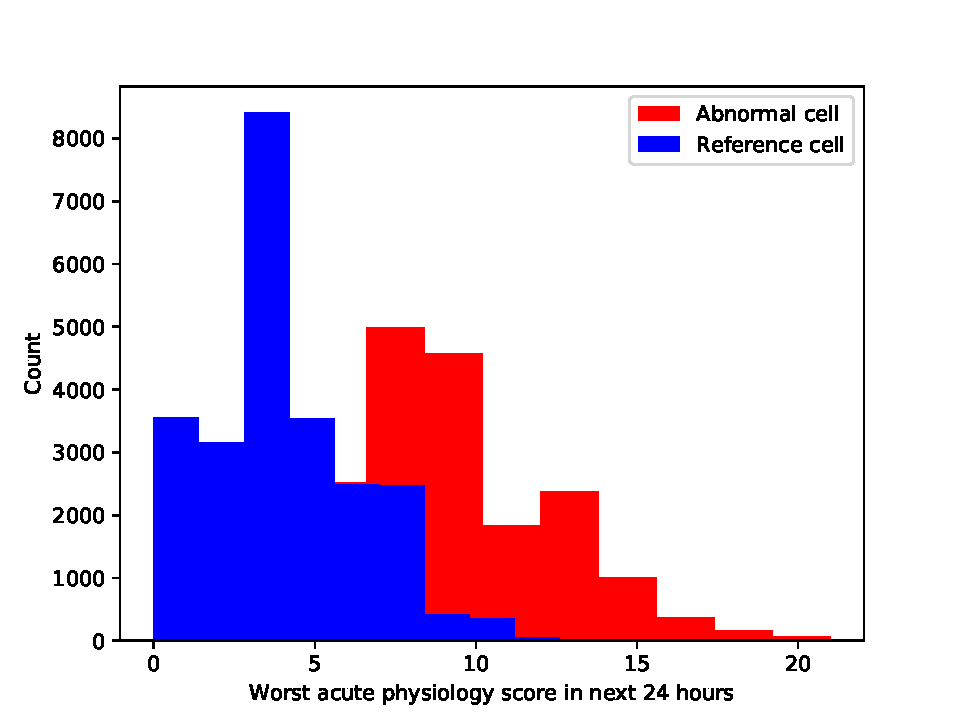
\includegraphics[scale=0.30]{./figures/icu_somvaeprob/distribution_cells}
\caption{Abnormal vs. reference cell}
\end{subfigure}
\begin{subfigure}[t]{0.30\textwidth}
\centering
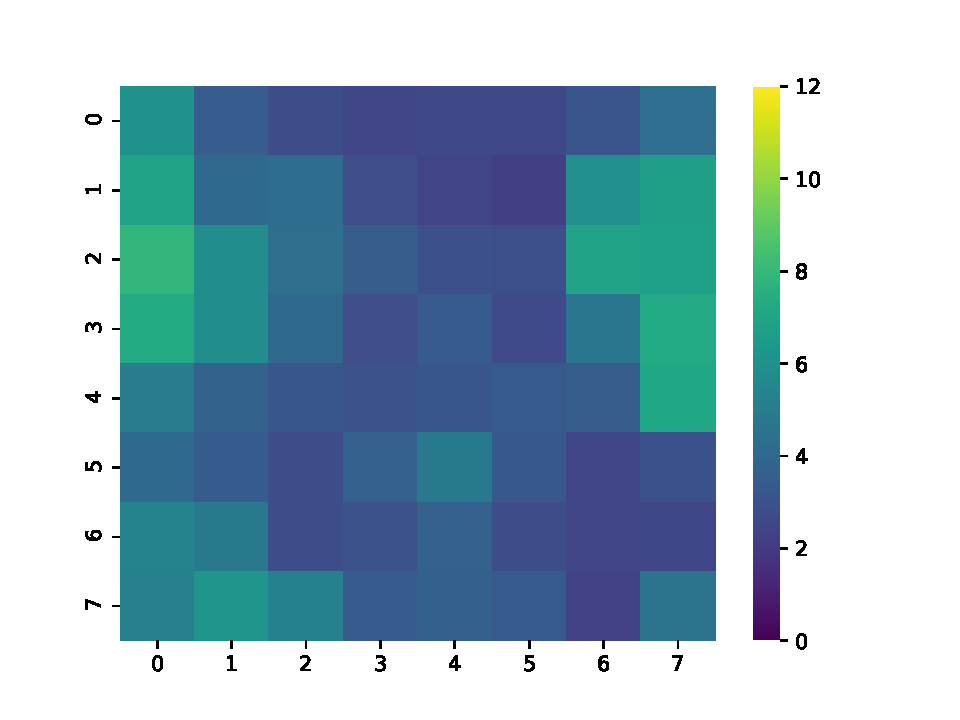
\includegraphics[scale=0.30]{./figures/icu_somvaeprob/detail_heatmaps_full_score_6}
\caption{Acute physiology score (6)}
\end{subfigure}
\begin{subfigure}[t]{0.30\textwidth}
\centering
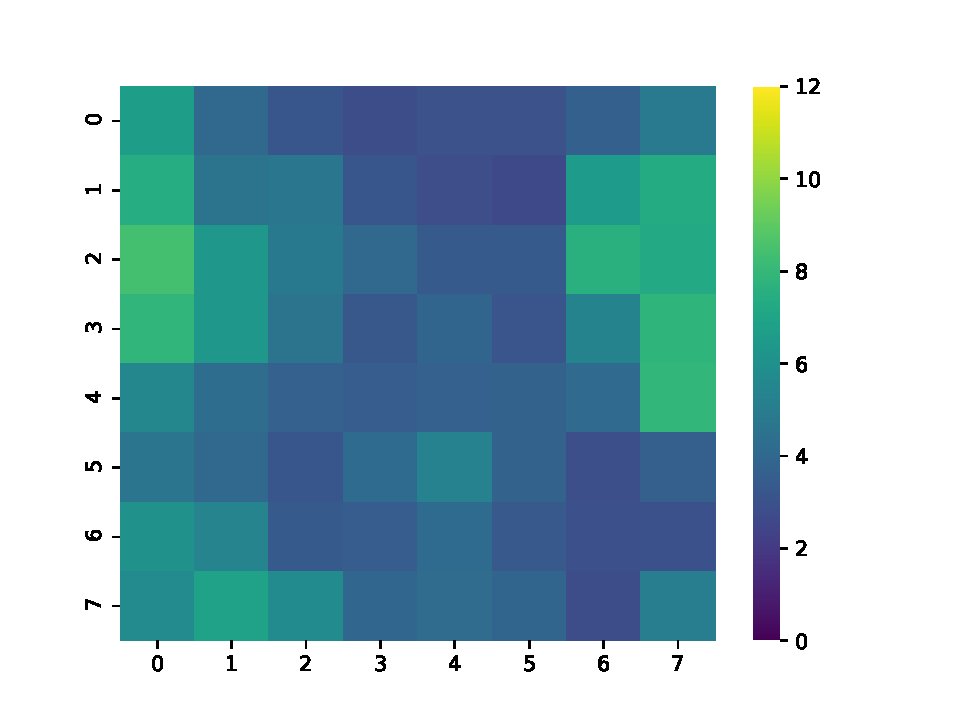
\includegraphics[scale=0.30]{./figures/icu_somvaeprob/detail_heatmaps_full_score_12}
\caption{ Acute physiology score (12)}
\end{subfigure}

\caption{(a) shows the difference in distribution of the acute
         physiology score in the next 24 hours, between time-points assigned to the most 
         abnormal cell in the \texttt{SOMVAEprob} map with coordinates [2,0] vs. 
         a normal cell chosen from the middle of the map with coordinates [4,3]. It is apparent that
         the distributions are largely disjoint, which means that the representation induced by 
         \texttt{SOMVAEprob} clearly distinguishes these risk profiles. Statistical tests for difference
         in distribution and location parameter are highly significant at p-values of $p \leq 10^{-3}$, as we
         have validated using a 2-sample $t$-test and Kolmogorov-Smirnov test. In (b-c) the enrichment 
         of the map for the mean acute physiology score in the next 6 and 12 hours is shown, for completeness.
         The enrichment patterns on the 3 maps, for the future horizons $\{6,12,24\}$, are almost identical, 
         which provides empirical evidence for the temporal stability of the \texttt{SOMVAEProb} embedding.}

\end{figure}

% Dynamic mortality in the next {12,24} hours

\subsubsection*{Dynamic mortality risk of patients on the \texttt{SOMVAEprob} map}

\begin{figure}[h!]
\centering
\begin{subfigure}[t]{0.47\textwidth}
\centering
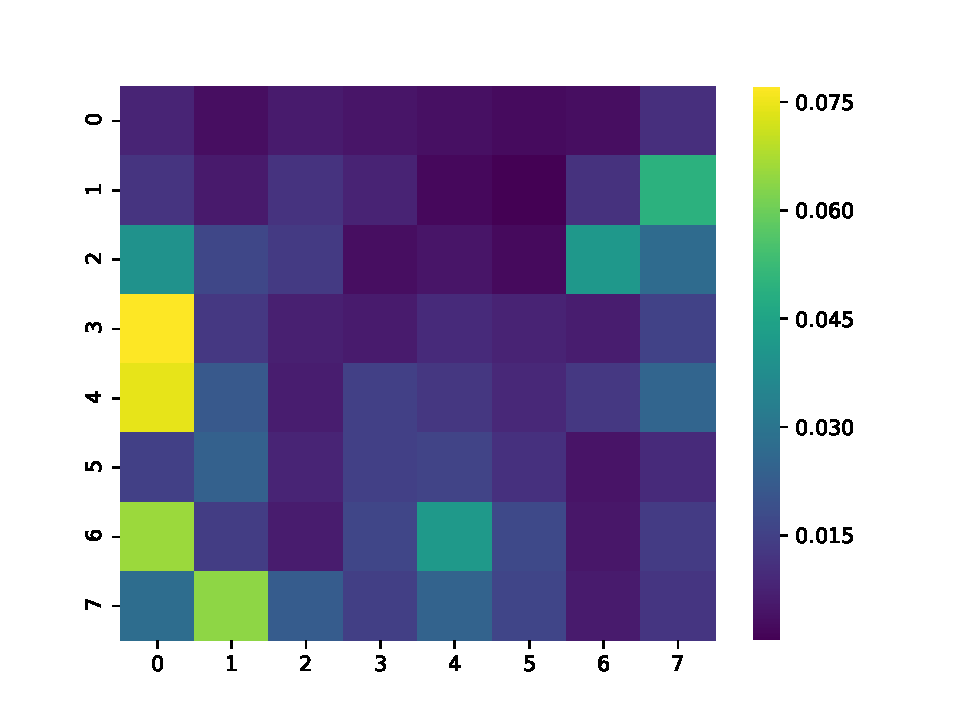
\includegraphics[scale=0.4]{./figures/icu_somvaeprob/detail_heatmaps_unit_discharge_expired_24}
\caption{24-hour mortality risk}
\end{subfigure}
\begin{subfigure}[t]{0.47\textwidth}
\centering
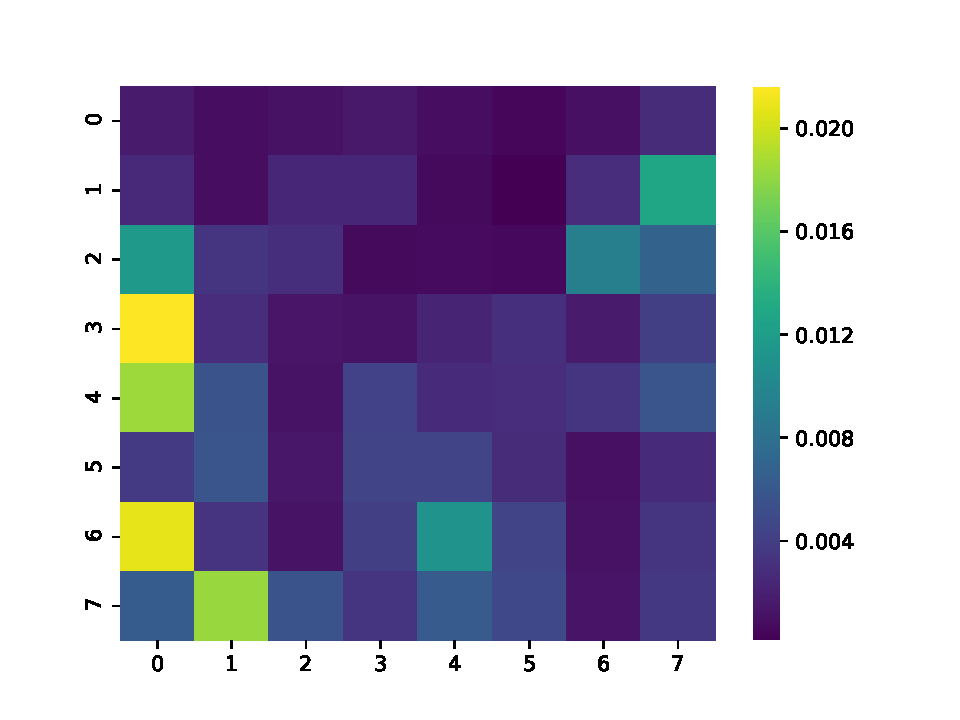
\includegraphics[scale=0.4]{./figures/icu_somvaeprob/detail_heatmaps_unit_discharge_expired_6}
\caption{6-hour mortality risk}
\end{subfigure}
\caption{(a) Dynamic mortality risk in the next 24 hours. (b) Short-term dynamic mortality risk in the next
             6 hours. We observe that the left-edge and right-edge regions of the \texttt{SOMVAEprob} map which
             are enriched for higher acute physiology scores (see Fig \ref{fig:ICU_representations}) also exhibit elevated 
             mortality rates over the baseline. Interestingly, according to future mortality risk, which is an important severity indicator,
             patients on the left-edge are significantly more sick on average than those on the right edge, which is
             less visible from the enrichment for acute physiology scores.}
\end{figure}

\newpage

% Detailed analysis of vital sign abnormalities

\subsubsection*{Patient state phenotypes on the \texttt{SOMVAEprob} map}

\begin{figure}[h!]
\centering
\begin{subfigure}[t]{0.22\textwidth}
\centering
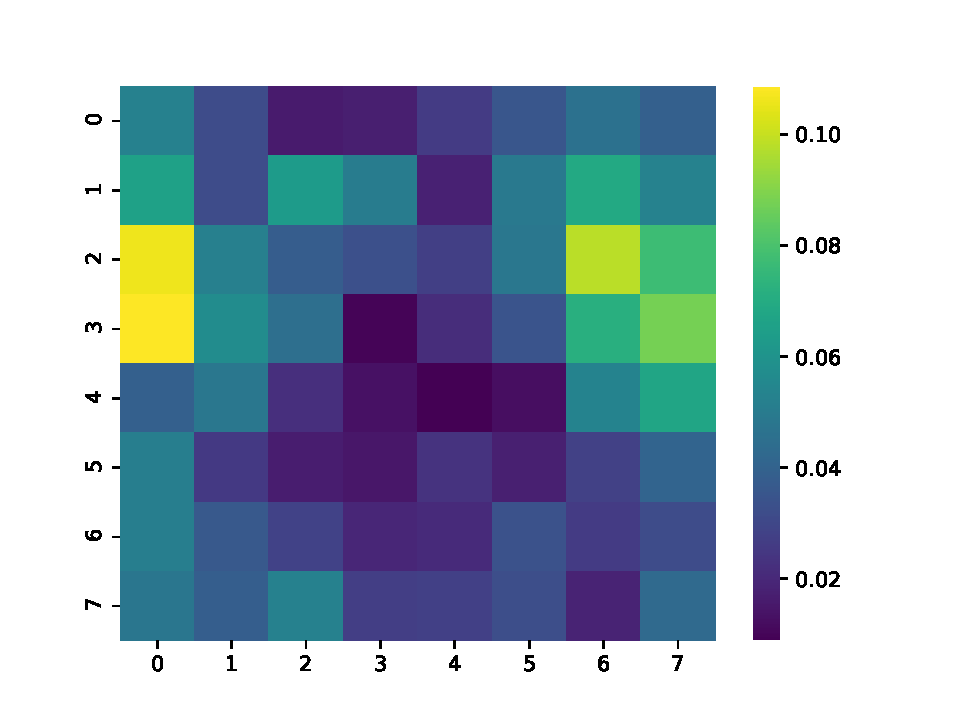
\includegraphics[scale=0.22]{./figures/icu_somvaeprob/detail_heatmaps_low_sodium}
\caption{Low Sodium}
\end{subfigure}
\begin{subfigure}[t]{0.22\textwidth}
\centering
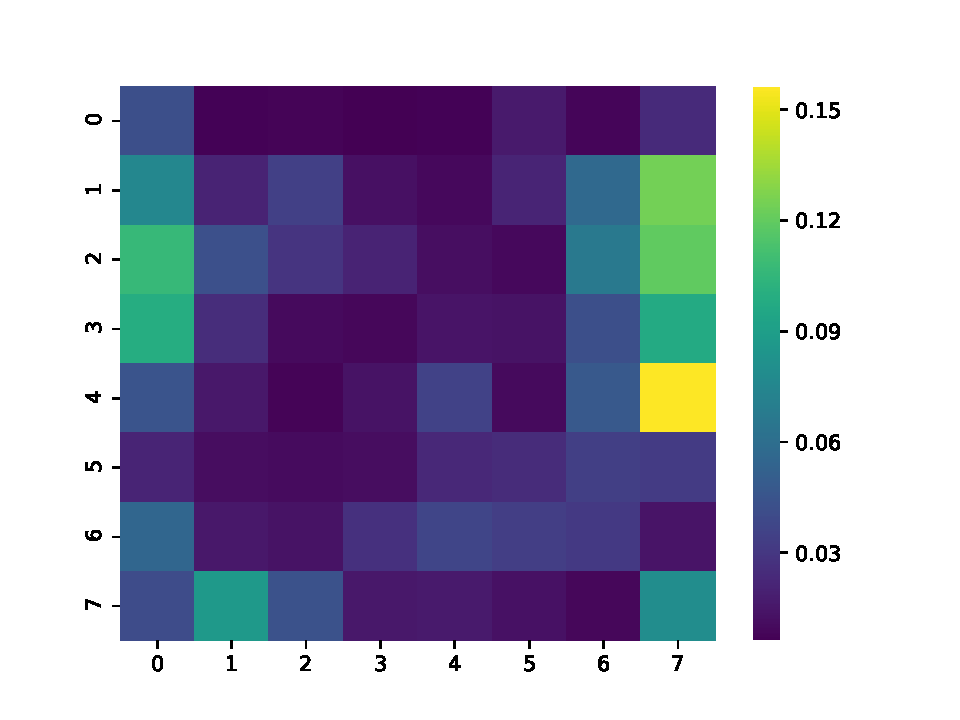
\includegraphics[scale=0.22]{./figures/icu_somvaeprob/detail_heatmaps_high_potassium}
\caption{High Potassium}
\end{subfigure}
\begin{subfigure}[t]{0.22\textwidth}
\centering
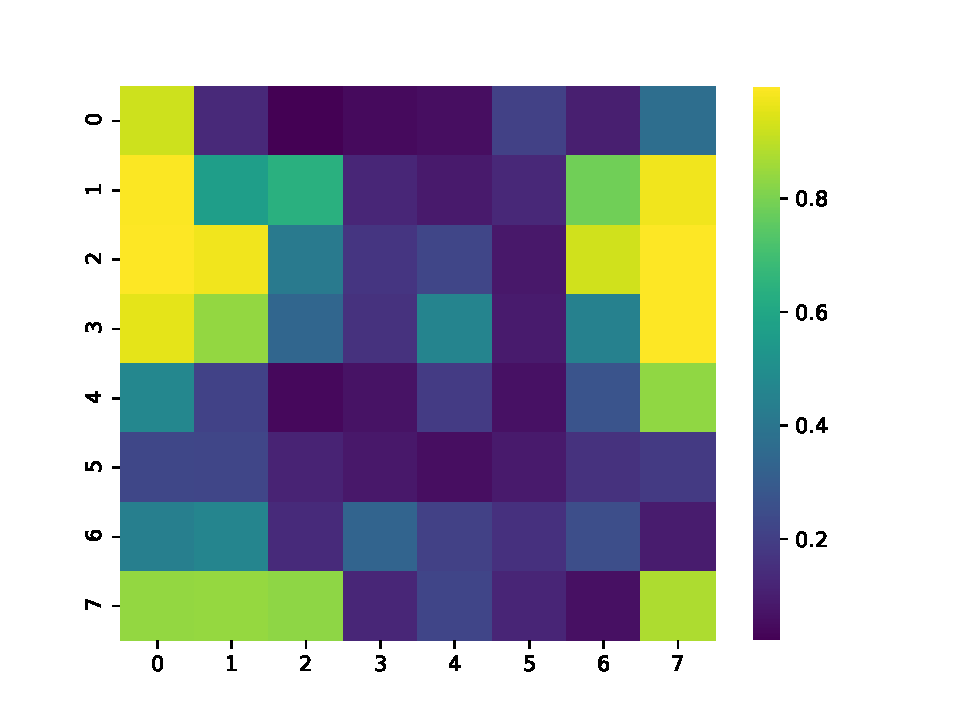
\includegraphics[scale=0.22]{./figures/icu_somvaeprob/detail_heatmaps_high_creatinine}
\caption{High Creatinine}
\end{subfigure}
\begin{subfigure}[t]{0.22\textwidth}
\centering
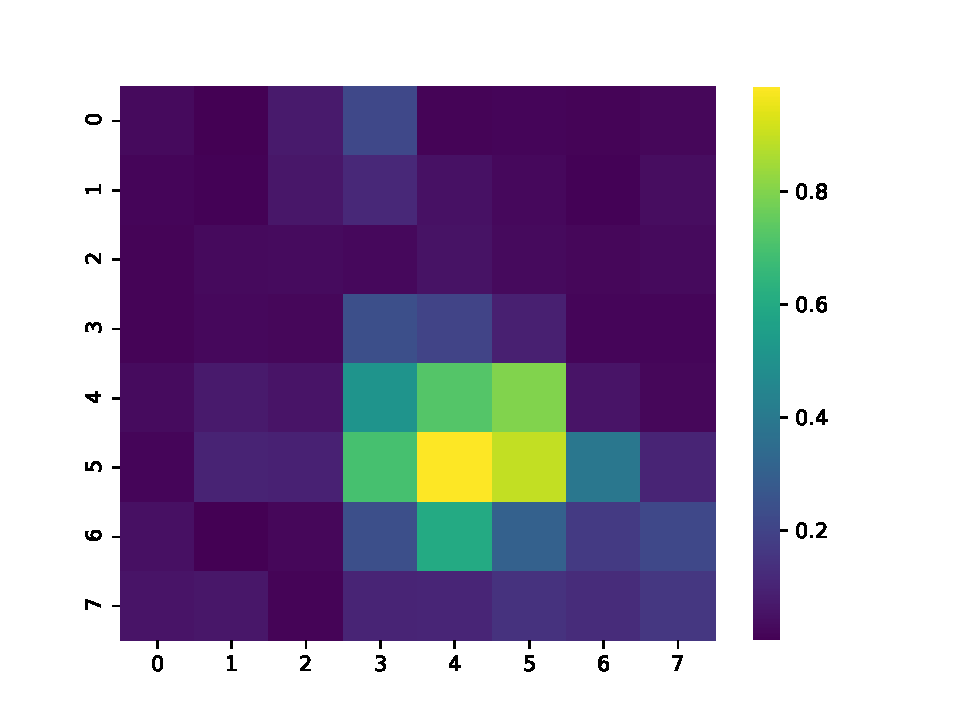
\includegraphics[scale=0.22]{./figures/icu_somvaeprob/detail_heatmaps_high_hco3}
\caption{High HCO3}
\end{subfigure}



\caption{(a) Prevalence of abnormally low sodium lab value in the next 24 
         hours, (b-d) Prevalence of abnormally high potassium/creatinine/HCO3 lab values in the next 24 hours. Each
         sub-figure illustrates the enrichment of a distinct phenotype on the \texttt{SOMVAEprob} map. Low sodium
         and high potassium states are enriched near the left edge, and near the right edge, respectively, which could
         represent sub-types of the high-risk phenotype found in these regions (compare Fig \ref{fig:ICU_representations}
         for the distribution of the acute physiology score). Elevated creatinine is a trait that occurs in both these regions.
         A compact structure associated with elevated HCO3 can be found in the center of the map, which could represent 
         a distinct phenotype with lower mortality risk in our cohort. In all phenotypes, the tendency of \texttt{SOMVAEprob}
         to recover compact structures is exemplified.}
\end{figure}



\begin{figure}[h]
    \centering
    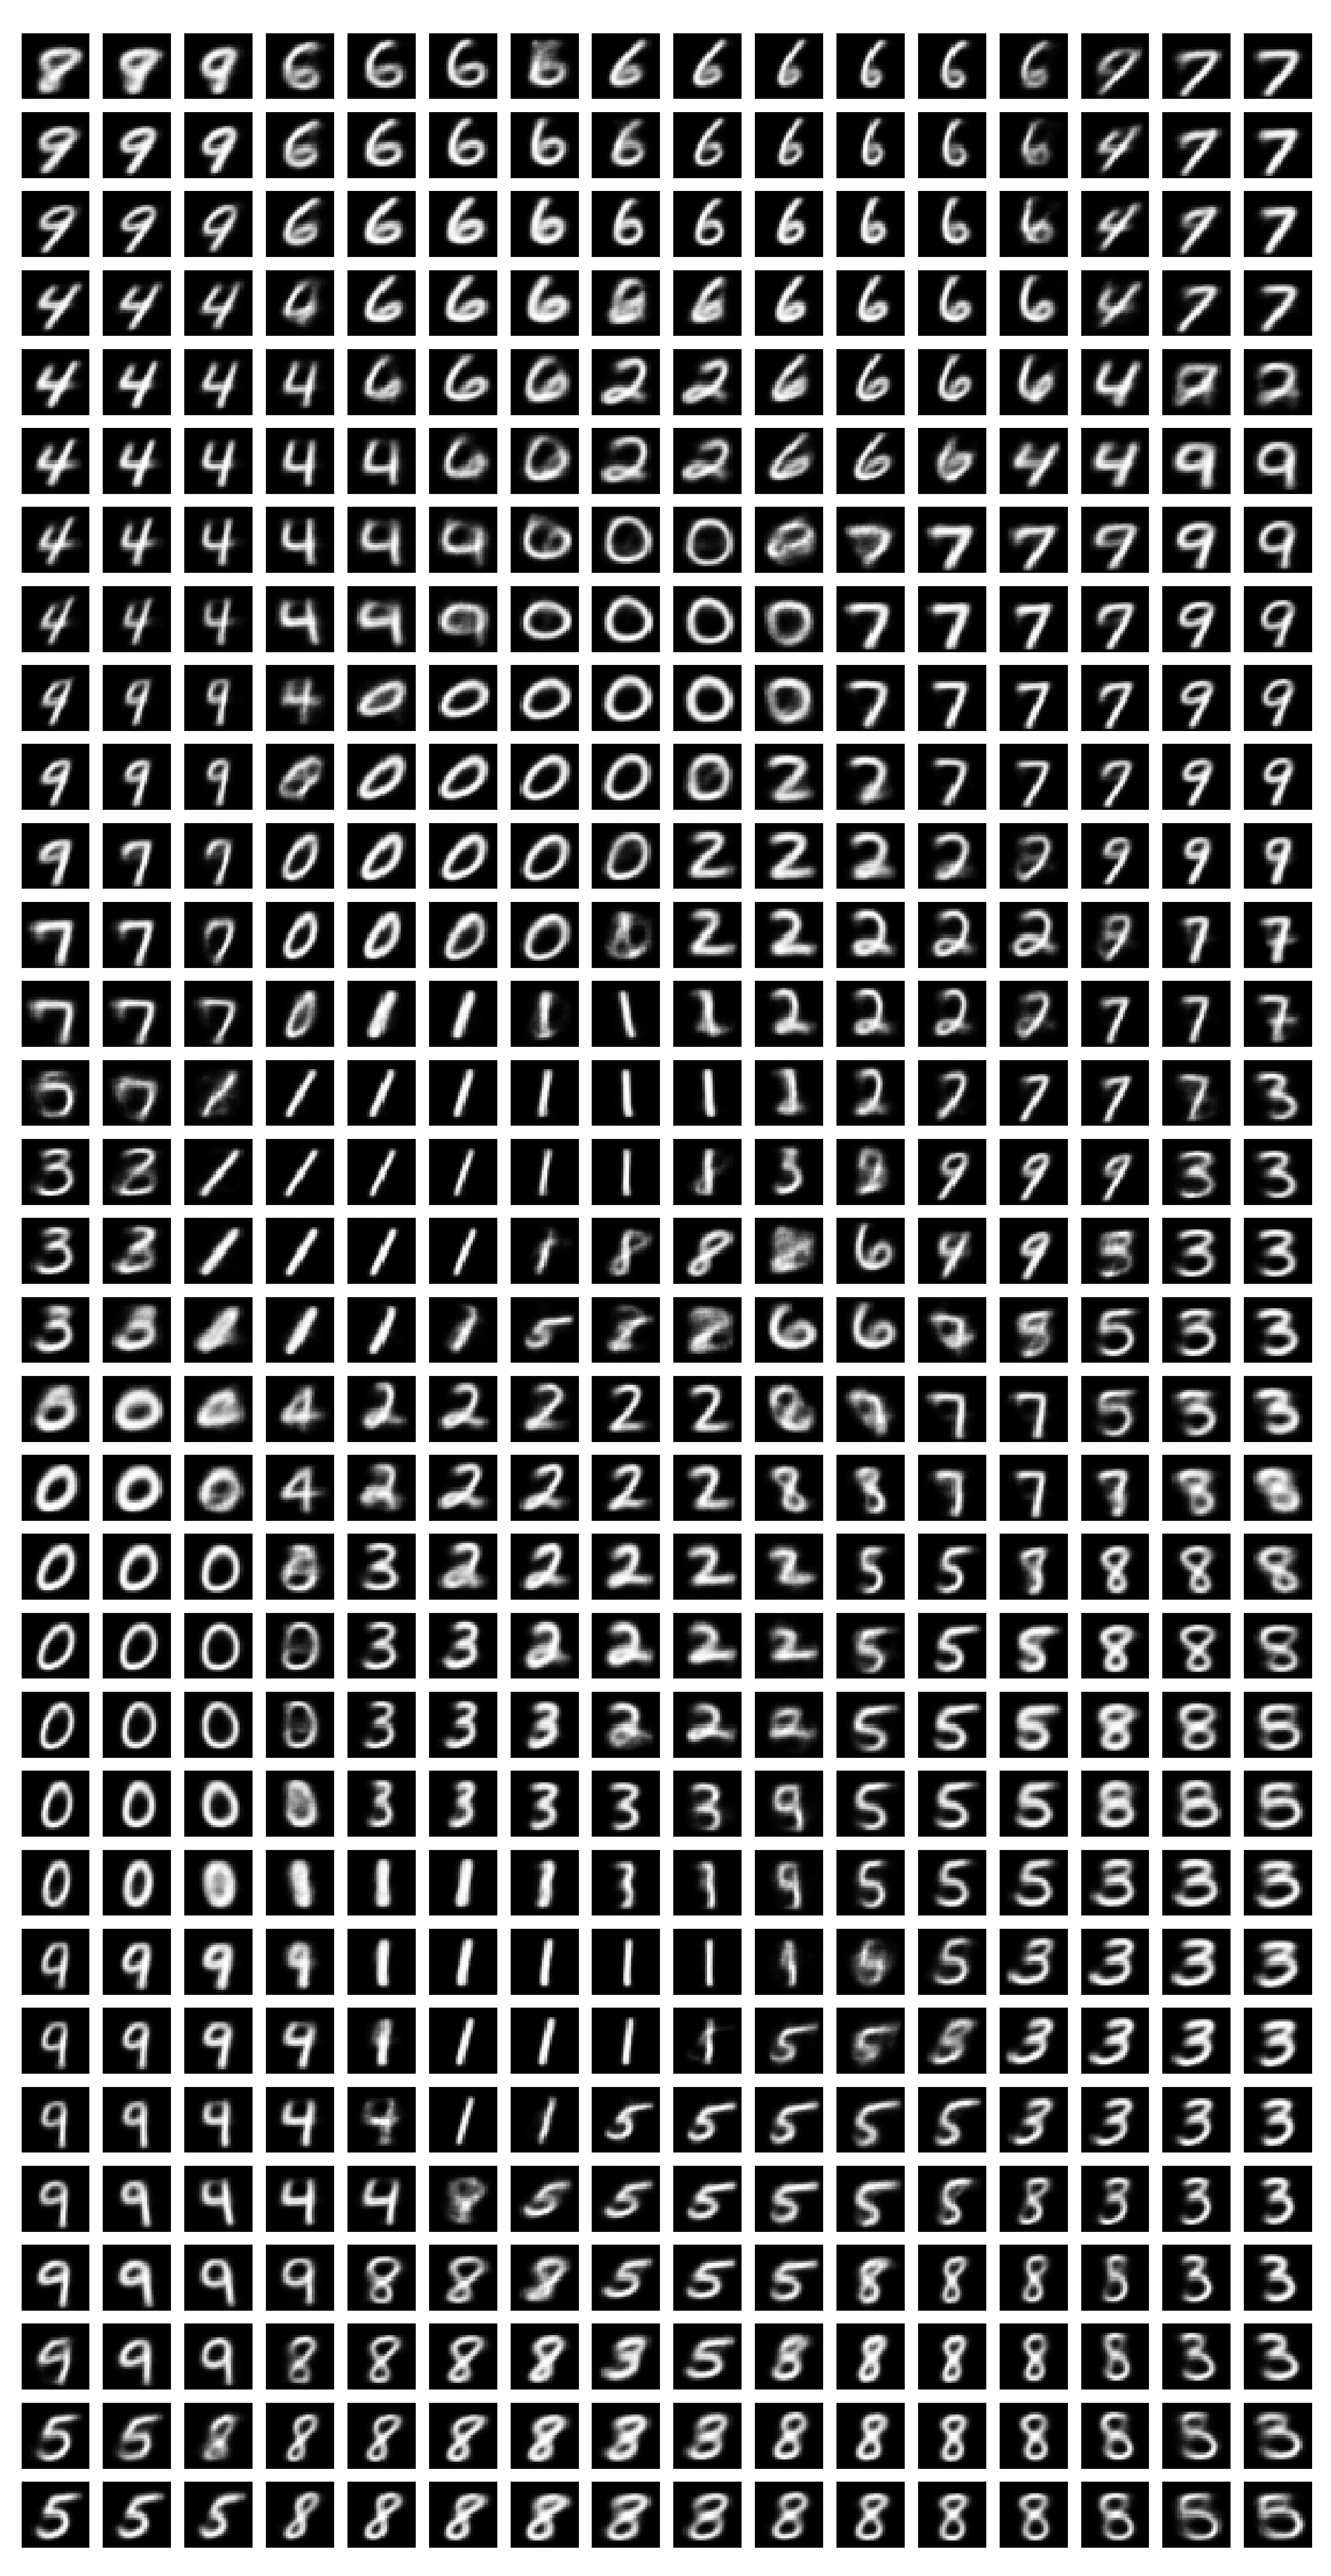
\includegraphics[height=0.8\textheight]{MNIST_SOM.pdf}
    \caption{Images generated from the SOM-VAE's latent space with 512 embeddings trained on MNIST. It yields an interpretable discrete two-dimensional representation of the data manifold in the higher-dimensional latent space.}
    \label{fig:MNIST_SOM}
\end{figure}

\begin{figure}[h]
    \centering
    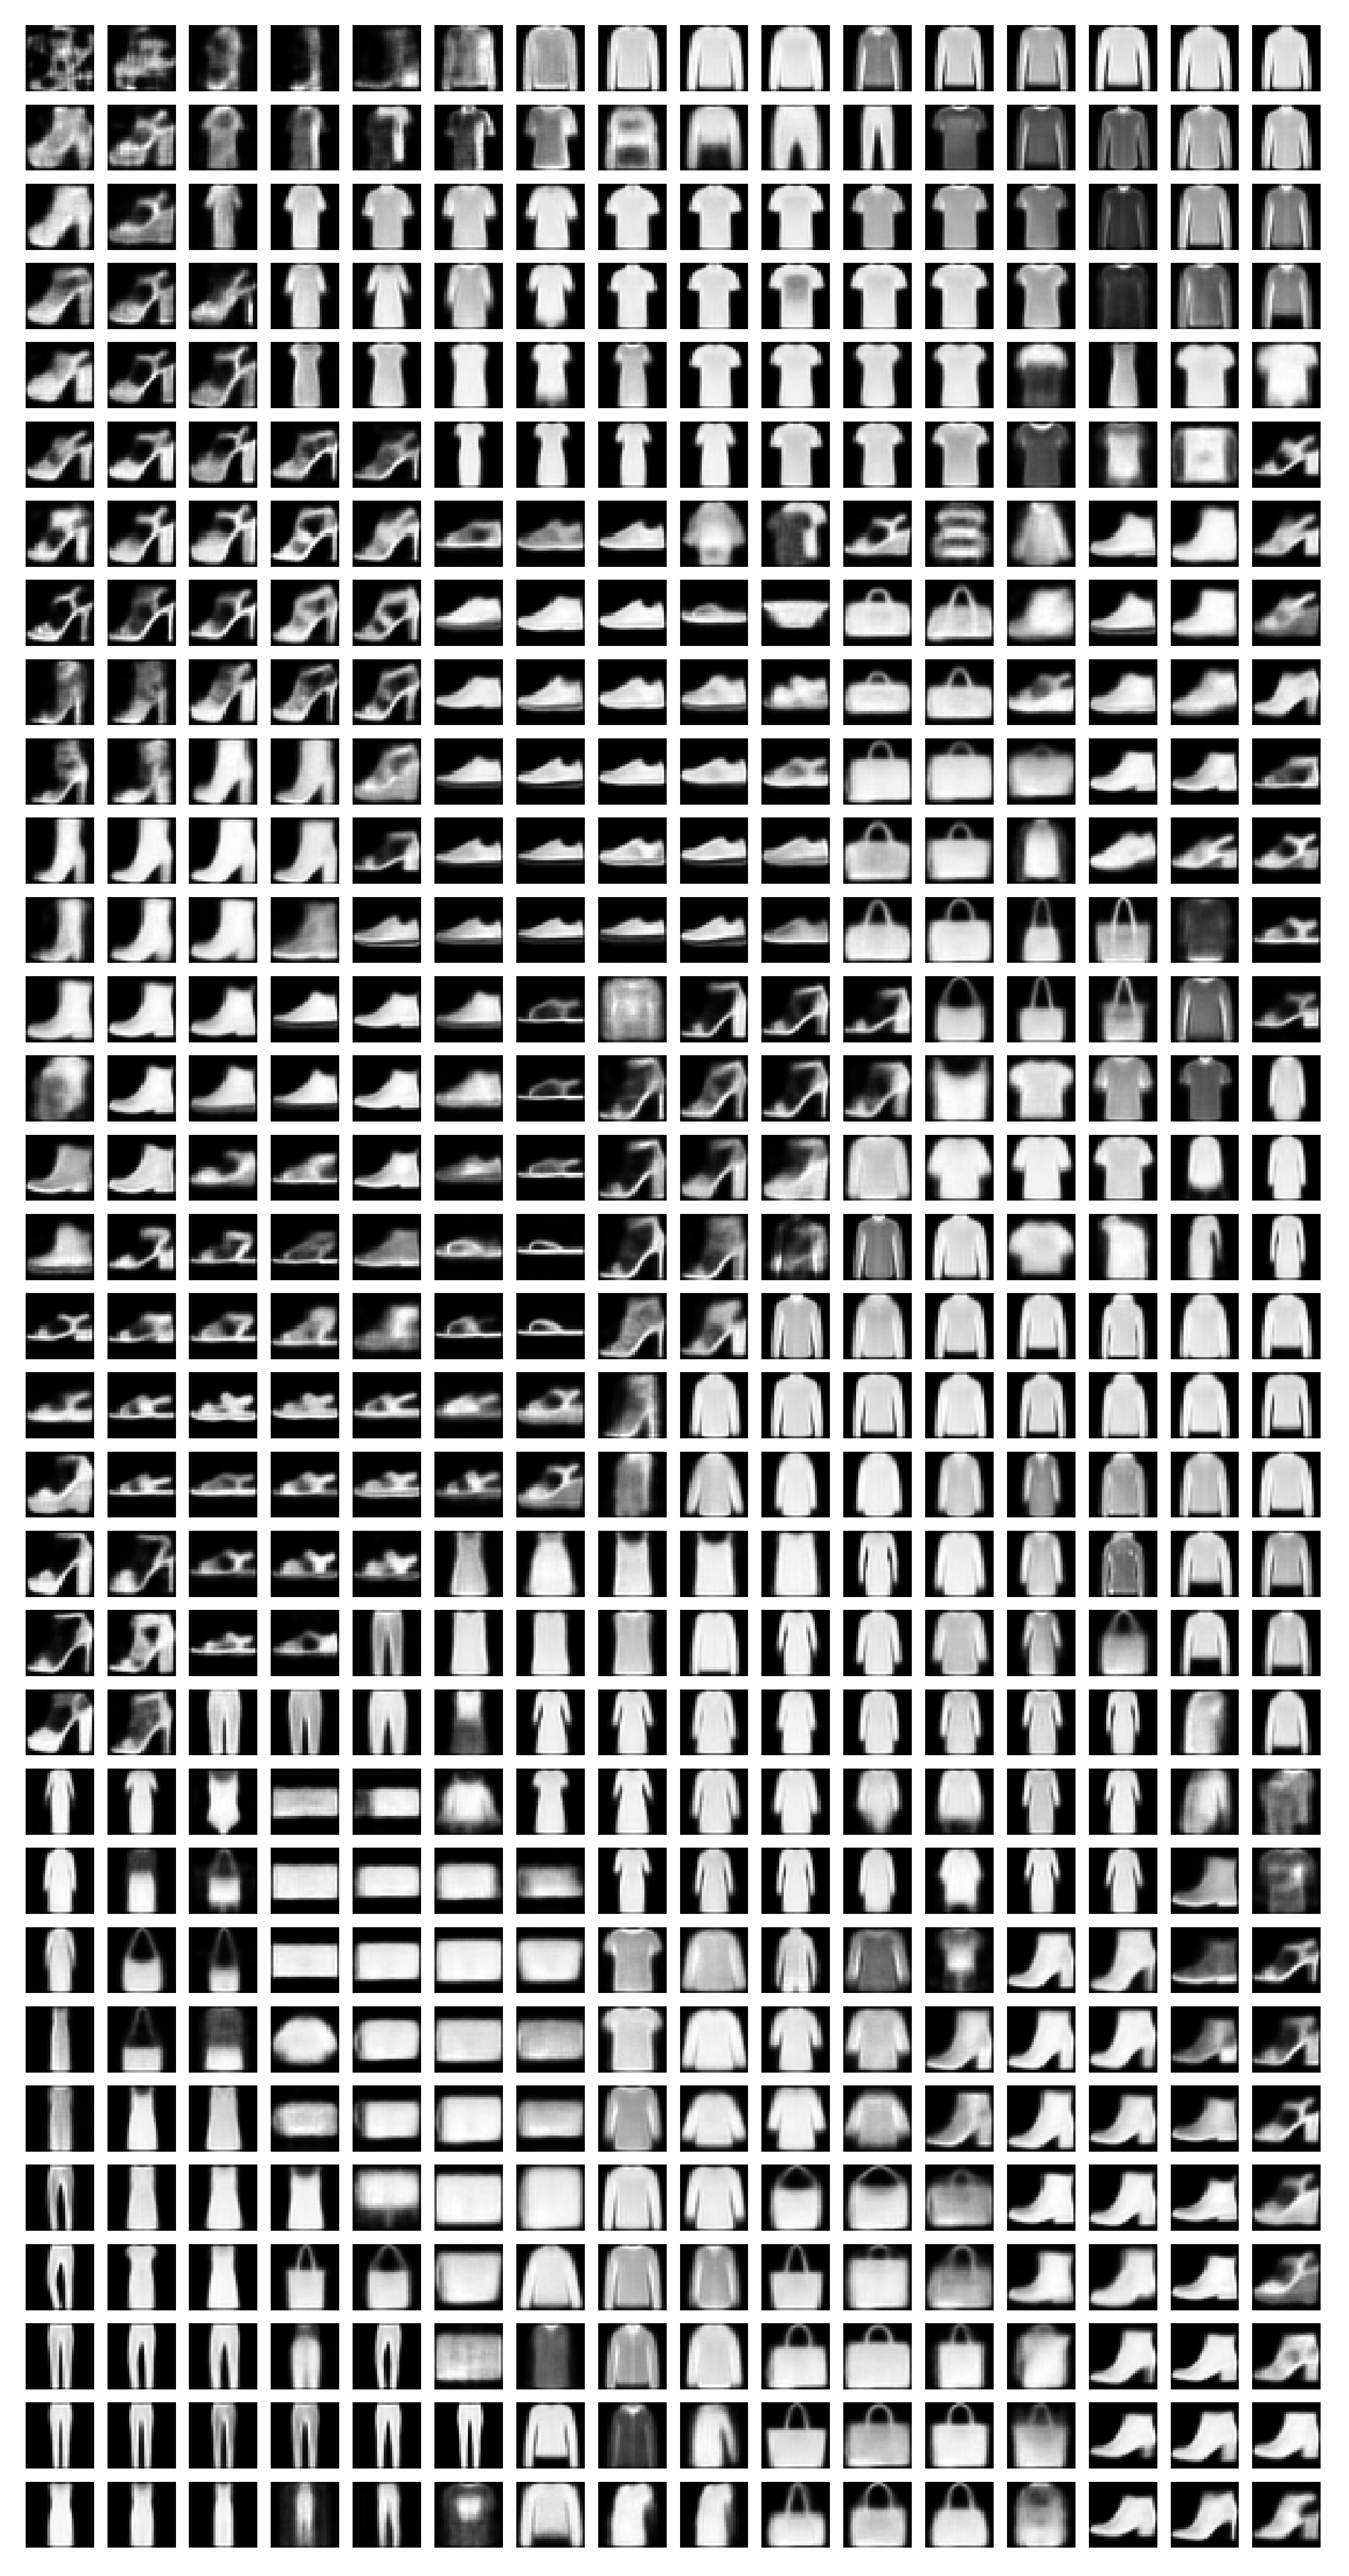
\includegraphics[height=0.8\textheight]{FMNIST_SOM.pdf}
    \caption{Images generated from the SOM-VAE's latent space with 512 embeddings trained on Fashion-MNIST. It yields an interpretable discrete two-dimensional representation of the data manifold in the higher-dimensional latent space.}
    \label{fig:FMNIST_SOM}
\end{figure}






\subsection{Detailed analysis of \texttt{SOMVAEprob} patient states}
\label{subsec:detailed_icu}

As mentioned in the main text (see Fig \ref{fig:ICU_representations}) the \texttt{SOMVAEProb}
is able to uncover compact and interpretable structures in the latent space with respect
to future physiology scores. In this section we show results for acute physiology scores
in greater detail, analyze enrichment for future mortality risk, arguably the most
important severity indicator in the ICU, and explore phenotypes for particular 
physiological abnormalities.

% Acute physiology scores

\subsubsection*{Full results for future acute physiology scores}

\begin{figure}[h!]

\centering
\begin{subfigure}[t]{0.30\textwidth}
\centering
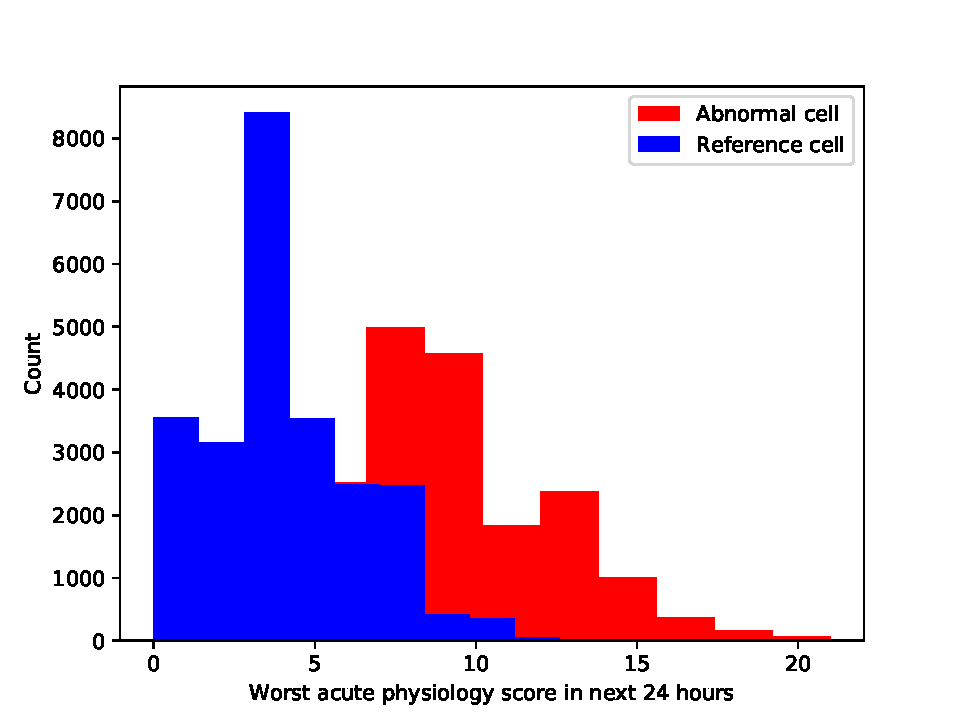
\includegraphics[scale=0.30]{./figures/icu_somvaeprob/distribution_cells}
\caption{Abnormal vs. reference cell}
\end{subfigure}
\begin{subfigure}[t]{0.30\textwidth}
\centering
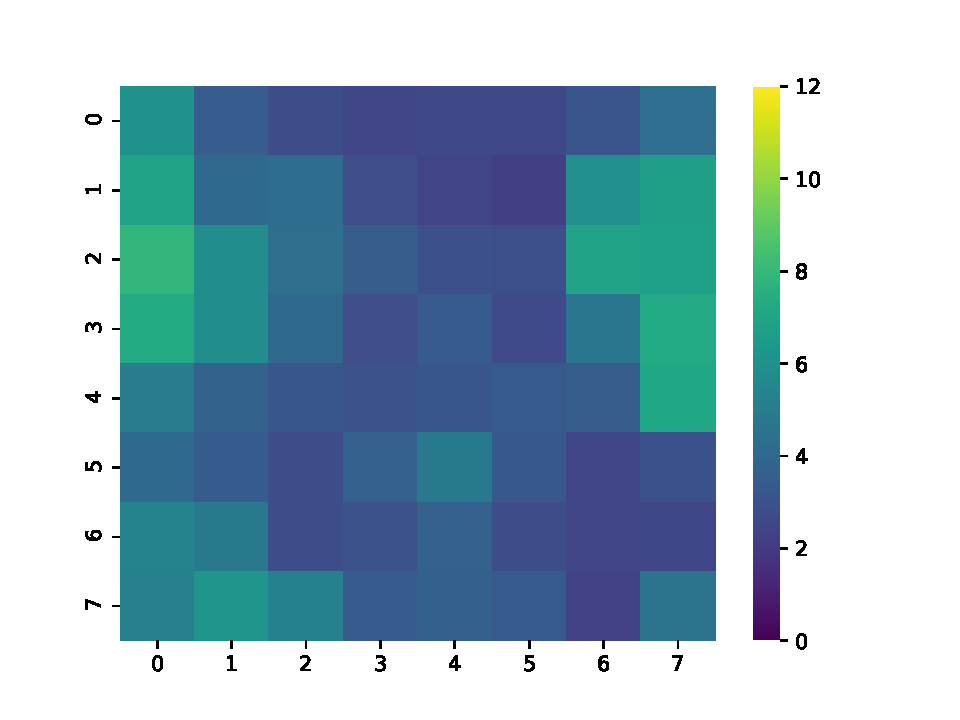
\includegraphics[scale=0.30]{./figures/icu_somvaeprob/detail_heatmaps_full_score_6}
\caption{Acute physiology score (6)}
\end{subfigure}
\begin{subfigure}[t]{0.30\textwidth}
\centering
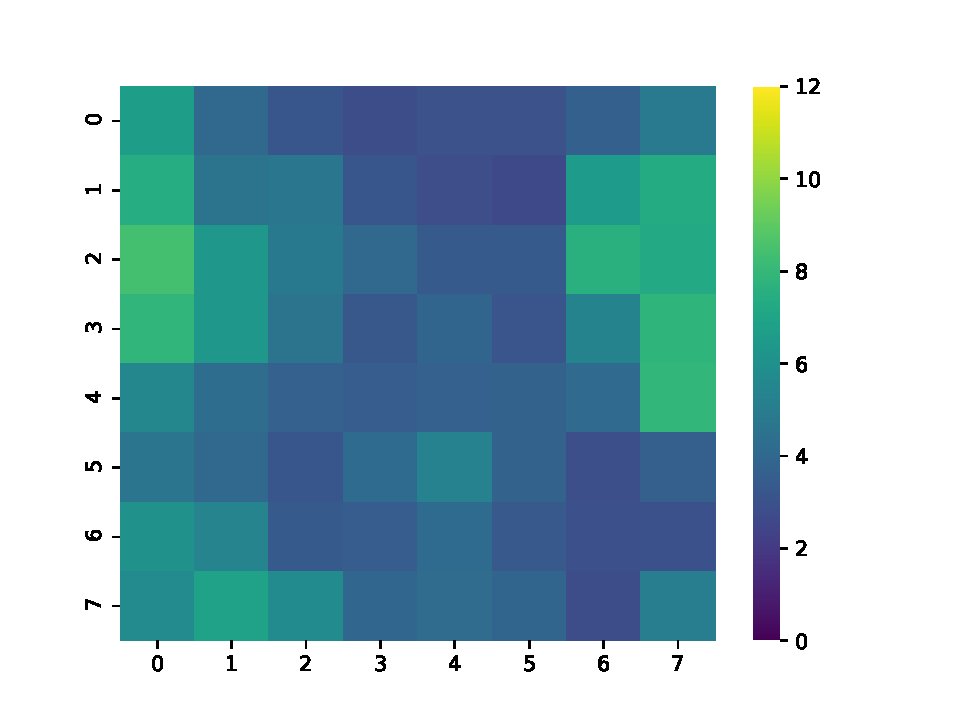
\includegraphics[scale=0.30]{./figures/icu_somvaeprob/detail_heatmaps_full_score_12}
\caption{ Acute physiology score (12)}
\end{subfigure}

\caption{(a) shows the difference in distribution of the acute
         physiology score in the next 24 hours, between time-points assigned to the most 
         abnormal cell in the \texttt{SOMVAEprob} map with coordinates [2,0] vs. 
         a normal cell chosen from the middle of the map with coordinates [4,3]. It is apparent that
         the distributions are largely disjoint, which means that the representation induced by 
         \texttt{SOMVAEprob} clearly distinguishes these risk profiles. Statistical tests for difference
         in distribution and location parameter are highly significant at p-values of $p \leq 10^{-3}$, as we
         have validated using a 2-sample $t$-test and Kolmogorov-Smirnov test. In (b-c) the enrichment 
         of the map for the mean acute physiology score in the next 6 and 12 hours is shown, for completeness.
         The enrichment patterns on the 3 maps, for the future horizons $\{6,12,24\}$, are almost identical, 
         which provides empirical evidence for the temporal stability of the \texttt{SOMVAEProb} embedding.}

\end{figure}

% Dynamic mortality in the next {12,24} hours

\subsubsection*{Dynamic mortality risk of patients on the \texttt{SOMVAEprob} map}

\begin{figure}[h!]
\centering
\begin{subfigure}[t]{0.47\textwidth}
\centering
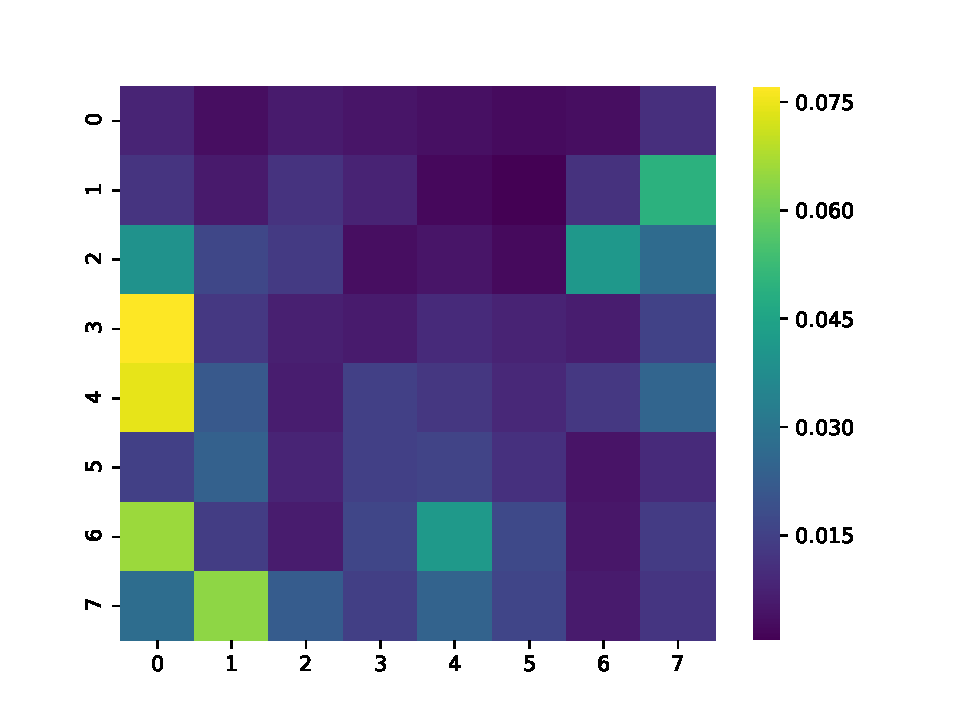
\includegraphics[scale=0.4]{./figures/icu_somvaeprob/detail_heatmaps_unit_discharge_expired_24}
\caption{24-hour mortality risk}
\end{subfigure}
\begin{subfigure}[t]{0.47\textwidth}
\centering
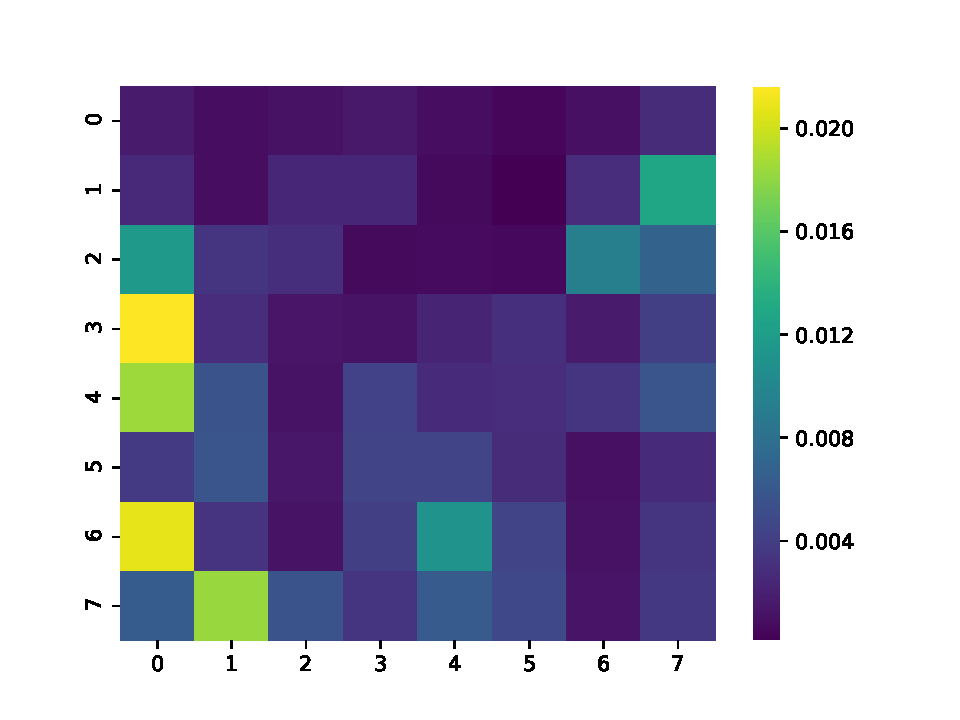
\includegraphics[scale=0.4]{./figures/icu_somvaeprob/detail_heatmaps_unit_discharge_expired_6}
\caption{6-hour mortality risk}
\end{subfigure}
\caption{(a) Dynamic mortality risk in the next 24 hours. (b) Short-term dynamic mortality risk in the next
             6 hours. We observe that the left-edge and right-edge regions of the \texttt{SOMVAEprob} map which
             are enriched for higher acute physiology scores (see Fig \ref{fig:ICU_representations}) also exhibit elevated 
             mortality rates over the baseline. Interestingly, according to future mortality risk, which is an important severity indicator,
             patients on the left-edge are significantly more sick on average than those on the right edge, which is
             less visible from the enrichment for acute physiology scores.}
\end{figure}

\newpage

% Detailed analysis of vital sign abnormalities

\subsubsection*{Patient state phenotypes on the \texttt{SOMVAEprob} map}

\begin{figure}[h!]
\centering
\begin{subfigure}[t]{0.22\textwidth}
\centering
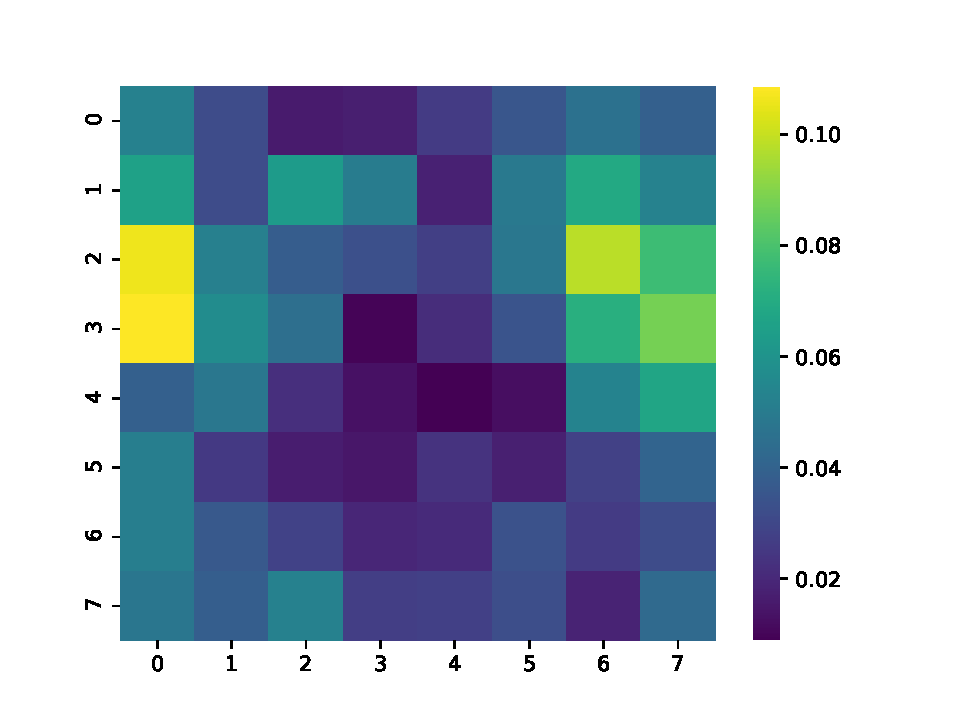
\includegraphics[scale=0.22]{./figures/icu_somvaeprob/detail_heatmaps_low_sodium}
\caption{Low Sodium}
\end{subfigure}
\begin{subfigure}[t]{0.22\textwidth}
\centering
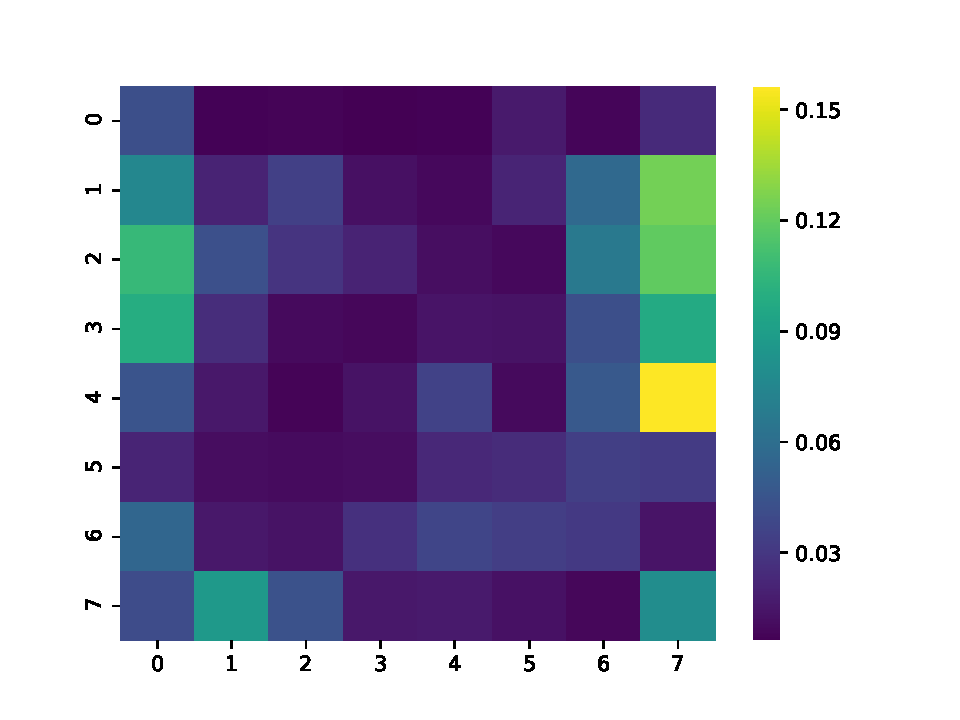
\includegraphics[scale=0.22]{./figures/icu_somvaeprob/detail_heatmaps_high_potassium}
\caption{High Potassium}
\end{subfigure}
\begin{subfigure}[t]{0.22\textwidth}
\centering
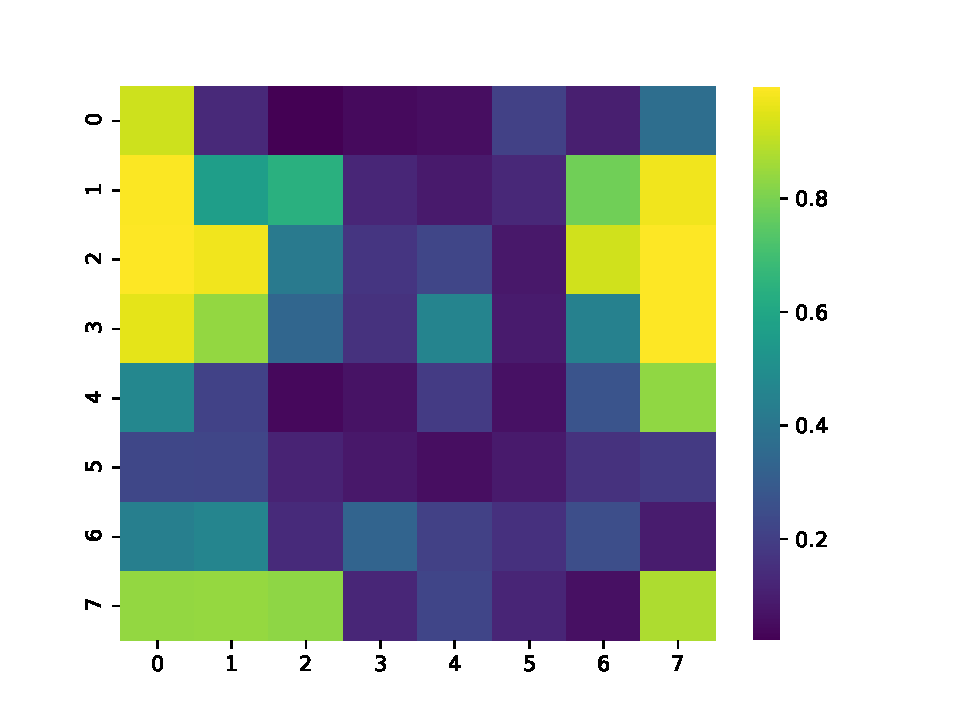
\includegraphics[scale=0.22]{./figures/icu_somvaeprob/detail_heatmaps_high_creatinine}
\caption{High Creatinine}
\end{subfigure}
\begin{subfigure}[t]{0.22\textwidth}
\centering
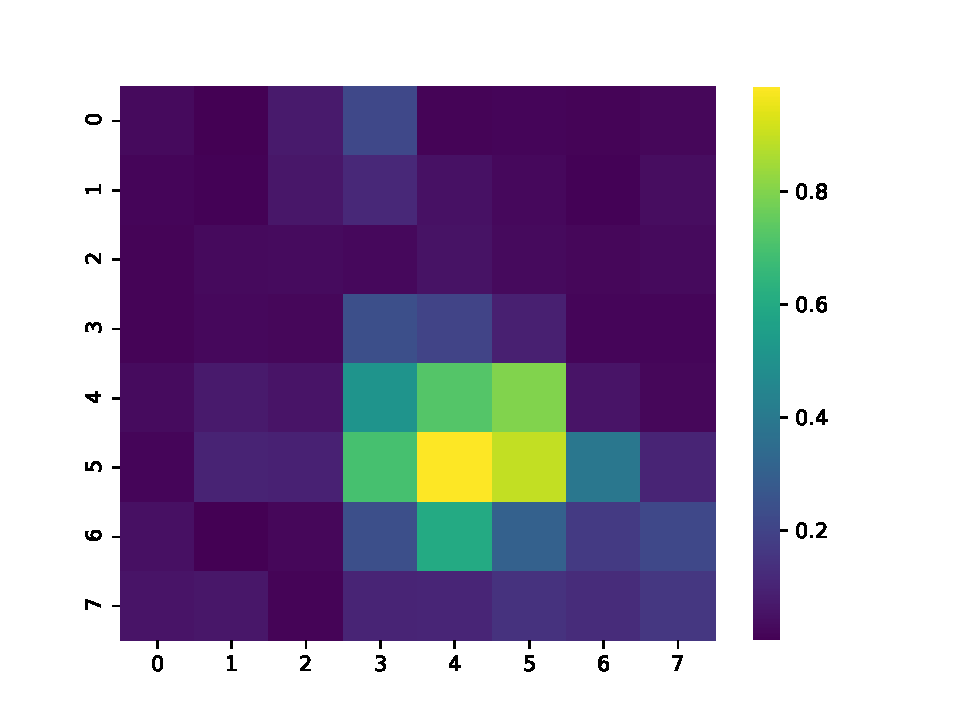
\includegraphics[scale=0.22]{./figures/icu_somvaeprob/detail_heatmaps_high_hco3}
\caption{High HCO3}
\end{subfigure}



\caption{(a) Prevalence of abnormally low sodium lab value in the next 24 
         hours, (b-d) Prevalence of abnormally high potassium/creatinine/HCO3 lab values in the next 24 hours. Each
         sub-figure illustrates the enrichment of a distinct phenotype on the \texttt{SOMVAEprob} map. Low sodium
         and high potassium states are enriched near the left edge, and near the right edge, respectively, which could
         represent sub-types of the high-risk phenotype found in these regions (compare Fig \ref{fig:ICU_representations}
         for the distribution of the acute physiology score). Elevated creatinine is a trait that occurs in both these regions.
         A compact structure associated with elevated HCO3 can be found in the center of the map, which could represent 
         a distinct phenotype with lower mortality risk in our cohort. In all phenotypes, the tendency of \texttt{SOMVAEprob}
         to recover compact structures is exemplified.}
\end{figure}

\begin{abstract}


High-dimensional time series are common in many domains.
Since human cognition is not optimized to work well in high-dimensional spaces, these areas could benefit from interpretable low-dimensional representations.
However, most representation learning algorithms for time series data are difficult to interpret.
This is due to non-intuitive mappings from data features to salient properties of the representation and non-smoothness over time.

To address this problem, we propose a new representation learning framework building on ideas from interpretable discrete dimensionality reduction and deep generative modeling.
This framework allows us to learn discrete representations of time series, which give rise to smooth and interpretable embeddings with superior clustering performance.
We introduce a new way to overcome the non-differentiability in discrete representation learning and present a gradient-based version of the traditional self-organizing map algorithm that is more performant than the original.
Furthermore, to allow for a probabilistic interpretation of our method, we integrate a Markov model in the representation space.
This model uncovers the temporal transition structure, improves clustering performance even further and provides additional explanatory insights as well as a natural representation of uncertainty.

We evaluate our model in terms of clustering performance and interpretability on static (Fashion-)MNIST data, a time series of linearly interpolated (Fashion-)MNIST images, a chaotic Lorenz attractor system with two macro states, as well as on a challenging real world medical time series application on the eICU data set.
Our learned representations compare favorably with competitor methods and facilitate downstream tasks on the real world data.

\end{abstract}

\pdfoutput=1
\documentclass{article}
\usepackage{iclr2019_conference,times}


%-------------------------------------------------------------- Includes

\usepackage{bbm}  % who knows?

\usepackage{amsmath}          % basic math
\usepackage{amssymb} 			    % math symbols
% \usepackage{amsthm}           % theorems
\usepackage{textcomp}

% \usepackage{float}            % make figures work
% \usepackage{cite}             % citations would be nice
\usepackage{url}              % better urls; magically keeping doc from breaking due to urls in refs

% \usepackage{tabu}
\usepackage{array}            % multiline table cells; somehow
\usepackage{tabularx}         % better tables
% \usepackage[table]{xcolor}    % colored table cells  % incompatible with sigconf
\usepackage{colortbl}
\newcolumntype{Y}{>{\centering\arraybackslash}X}	% centered column type for tabularx

% stuff for piecewise functions
\usepackage{mathtools}          %loads amsmath as well
\DeclarePairedDelimiter\Floor\lfloor\rfloor
\DeclarePairedDelimiter\Ceil\lceil\rceil

% \DeclareMathOperator*{\argmin}{arg\,min} % argmin
% \DeclareMathOperator*{\argmax}{arg\,max} % argmax
\DeclareMathOperator*{\argmin}{argmin} % argmin
\DeclareMathOperator*{\argmax}{argmax} % argmax

\usepackage{pbox}   % for trick to force linebreaks in table cells

\usepackage{setspace}
% \usepackage{setspace}

% \usepackage{booktabs} % acm recommended, and for pandas latex tables

%-------------------------------------------------------------- Algorithm setup

% commented out for sysml

% \usepackage{algorithm}
% \usepackage[noend]{algpseudocode} % I think this removes trailing "end {if,for,while}"

% % \algnewcommand{\LineComment}[1]{\State \(\triangleright\) #1} % left-aligned comments
% % \algnewcommand{\SideComment}[1]{\(//\) #1}
% \algnewcommand{\COMMENT}[2][.5\linewidth]{\leavevmode\hfill\makebox[#1][l]{//~#2}}
% \algnewcommand{\LineComment}[1]{\State \(//\) #1}	% left-aligned comments
% \algnewcommand\RETURN{\State \textbf{return} }


%-------------------------------------------------------------- Figures setup

% \usepackage[pdftex]{graphicx}
\usepackage{graphicx}
\usepackage[space]{grffile}   % allow spaces in file names
% declare the path(s) where your graphic files are
% \graphicspath{{../figs/survey/}}
\graphicspath{{./figs/}}
% and their extensions so you won't have to specify these
\DeclareGraphicsExtensions{.pdf,.jpeg,.jpg,.png}


%\textfloatsep: space between last top float or first bottom float and the text (default = 20.0pt plus 2.0pt minus 4.0pt).
%\intextsep : space left on top and bottom of an in-text float (default = 12.0pt plus 2.0pt minus 2.0pt).
\setlength{\textfloatsep}{4pt}
\setlength{\intextsep}{4pt}

% \usepackage{caption}
% \usepackage[font={small,it}]{caption}
\usepackage[font={bf}]{caption}
\setlength{\abovecaptionskip}{1pt} % less space between captions and figures
% \setlength{\abovecaptionskip}{-2pt} % less space between captions and figures
% \setlength{\abovecaptionskip}{-5pt}	% less space between captions and figures
% \setlength{\belowcaptionskip}{-13pt}  % less space below captions
% \setlength{\belowcaptionskip}{-10pt}  % less space below captions
\setlength{\belowcaptionskip}{-4pt}	% less space below captions

% \usepackage{paralist}
% \setdefaultleftmargin{10pt}{10pt}{}{}{}{}

% \usepackage{changepage}
% \usepackage{tabulary}

\usepackage{outlines}
\usepackage{enumitem}
\newcommand{\ItemSpacing}{0mm}
\newcommand{\ParSpacing}{0mm}
\setenumerate[1]{itemsep={\ItemSpacing},parsep={\ParSpacing},label=\arabic*.}
% \setenumerate[2]{itemsep={\ItemSpacing},parsep={\ParSpacing},label=\arabic*.}
\setenumerate[2]{itemsep={\ItemSpacing},parsep={\ParSpacing}}

% \usepackage[linewidth=1pt]{mdframed}
% \mdfsetup{frametitlealignment=\center, skipabove=0, innertopmargin=1mm,
% innerleftmargin=2mm, leftmargin=0mm, rightmargin=0mm}

%-------------------------------------------------------------- Miscellaneous setup

% \usepackage{enumitem}
% \setlist{nolistsep}
% \setlist{first=itemsep1em}
% \setlist[1]{labelindent=\parindent}

% \newlength\myindent
% \setlength\myindent{2em}
% \newcommand\bindent{%
%   \begingroup
%   \setlength{\itemindent}{\myindent}
%   \addtolength{\algorithmicindent}{\myindent}
% }
% \newcommand\eindent{\endgroup}

% remove unwanted space between paragraphs;
% it's set by the IEEE conference format, but no papers from this conference have it
% \parskip 0ex plus 0.2ex minus 0.1ex

% make vectors be bold instead of with arrows
\renewcommand{\vec}[1]{\mathbf{#1}}
% add 'mat' command to make matrices bold
\newcommand{\mat}[1]{\mathbf{#1}}

\DeclarePairedDelimiter\ceil{\lceil}{\rceil}
\DeclarePairedDelimiter\floor{\lfloor}{\rfloor}

\newtheorem{Definition}{Definition}[section]

% ------------------------ convenience commands
\newcommand\eps\varepsilon
\DeclareMathOperator{\infimum}{inf}
\renewcommand\inf\infty
\DeclareMathOperator{\erfc}{erfc}

\renewcommand{\c}{\vec{c}}
\newcommand{\q}{\vec{q}}
\renewcommand{\r}{\vec{r}}
\renewcommand{\v}{\vec{v}}
\newcommand{\vhat}{\hat{\vec{v}}}
\newcommand{\x}{\vec{x}}
\newcommand{\xhat}{\hat{\vec{x}}}
\newcommand{\y}{\vec{y}}
\newcommand{\yhat}{\hat{\vec{y}}}
\newcommand{\z}{\vec{z}}
\newcommand{\zhat}{\hat{\vec{z}}}

\newcommand{\lam}{\lambda}
\newcommand{\sig}{\sigma}
\newcommand{\Sig}{\Sigma}

\newcommand{\E}{\mathop{{}\mathbb{E}}}

\renewcommand{\H}{\mathcal{H}}
\newcommand{\R}{\mathbb{R}}
\newcommand{\V}{\mathcal{V}}
\newcommand{\Xs}{\mathcal{X}}
\newcommand{\Z}{\mathcal{Z}}
\renewcommand{\S}{\mathcal{S}}
\newcommand{\Nb}{\mathcal{N}_b}

\newcommand{\onehalf}{\frac{1}{2}}

\newcommand{\Xcal}{\mathcal{X}}
\newcommand{\Ycal}{\mathcal{Y}}

\newcommand{\pie}[1]{\frac{\pi}{#1}}
% \newcommand{\pitwo}{\frac{\pi}{2}}
% \newcommand{\pifour}{\frac{\pi}{4}}

% \newcommand{\norm}[1]{\left\lVert #1 \right\rVert}
\DeclarePairedDelimiter\abs{\lvert}{\rvert}%
\DeclarePairedDelimiter\norm{\lVert}{\rVert}%

\DeclareMathOperator{\Beta}{Beta}
\DeclareMathOperator{\Normal}{\mathcal{N}}
\DeclareMathOperator{\erf}{erf}
\DeclareMathOperator{\Var}{Var}

% make *all* text 10pt
% \renewcommand{\footnotesize}{\normalsize}
% \renewcommand{\footnotesize}{\small}
% \renewcommand{\small}{\normalsize}

% ------------------------------------------------ stuff that might break things


% \usepackage{mathtools}
% \usepackage{amsthm}           % theorems
% \newtheorem{theorem}{Theorem}[section]
% \newtheorem{lemma}{Lemma}[section]
% \newtheorem{definition}{Definition}[section]
% \newtheorem{corollary}{Corrolary}[section]


\title{SOM-VAE: Interpretable Discrete Representation Learning on Time Series}


\author{Vincent Fortuin, Matthias H\"user \& Francesco Locatello  \\
Department of Computer Science, ETH Z\"urich \\
Universit\"atsstrasse 6, 8092 Z\"urich, Switzerland \\
\texttt{\{fortuin, mhueser, locatelf\}@inf.ethz.ch} \\
\AND
Heiko Strathmann \\
Gatsby Unit, University College London \\
25 Howland Street, London W1T 4JG, United Kingdom \\
\texttt{heiko.strathmann@gmail.com} \\
\AND
Gunnar R\"atsch \\
Department of Computer Science, ETH Z\"urich \\
Universit\"atsstrasse 6, 8092 Z\"urich, Switzerland \\
\texttt{raetsch@inf.ethz.ch}
}



\date{}

\iclrfinalcopy

\begin{document}

\maketitle

	
\begin{abstract}

Continuous Integration (CI) is a software development practice that builds and tests software frequently (e.g., at every push). One main motivator to adopt CI is the potential to deliver software functionalities more quickly than not using CI. However, there is little empirical evidence to support that CI helps projects deliver software functionalities more quickly. Through the analysis of 162,653 pull requests (PRs) of 87 GitHub projects, we empirically study whether adopting a CI service (\textsc{TravisCI}) can quicken the time to deliver merged PRs. 
We complement our quantitative study by analyzing 450 survey responses from participants of 73 software projects.
Our results reveal that adopting a CI service may not necessarily quicken the delivery of merge PRs. Instead, the pivotal benefit of a CI service is to improve the decision making on PR submissions, without compromising the quality or overloading the project's reviewers and maintainers. The automation provided by CI and the boost in developers' confidence are key advantages of adopting a CI service. Furthermore, open-source projects planning to attract and retain developers should consider the use of a CI service in their project, since CI is perceived to lower the contribution barrier while making contributors feel more confident and engaged in the project.
		
\keywords{Continuous Integration \and Pull Request \and Delivery Time \and Code Review}
 
\end{abstract}


\section{Introduction}
\label{sec:introduction}
Before the early 1960s, it was believed that $CP$ is a good symmetry of nature. As Landau pointed out, that would make it impossible for particles to have electric dipole moments (EDMs) along their spin axis \cite{landau1957conservation}. The detection of such an EDM would thus provide clear evidence of $CP$-violation (CPV).  \blfootnote{*Present address: JILA, National Institute of Standards and Technology and University of
Colorado, and Department of Physics, Boulder, Colorado 80309, USA}

While most processes preserve $CP$, certain weak interactions violate it as observed in $K$-, $B$-, and $D$-meson decays \cite{christenson1964evidence, PDG18}. The flavor-changing part of the Standard Model (SM) quark sector includes a CPV phase in the CKM quark-mixing matrix \cite{peccei1995}. This so-called Kobayashi-Maskawa mechanism introduces the third quark generation to explain the CPV \cite{kobayashi1973cp}. The CKM phase has been the only source of observed CPV so far~\cite{PDG18}.

A major motivation for CPV searches comes from the baryon asymmetry of the universe (BAU). Compared to the current baryon density $n_{\text{B}}$, the antibaryon density $n_{\overline{\text{B}}}$ is very small; the reported upper bounds for the antimatter-to-matter number ratio range from $10^{-15}$ to $10^{-6}$ \cite{canetti2012matter}. To date, no mechanism has been experimentally verified that can explain the BAU. In a 1967 paper, Sakharov argued that CPV is necessary to explain the BAU \cite{sakharov1991violation} if the initial conditions of the universe were $C$-symmetric. The existing CPV in the CKM matrix is not enough to explain the extent of the BAU \cite{pospelov2005electric}. Thus new sources of CPV are required to explain the BAU.

No flavor-neutral CPV signal has been observed yet. However, many mechanisms can lead to such phenomena. For example, the QCD Lagrangian can, in principle, include an effective CPV term, proportional to the parameter $\bar{\theta}$~\cite{pospelov1999theta}:
\begin{equation}
	\mathcal{L} = \bar{\theta}\frac{g^2}{32\pi^2}G^a_{\mu\nu}\widetilde{G}^a_{\mu\nu},
\end{equation}
where $G^a$ is the gluon field tensor, $g$ is the strong coupling constant, and $\bar{\theta}$ is dimensionless. Experimental limits from experiments searching for CPV in neutral $^{199}$Hg atoms \cite{graner2016reduced} and ultracold neutrons \cite{baker2006improved, abel2020measurement} suggests that the strength of this term relative to the usual strong interaction is $\left|\bar{\theta}\right|<9\cdot10^{-11}$. The unexplained smallness of $\bar{\theta}$ is known as the strong $CP$ problem. One proposed solution to the strong $CP$ problem is the so called Peccei-Quinn mechanism, with an accompanying elementary scalar particle: the axion \cite{PhysRevLett.38.1440}. The axion would naturally lead to $\bar{\theta}\approx 0$, and is an attractive candidate for dark matter~\cite{PRESKILL1983127,PhysRevLett.50.925,PhysRevLett.124.101303}. (A review of experimental searches for the axion is given in \cite{graham2015experimental}.)

New hadronic $CP$-violating interactions from the QCD sector, or from physics beyond the SM, can lead to an effective charge asymmetry along the spin of a particle. Such charge asymmetries include EDMs and, for finite size particles such as nuclei, Schiff moments \cite{schiff1963measurability}. In the Standard Model, EDMs and nuclear Schiff moments (NSMs) are induced by the CKM phase, but are strongly suppressed: an EDM cannot appear below the three-loop level for quarks, or four-loop for leptons \cite{pospelov1991electric}. The CKM phase can produce a proton or neutron EDM no larger than $10^{-32}\,e\,$cm. Proposed extensions to the SM carry new CPV phases, which may manifest as EDMs or NSMs larger than expected based on the Standard Model. The search for an EDM or NSM thus constitutes a nearly background-free signal for new physics. In fact, the background expected from the Standard Model would only become apparent when probing effects beyond the energy scale of $\sim\!10^{5}\,$TeV \cite{pospelov2005electric}.

At present, searches for EDMs and related phenomena give the most sensitive constraints on flavor-neutral CPV effects beyond the SM. However, these searches are subject to the following limitation. According to the Schiff theorem, the interaction energy of nonrelativistic point-charged electric dipoles, bound in a neutral system but subject to an arbitrary external electrostatic potential, has no term linear in the CPV charge distribution \cite{schiff1963measurability}. Physically, the system rearranges itself so as to screen the external field completely \cite{safronova2018search}. Thus, a $CP$-violating moment of a charged constituent in a bound system cannot be detected without some mechanism to bypass Schiff's theorem. Two such mechanisms are relativistic constituent motion and finite constituent size. 

A nucleus in an atom or molecule is nonrelativistic, but has an extended size. This finite size can lead to a residual electromagnetic moment, the Schiff moment $\vec S$, that gives rise to a $CP$-violating interaction. In heavy diamagnetic atoms and diatomic molecules such as TlF, this finite-size effect gives the dominant contribution to CPV signals. Since the nuclear spin $\vec{I}$ is the only preferred direction in a nucleus, $\vec S$ has to lie parallel to this axis, i.e., $\vec{S} = S\vec{I}/I$. This quantum Schiff moment has the symmetries of $\vec{I}$: it changes sign under time reversal ($T$) but not under parity ($P$). By contrast, the classical Schiff moment is a static charge distribution that is unchanged under $T$ but changes sign under $P$. Hence, a nonzero value of $S$ means that both $T$ and $P$ symmetries are violated.
On the assumption that $CPT$ is a good symmetry, a nonzero value of $\vec S$ thus is also a signature of CPV.

The Schiff moment corresponds to a charge displacement that is similar to an EDM in its asymmetric distribution along the spin axis. It is equivalent to a charge density on the nuclear surface proportional to $\cos{\theta}$, where $\theta$ is the angle from $\vec{I}$; this surface charge distribution produces a uniform electric field inside the nucleus \cite{GingesFlambaum2004}. The magnitude $S$ of the NSM scales with the atomic mass $A$ as $S\propto A^{2/3}$ \cite{khriplovich1997}.

The value of $S$ can be related to more fundamental $CP$-violating parameters, including CPV $\pi$ meson--nucleon interaction constants $\bar{g}_{0},\,\bar{g}_1,$ and $\bar{g}_2$; the $\bar{\theta}$ QCD parameter; quark chromo-EDMs $\widetilde{d}_\text{d}$ and $\widetilde{d}_\text{u}$; and the neutron and proton EDMs, $d_\text{n}$ and $d_\text{p}$.  For example, the NSM of the $^{205}\mathrm{Tl}$ nucleus\footnote{The $^{205}\mathrm{Tl}$ nucleus has closed neutron shells; hence its NSM has negligible contribution from $d_\text{n}$.}  can be written as \cite{PhysRevA.101.042504,PhysRevA.101.042501}:
\begin{equation} 
    \label{eq:schiff_contributions}
        \begin{split}
            S\left(^{205}\mathrm{Tl}\right) & \approx \left(0.13g\bar{g}_0 - 0.004g\bar{g}_1 - 0.27 g \bar{g}_2\right) \,e\,\mathrm{fm}^3; \\
            S\left(^{205}\mathrm{Tl}\right) & \approx 0.027 \bar{\theta}\ e\,\mathrm{fm}^3; \\
            S\left(^{205}\mathrm{Tl}\right) & \approx \left(12\widetilde{d}_\text{d}+9\widetilde{d}_\text{u}\right) e\,\mathrm{fm}^2; \\
            S\left(^{205}\mathrm{Tl}\right) & \approx 0.4\,d_\text{p} \,\mathrm{fm}^2.
    \end{split}
\end{equation}
If detected, a nonzero $S\left(^{205}\mathrm{Tl}\right)$ would provide evidence for a nonzero value of one or more of these fundamental CPV parameters.

Energy shifts associated with a NSM can be greatly enhanced in polar molecules, where there is another intrinsic direction in addition to the nuclear spin: the internuclear axis $\hat{\vec{n}}$. In TlF,  we define $\hat{\vec{n}}$ as pointing from F to Tl, associated with the internal molecular dipole moment and a corresponding strong intramolecular gradient of the electron density.  For nuclei inside a molecule, the NSM (and other $CP$-violating effects \cite{khriplovich1997}) interacts with this density gradient, giving rise to an effective CPV Hamiltonian of the form \cite{PhysRevA.101.042504}
\begin{equation}\label{eq:Hamiltonian_effective_interaction}
    \mathcal{H}_\text{CPV}= W_S S\,\frac{\vec{I}}{I} \cdot \hat{\vec{n}}.
\end{equation}
Here, $W_S$ is the proportionality constant between $S$ and the CPV contribution to the molecular energy, for a fully polarized molecule. Its value is determined by the properties of the electronic wavefunctions, which can be calculated from first principles \cite{PhysRevA.101.042504, doi:10.1002/qua.20418, PhysRevLett.88.073001, doi:10.1080/00268976.2020.1767814}. The magnitude of $W_S$ grows rapidly with atomic number $Z$ of the nucleus, as $W_S\propto Z^2$ \cite{khriplovich1991parity}.

Without an external electric field $\Evec$, the interaction of Eq.~\ref{eq:Hamiltonian_effective_interaction} fails to produce a first-order effect in any given energy eigenstate. This is because the rotation of the molecule averages $\hat{\vec n}$ to zero, and the expectation value $\langle\mathcal{H}_\text{CPV}\rangle$ vanishes \cite{cho1989tenfold, cho1991search}. However, when an external field is applied, the molecule becomes polarized and both
%which destroys the inversion symmetry; then
$\hat{\vec{n}}$ and $\mathcal{H}_\text{CPV}$  acquire non-zero expectation values, with $\langle\hat{\vec n}\rangle \parallel \Evec$. We define the degree of electrical polarization $\mathcal{P} \equiv \langle \hat{\vec{n}}\cdot\hat{\Evec} \rangle$, (where $\hat{\Evec} = \Evec/\Esca$), so that $-1\leq\mathcal{P}\leq1$. 
%Here $\hat{z}$ is defined to be the axis along which the external electric field is applied. 
Hence, energy shifts due to CPV are given by  $\langle\mathcal{H}_\text{CPV}\rangle = W_S S \mathcal{P} \hat{\Evec} \cdot \frac{\vec{I}}{I}$.

\begin{figure}
    \centering
    \def\svgwidth{0.5\textwidth}
    \input{figs/svg/edm_levels.pdf_tex}
% 	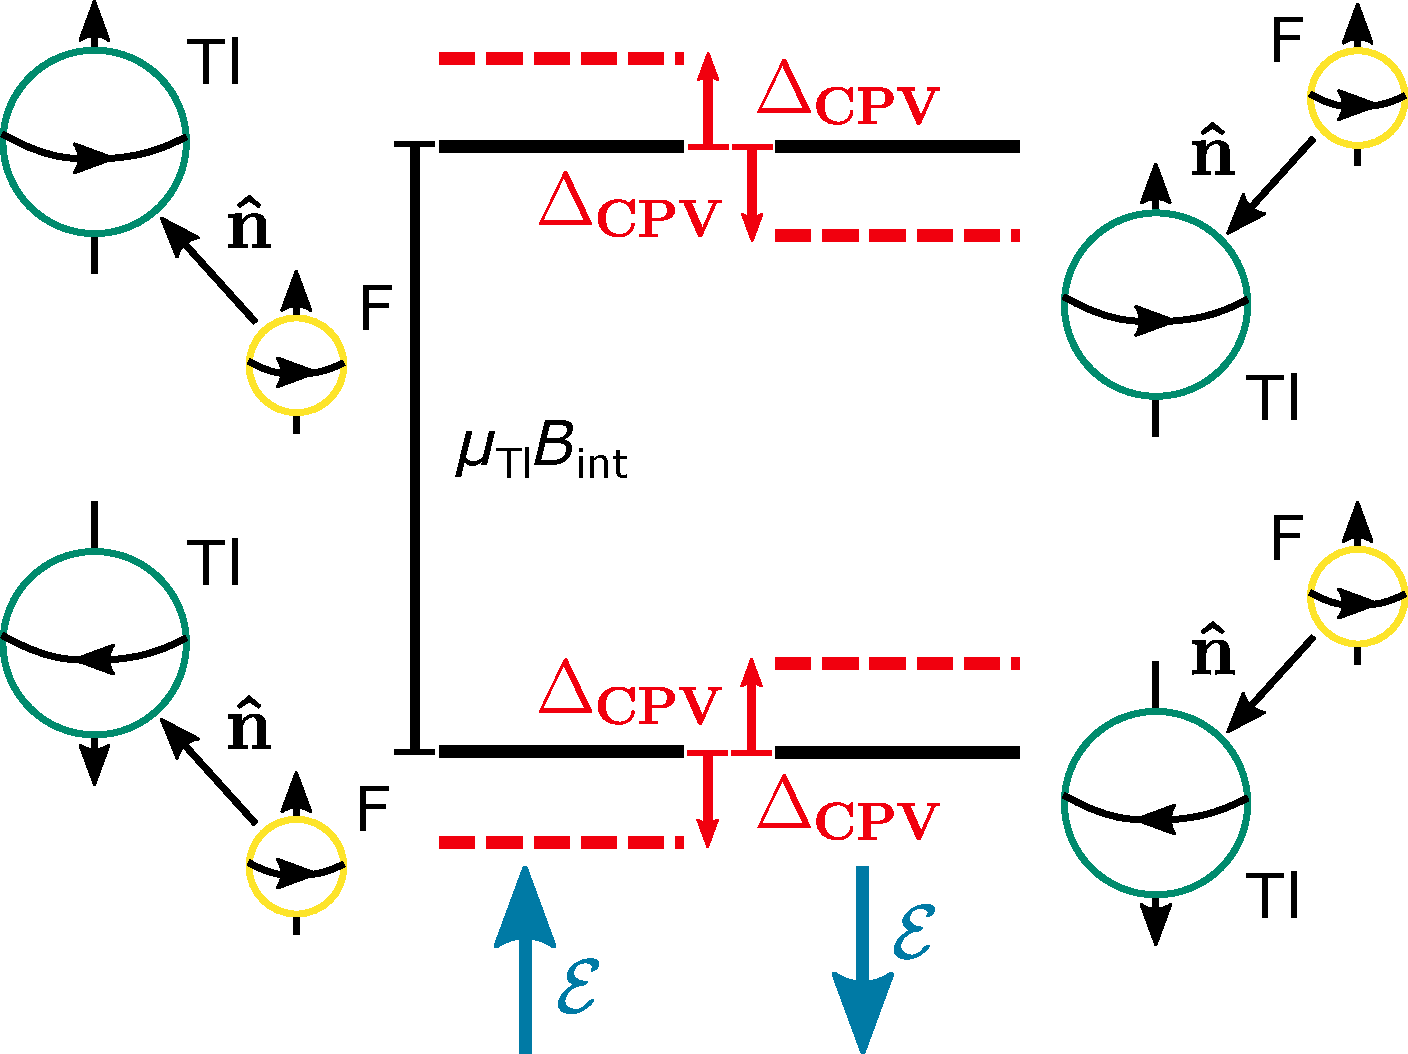
\includegraphics[width=0.48\textwidth,unit=1mm]{figs/svg/edm_levels_pdf_version.pdf}
	\caption{T-violating energy shift $\Delta_{\rm CPV} = W_SS\,\mathcal{P}$ as a result of a nonzero NSM $S$ given by the effective interaction $\mathcal{H}_\text{CPV}= W_S S\vec{I}\cdot \hat{\vec{n}}/I$ (Eq.~\ref{eq:Hamiltonian_effective_interaction}), shown for opposite orientations of the applied field $\Evec$. Here $\mu_1$ is the Tl magnetic moment and $B_1^\mathrm{int}$ is the effective internal magnetic field at the Tl nucleus due to the spin-rotation interaction.
	}
	\label{fig:edm_shift}
\end{figure}

Polar molecules can be polarized readily in laboratory-scale fields owing to their small rotational level separation ($\sim\!10^{-4}\eV$), giving them near-maximal energy shifts induced by a given Schiff moment. Thus, Sandars \cite{sandars1967measurability} suggested a molecular-beam resonance experiment could be used to probe the existence of the proton EDM, if the molecule has a heavy atom with an unpaired proton in the nucleus, such as $^{205}\mathrm{Tl}$. The value of $S$ is determined by measuring energy splittings between spin-up and -down states relative to $\left\langle \hat{\vec{n}}\right\rangle$ (which is parallel to the applied electric field $\bm{\mathcal{E}}$). This splitting will increase or decrease as $\bm{\mathcal{E}}$ (and hence $\left\langle \hat{\vec{n}}\right\rangle$) reverses, due to the interaction in Eq.~\ref{eq:Hamiltonian_effective_interaction}. The difference in level splittings is proportional to the electric polarization $\mathcal{P}$, the interaction strength $W_S$, and $S$ (Fig. \ref{fig:edm_shift}).

\CENTREX\ uses a cold beam of thallium fluoride (TlF) to measure nuclear $T$-violation due to the NSM of the $^{205}$Tl nucleus. It is a suitable system to look for $P$- and $T$-violating interactions for a number of reasons: a molecular beam of thallium fluoride can be readily obtained; many of the molecular states and transitions are known experimentally; the species is a polar diatomic molecule, enhancing the electron density gradient at the site of the nuclei (and hence $W_S$). As the thallium nucleus is heavy $\left(A=205,\,Z=81\right)$ and the NSM-induced energy shift scales $\propto A^{2/3}Z^2$, the observable effect of the Tl Schiff moment is correspondingly large \cite{sandars1967measurability, wilkening1984search}. Since the Tl nucleus contains an unpaired proton,
%the different linear combinations of underlying CPV parameters means
\CENTREX\ will be primarily sensitive to proton EDM effects, as opposed to other leading experiments which are more sensitive to the
%effects associated with neutron spin such as
neutron EDM \cite{graner2016reduced}. TlF is not very sensitive to the electron EDM due to its zero total electron spin \cite{kozlov1995parity}. 

The current best constraint on $T$-violating interactions associated with $S\left(^{205}\mathrm{Tl}\right)$ was found by Cho, Sangster and Hinds in 1991 \cite{cho1989tenfold, cho1991search}, who measured a NSM-induced frequency shift of $\Delta E = 2\Delta_{\rm CPV} = \left(1.4\pm 2.4\right)\times 10^{-4}$~Hz, consistent with zero.\footnote{Throughout, we express both frequencies and energies in linear frequency units (Hz), and all angular momentum operators are treated as dimensionless.} 
Using the effective interaction $\mathcal{H}_\text{CPV}$, the shift in the energy splitting between states with Tl spin up versus spin down, relative to the quantization axis, can be interpreted as
\begin{equation}
    \Delta E= 2 \Delta_{\rm CPV} = 2 W_S\,S\, \textrm{sgn}(\Esca) \,\mathcal{P},
    \label{eq:frequency_shift_due_to_NSM}
\end{equation}
where $W_S = 40539\,$a.u.,
polarization $\mathcal{P} = \langle\hat{\vec{n}} \cdot \hat{\Evec}\rangle = 0.547$, and the sign of $\Esca$ refers to the direction of $\Evec$ relative to a fixed quantizing axis $\hat{z}$.  This determines the Schiff moment \cite{PhysRevA.101.042501, PhysRevLett.88.073001}
\begin{equation}
    S\left(^{205}\mathrm{Tl}\right) = \left(3.6\pm 6.1\right)\times 10^{-11}\,e\,\mathrm{fm}^3.
\end{equation}
With Eq.~\ref{eq:schiff_contributions}, the following limits can be placed:
\begin{equation}
    \label{eq:prev_best_lims}
    \begin{split}
        \bar{\theta} & = \left(1.3 \pm 2.3\right)\ee{-9}, \\
        12\bar{d}_d+9\bar{d}_u & = \left(3.6\pm 6.1\right)\ee{-24}\,\mathrm{cm}, \\
        d_p          & = \left(0.9 \pm 1.5\right)\ee{-23}\,e\,\mathrm{cm},\\
        0.13g\bar{g}_0 - 0.004g\bar{g}_1-0.27g\bar{g}_2 & = \left(3.6 \pm 6.1\right)\ee{-11}.
    \end{split}
\end{equation}
\CENTREX\ aims to improve on these limits by using a cryogenic molecular beam source to achieve a cold beam with higher intensity and lower velocity spread compared to the jet source used in the previous work. Rotational cooling will be performed with optical and microwave pumping, collapsing much of the initial Boltzmann distribution into one state, greatly enhancing the number of molecules accessible for measurement. Finally, optical cycling will be used to assist state readout, resulting in near-unity detection efficiency. Fluorescence detection, compared to the hot-wire techniques used previously, allows for background-free detection if scattered light is well controlled.

\subsection{Thallium Fluoride}
\label{sec:tlf_theory}

\begin{figure}
	    % for axis breaks
    \usetikzlibrary{decorations.markings}
    \def\MarkLt{4pt}
    \def\MarkSep{2pt}
    \tikzset{
      TwoMarks/.style={
        postaction={decorate,
          decoration={
            markings,
            mark=at position #1 with
              {
                  \begin{scope}[xslant=0.2]
                  \draw[line width=\MarkSep,white,-] (0pt,-\MarkLt) -- (0pt,\MarkLt) ;
                  \draw[-] (-0.5*\MarkSep,-\MarkLt) -- (-0.5*\MarkSep,\MarkLt) ;
                  \draw[-] (0.5*\MarkSep,-\MarkLt) -- (0.5*\MarkSep,\MarkLt) ;
                  \end{scope}
              }
           }
        }
      },
      TwoMarks/.default={0.5},
    }

\begin{tikzpicture}[scale=5]

   % length of energy level diagram lines
   \def\len{.05}

   % x-position and length and x-offset of the y-axis labels
   \def\pos{-18}
   \def\lenmark{.025}
   \def\xoffset{.18}

   % x coordinates for m = -2, ... 2
   \def\xa{-4.5*\len}
   \def\xb{-2.5*\len}
   \def\xc{-0.5*\len}
   \def\xd{+1.5*\len}
   \def\xe{+3.5*\len}
   \def\xf{-6.5*\len}
   \def\xg{+5.5*\len}

   % y offset for J = 1, 2
   \def\yA{.6}
   \def\yB{\yA+.7}

   % axis
   \draw[->,TwoMarks=0.2,TwoMarks=0.6] (\xf-\len-\xoffset, -.1)
      -- (\xf-\len-\xoffset,\yB+.25) node[above, xshift = -20] {$E$ [kHz]};

   % brace position
   \def\bracePos{\xg+3*\len}

    
   % J=0 labels
   \draw [decorate,decoration={brace,amplitude=5pt,mirror,raise=4pt},yshift=0pt]
      (\bracePos,-.08) -- node (midJ0) {} (\bracePos,.08) node [black,midway,anchor=west,xshift=25] (nodeJ0) {$0$};
   \draw (\xf-\len-0.5*\lenmark-\xoffset, -.003325) node[anchor=east,below,xshift=\pos]
      {-3.325} -- (\xf-\len+0.5*\lenmark-\xoffset,-.003325) node[right,below,xshift=-\pos] {$1$};
   \draw (\xf-\len-0.5*\lenmark-\xoffset, .009975) node[anchor=east,above,xshift=\pos]
      {9.975} -- (\xf-\len+0.5*\lenmark-\xoffset,.009975) node[right,above,xshift=-\pos] {$0$};

   % J=0 lines
   \draw (\xc, -0.003325) -- (\xc+\len, -0.003325);
   \draw (\xb, -0.003325) -- (\xb+\len, -0.003325);
   \draw (\xd, -0.003325) -- (\xd+\len, -0.003325);
   \draw (\xc, 0.009975) -- (\xc+\len, 0.009975);

   % J=1 labels
   \draw [decorate,decoration={brace,amplitude=10pt,mirror,raise=4pt},yshift=0pt]
      (\bracePos,\yA-.2) -- node (midJ1) {} (\bracePos,\yA+.1) node [black,midway,anchor=west,xshift=25] (nodeJ1) {$1$};
   \draw (\xf-\len-0.5*\lenmark-\xoffset, \yA-.143745) node[anchor=east,below,xshift=\pos] {-143.745} --
      (\xf-\len+0.5*\lenmark-\xoffset,\yA-.143745) node[right,below,xshift=-\pos] {$0$};
   \draw (\xf-\len-0.5*\lenmark-\xoffset, \yA-.121506) node[anchor=east,above,xshift=\pos] {-121.506} --
      (\xf-\len+0.5*\lenmark-\xoffset,\yA-.121506) node[right,above,xshift=-\pos] {$1$};
   \draw (\xf-\len-0.5*\lenmark-\xoffset, \yA+.054446) node[anchor=east,below,xshift=\pos] {54.446} --
      (\xf-\len+0.5*\lenmark-\xoffset,\yA+.054446) node[right,below,xshift=-\pos] {$1$};
   \draw (\xf-\len-0.5*\lenmark-\xoffset, \yA+.068985) node[anchor=east,above,xshift=\pos] {68.985} --
      (\xf-\len+0.5*\lenmark-\xoffset,\yA+.068985) node[right,above,xshift=-\pos] {$2$};

   % J=1 lines
   \draw (\xc, \yA-.143745) -- (\xc+\len, \yA-.143745);
   \draw (\xc, \yA-.121506) -- (\xc+\len, \yA-.121506);
   \draw (\xb, \yA-.121506) -- (\xb+\len, \yA-.121506);
   \draw (\xd, \yA-.121506) -- (\xd+\len, \yA-.121506);
   \draw (\xc, \yA+.054446) -- (\xc+\len, \yA+.054446);
   \draw (\xb, \yA+.054446) -- (\xb+\len, \yA+.054446);
   \draw (\xd, \yA+.054446) -- (\xd+\len, \yA+.054446);
   \draw (\xc, \yA+.068985) -- (\xc+\len, \yA+.068985);
   \draw (\xb, \yA+.068985) -- (\xb+\len, \yA+.068985);
   \draw (\xd, \yA+.068985) -- (\xd+\len, \yA+.068985);
   \draw (\xa, \yA+.068985) -- (\xa+\len, \yA+.068985);
   \draw (\xe, \yA+.068985) -- (\xe+\len, \yA+.068985);

   % J=2 labels
   \draw [decorate,decoration={brace,amplitude=10pt,mirror,raise=4pt},yshift=0pt]
      (\bracePos,\yB-.27) -- node (midJ2) {} (\bracePos,\yB+.18) node [black,midway,anchor=west,xshift=25] (nodeJ2) {$2$};
   \draw (\xf-\len-0.5*\lenmark-\xoffset, \yB-.217455)
   node[anchor=east,left,yshift=-5] {-217.455}
      -- (\xf-\len+0.5*\lenmark-\xoffset,\yB-.217455) node[right,below,xshift=-\pos] {$1$};
   \draw (\xf-\len-0.5*\lenmark-\xoffset, \yB-.172936)
   node[anchor=east,left,yshift=5] {-172.936}
      -- (\xf-\len+0.5*\lenmark-\xoffset,\yB-.172936) node[right,above,xshift=-\pos] {$2$};
   \draw (\xf-\len-0.5*\lenmark-\xoffset, \yB+.105876)
   node[anchor=east,left,yshift=-5] {105.876}
      -- (\xf-\len+0.5*\lenmark-\xoffset,\yB+.105876) node[right,below,xshift=-\pos] {$2$};
   \draw (\xf-\len-0.5*\lenmark-\xoffset, \yB+.141095)
   node[anchor=east,left,yshift=5] {141.095}
      -- (\xf-\len+0.5*\lenmark-\xoffset,\yB+.141095) node[right,above,xshift=-\pos] (J2F3label) {$3$};

   % J=2 lines
   \draw (\xc, \yB-.217455) -- (\xc+\len, \yB-.217455);
   \draw (\xb, \yB-.217455) -- (\xb+\len, \yB-.217455);
   \draw (\xd, \yB-.217455) -- (\xd+\len, \yB-.217455);
   \draw (\xc, \yB-.172936) -- (\xc+\len, \yB-.172936);
   \draw (\xb, \yB-.172936) -- (\xb+\len, \yB-.172936);
   \draw (\xd, \yB-.172936) -- (\xd+\len, \yB-.172936);
   \draw (\xa, \yB-.172936) -- (\xa+\len, \yB-.172936);
   \draw (\xe, \yB-.172936) -- (\xe+\len, \yB-.172936);
   \draw (\xc, \yB+.105876) -- (\xc+\len, \yB+.105876);
   \draw (\xb, \yB+.105876) -- (\xb+\len, \yB+.105876);
   \draw (\xd, \yB+.105876) -- (\xd+\len, \yB+.105876);
   \draw (\xa, \yB+.105876) -- (\xa+\len, \yB+.105876);
   \draw (\xe, \yB+.105876) -- (\xe+\len, \yB+.105876);
   \draw (\xc, \yB+.141095) -- (\xc+\len, \yB+.141095);
   \draw (\xb, \yB+.141095) -- (\xb+\len, \yB+.141095);
   \draw (\xd, \yB+.141095) -- (\xd+\len, \yB+.141095);
   \draw (\xa, \yB+.141095) -- (\xa+\len, \yB+.141095);
   \draw (\xe, \yB+.141095) -- (\xe+\len, \yB+.141095);
   \draw (\xf, \yB+.141095) -- (\xf+\len, \yB+.141095);
   \draw (\xg, \yB+.141095) -- (\xg+\len, \yB+.141095);

   % microwave energies
   \draw[Latex-Latex] (nodeJ0) -- node[above,sloped] {13.3 GHz} (nodeJ1);
   \draw[Latex-Latex] (nodeJ1) -- node[above,sloped] {26.7 GHz} (nodeJ2);

   % approximate F1 labels
   \def\FposX{-5}
   \def\FposY{15}
   \def\FposYY{22}
   \node[xshift=\FposX] at (midJ0) {\nicefrac{1}{2}};
   \node[xshift=\FposX,yshift=-\FposY] at (midJ1) {\nicefrac{1}{2}};
   \node[xshift=\FposX, yshift=\FposY] at (midJ1) {\nicefrac{3}{2}};
   \node[xshift=\FposX,yshift=-\FposYY] at (midJ2) {\nicefrac{3}{2}};
   \node[xshift=\FposX, yshift=\FposYY] at (midJ2) {\nicefrac{5}{2}};
   \node[xshift=\FposX, yshift=47] at (midJ2) (F1label) {$F_1$};
    
   \node at (F1label -| nodeJ2) {$J$};
   \node at (F1label -| J2F3label) {$F$};

\end{tikzpicture}

	\caption{Hyperfine structure in the lowest three rotational levels in the TlF ground state $X^1\Sigma^+$, with no applied fields. Rotational energies $hBJ(J+1)$ should be added to
	%are subtracted from
	the hyperfine energy shifts indicated on the axis. Note the $(2F+1)$-fold degeneracy of each state with total angular momentum $F$, corresponding to the quantum numbers $m_F=-F,\dots,0,\dots,F$.}
	\label{fig:level_diagram}

\end{figure}

The TlF molecule is described by its electronic, vibrational and rotational motion, plus the states of the Tl and F nuclear spins. \CENTREX\ makes use of states both in the vibronic ground state, $X ^1\Sigma^+\left(\nu=0\right)$, and in an electronically excited state, $B ^3\Pi_1\left(\nu=0\right)$.  In both cases, we describe the angular momentum couplings in a Hund's case (a) basis. We typically write energy eigenstates in terms of the basis states $\ket{\eta,J,F_1,F,m_F}$. Here, $\eta$ represents the vibronic quantum numbers; $J$ is the total angular momentum excluding the nuclear spins, $\vec{F}_1 = \vec{J}+\vec{I}_\mathrm{1}$, with $I_\mathrm{1}=1/2$ for $^{205}$Tl; $\vec{F} = \vec{F}_1+\vec{I}_\mathrm{2}$ is the total angular momentum, with $I_\mathrm{2}=1/2$ for $^{19}$F; and $m_F$ is its projection along a quantization axis in the lab frame. Field-free eigenstates are close to these basis states in the ground $X ^1\Sigma^+$ state.  In the $B ^3\Pi_1$ state, strong hyperfine interactions significantly mix states with different $J$ and $F_1$ values. Hence, we describe these eigenstates with the modified notation $\ket{\eta',\widetilde{J}' ,\widetilde{F}_1^\prime,F',m_F'}$, where $\widetilde{J}'$ and $\widetilde{F}_1^\prime$ correspond to the largest component in their basis-state decomposition; the primes indicate that the ket refers to the excited state $B ^3\Pi_1$.

Molecules in the beam are assumed to be in the vibronic ground state, since the beam temperature is much lower than the energy scales associated with the electronic and vibrational excitations. However, even at cryogenic temperatures, there is a Boltzmann distribution over many rotational and nuclear spin states. The dominant term in the energy of rotational/spin levels in the $X ^1\Sigma^+$ state is due to rotation; the mean energy of states with quantum number $J$ is $E_\mathrm{rot}=BJ(J+1)$, where $B\approx 6.67\GHz \approx 0.3\kelvin\,\kB$, where $\kB$ the Boltzmann constant.\footnote{In Ramsey et al.\ \cite{wilkening1984search}, the symbol $B$ denotes the rotational constant in equilibrium position, i.e., there $B\equiv B_\text{e}$. However, the effective $v=0$ rotational constant, $B_0$, is more relevant to \CENTREX. To first order in the Dunham expansion \cite{huber2013molecular}, $B_0=B_\text{e}-\alpha_\text{e}/2$. With $B_\text{e}$ and $\alpha_\text{e}$ from the NIST database \cite{afeefy2011nist}, we find $B_0$. We define the symbol $B\equiv B_0$; its value is shown in Table~\ref{tab:hyperfine_hamiltonian}.}

Hyperfine interactions split sublevels with different $F$ values ($F=J-1,J,J, J+1$, except $F=0,1$ only for $J=0$) in each rotational state. Thus, each rotational level has $4(2J+1)$ magnetic sublevels. %including nuclear spins.
Including rotation, spin-rotation and spin-spin interactions, plus interactions with external electric $(\Evec)$ and magnetic $(\Bvec)$ fields, the system is described by the effective Hamiltonian \cite{wilkening1984search}
\small
$\mathcal{H}_\text{TlF} = \mathcal{H}_\text{rot}+\mathcal{H}_\text{sr}+\mathcal H_\text{ss} + \mathcal H_\text{S}+\mathcal H_\text{Z}$, 
\normalsize
where
\begin{equation} 
    \label{eq:hyperfine_hamiltonian}
    \begin{split}
        \mathcal H_\text{rot} & = B \vec{J}^2 \\
        \mathcal H_\text{sr}&=c_1(\vec I_1\cdot\vec J)+c_2(\vec I_2\cdot\vec J), \\
        \mathcal H_\text{ss}&=c_3 T^2(\vec C)\cdot T^2(\vec I_1, \vec I_2)+c_4(\vec I_1\cdot\vec I_2), \\
        \mathcal H_\text{S}&=-\vec\mu_e\cdot\vec \Evec,\\
        \mathcal H_\text{Z}&=-\frac{\mu_J}{J}(\vec J\cdot\vec \Bvec)-\frac{\mu_1}{I_1}(\vec I_1\cdot\vec \Bvec)-\frac{\mu_2}{I_2}(\vec I_2\cdot\vec \Bvec).
    \end{split}
\end{equation}
Here, the first term in the spin-spin interaction ($\mathcal H_\text{ss}$) contains the scalar product of two rank-2 tensors: one constructed from the modified spherical harmonics $\vec C$, and one from $\vec{I}_1$ and $\vec{I}_2$ \cite{brown2003rotational}. (The matrix elements diagonal in $J$ of this term are given in \cite{wilkening1984search}.)  The hyperfine parameters $c_1,c_2,c_3,c_4$, rotational constant $B$, magnetic moments $\mu_J,\mu_1,\mu_2$, and molecule-frame electric dipole moment $\mu_e$ are all known from previous measurements; their values are given in  Table~\ref{tab:hyperfine_hamiltonian}. A level diagram of low-lying states in the absence of applied fields is shown in Fig.~\ref{fig:level_diagram}.

\begin{table}
    \small
    \setlength\extrarowheight{3pt}
    \rowcolors{2}{white}{gray!25}
	\centering
	\caption{Constants describing rotational, hyperfine, Zeeman, and Stark interactions in the effective TlF ground-state  Hamiltonian (Eq.~\ref{eq:hyperfine_hamiltonian}). All values taken from Ramsey et al.\ \cite{wilkening1984search}, except for $B$ (see Sec. \ref{sec:tlf_theory}).}
	\label{tab:hyperfine_hamiltonian}
	\begin{tabular}{r@{\hspace{5pt}}c@{\hspace{5pt}}l@{\hspace{5pt}}l | r@{\hspace{5pt}}c@{\hspace{5pt}}l@{\hspace{5pt}}l}
    	\toprule
		$B$ & = &           $6.66733$ &     GHz &       $\mu_e$ & = & $4.2282(8)$ &     Debye \\
		$\mu_J$ & = &       $35(15)$ &      Hz/G &      $c_1$ & = & $126.03(12)$ &    kHz \\
		$\mu_1^{205}$ & = & $1.2405(3)$ &   kHz/G &     $c_2$ & = & $17.89(15)$ &     kHz\\
		$\mu_1^{203}$ & = &  $1.2285(3)$ &   kHz/G &     $c_3$ & = & $0.70(3)$ &       kHz \\
		$\mu_2$ & = &      $2.00363(4)$ &  kHz/G  &    $c_4$ & = & $-13.30(72)$ &    kHz \\
		\bottomrule
	\end{tabular}
\end{table}

%%%%%%%%%%%%%%%%%%%%%%%%%%%%%%%%%%%%%%%%%%%%%%55%%%%%%%%%%%%%%%
In \CENTREX, lasers are tuned to $X^1\Sigma^+(\nu=0)\rightarrow B^3\Pi_1\left(\nu=0\right)$ transitions in order to manipulate and read out ground state hyperfine and rotational sublevels. Details of the $B ^3\Pi_1$ state structure are given in \cite{norrgard2017hyperfine,PhysRevA.101.042506}.  Here, only a few main features of the $B$ state substructure are important.  First, the $B$ state hyperfine splittings are very large ($\gtrsim 100\MHz$) compared to the natural linewidth of the transition ($\gamma_B \approx 1.6\MHz$), which is in turn much larger than the ground-state hyperfine splittings ($c_j \lesssim 100\kHz$). This means that hyperfine structure is fully resolved in the excited state, and entirely unresolved in the ground state. Hence, optical transitions in TlF drive a large manifold of ground-state hyperfine levels (with a given value of $J$) to a single hyperfine state with (nominal) quantum numbers $\tilde{J},\tilde{F}_1$ and exact quantum number $F$. Another important feature of the $B$ state is that its matrix of Franck-Condon factors (FCFs) for decay to the $X$ state is extremely diagonal \cite{hunter2012prospects}, such that $\sim\! 99\%$ of the time, the $B(v=0)$ vibronic state decays back to the vibronic ground state $X(v=0)$.  This enables optical pumping and optical cycling with little loss.  However, the mixing of $J$ and $F_1$ by the strong $B$-state hyperfine interaction substantially modifies rotational selection rules in $B-X$ decays, and must be taken into account when describing optical excitation and emission in TlF.

\subsection{TlF in \texorpdfstring{$\Esca$}{E}-fields}
\label{sec:TlF_in_E_fields}

\begin{figure*}
	\centering
	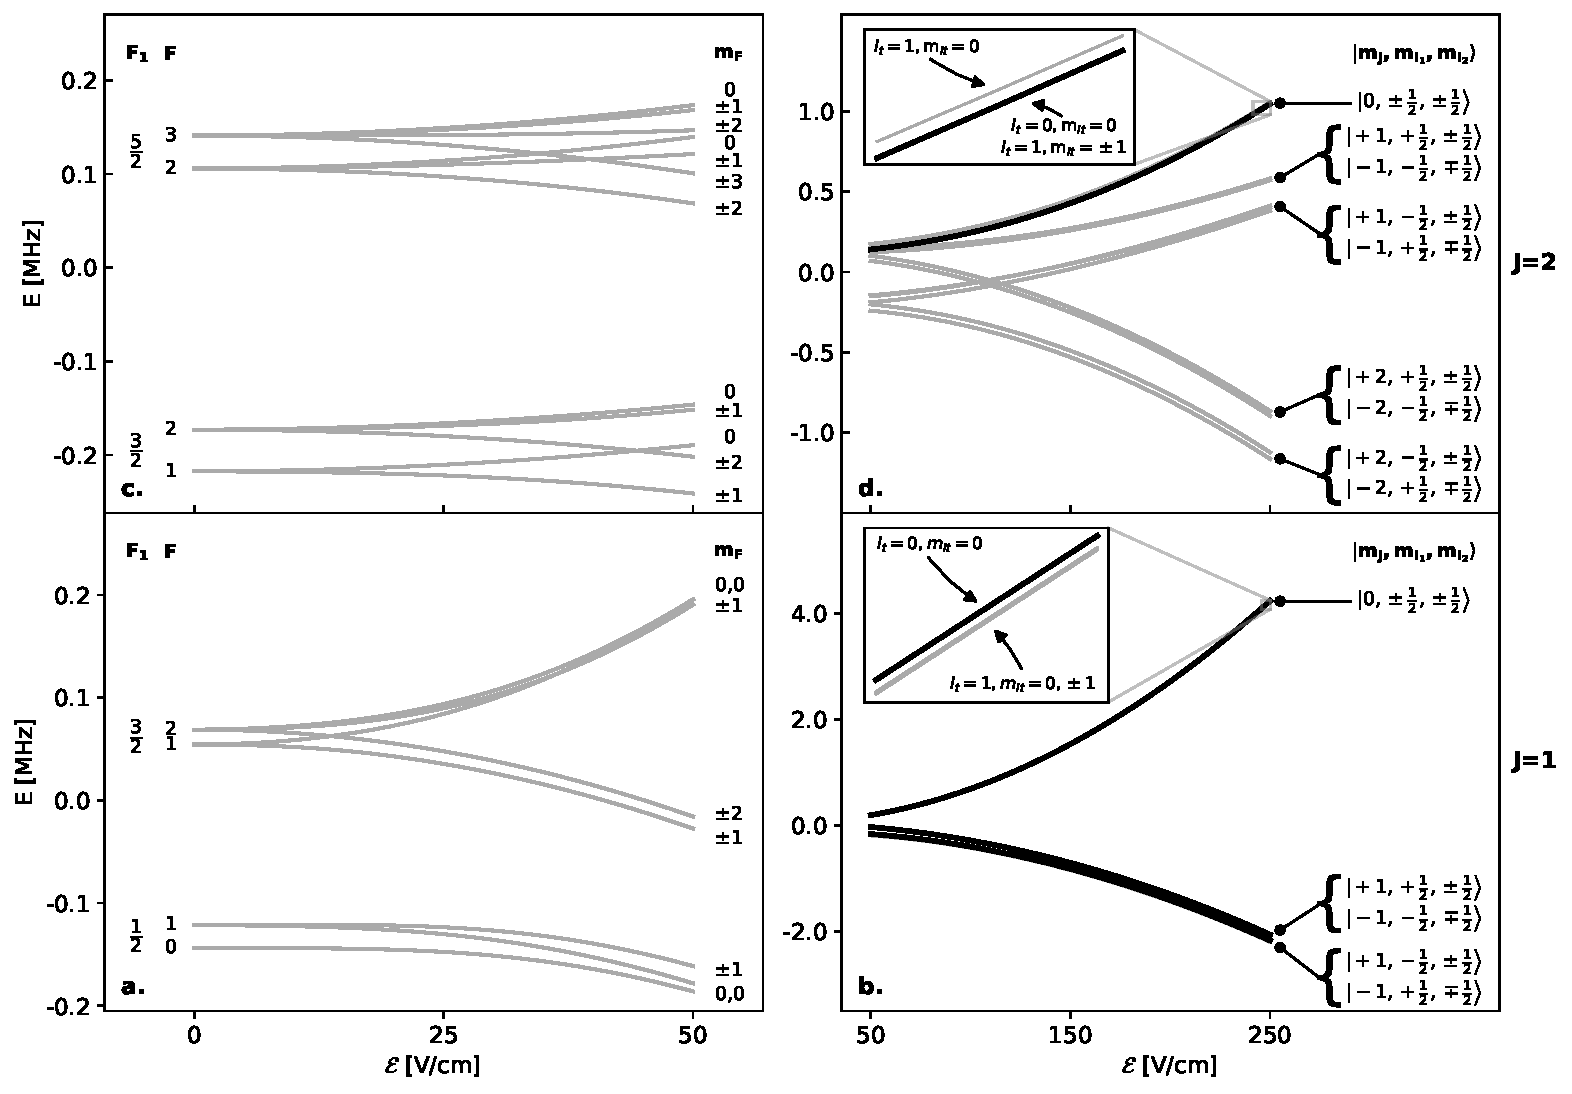
\includegraphics[width=\textwidth]{figs/matplotlib/low_to_mid_field.pdf}
	\caption{Overview of the energy eigenstates for changing $\Esca$-field magnitudes. The low-field regime, where $\Delta E_{\rm S} \ll E_{\rm hf}$, where energy eigenstates retain $J$, $F$, and $F_1$ as approximate quantum numbers is shown in \part{a} for $J=1$ and \part{c} for $J=2$. The mid-field regime, where $E_{\rm hf} \ll \Delta E_{\rm S} \ll E_{\rm rot}$, where both $J$ and $m_J$ are approximate quantum numbers is shown in \part{b} for $J=1$ and \part{d} for $J=2$. States used in \CENTREX\ are shown in bold.}
	\label{fig:low_to_mid_field}
\end{figure*}

\begin{figure}
	\centering
	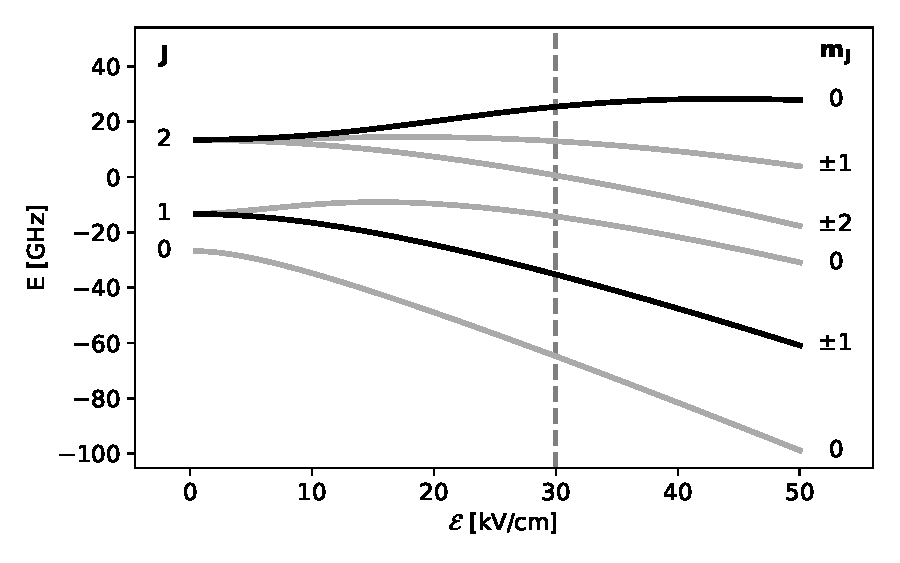
\includegraphics[width=\textwidth/2]{figs/matplotlib/low_to_high_field.pdf}
	\caption{Evolution of the energy eigenstates of the TlF Hamiltonian (Eq. \ref{eq:hyperfine_hamiltonian}) for $\Esca$ ranging from $0\,$V/cm to $50\,$kV/cm, for $J=0,1,2$. States used in \CENTREX\ are shown in bold. Hyperfine structure is unresolved in this plot.}
	\label{fig:low_to_high_field}
\end{figure}

Throughout most of the \CENTREX\ apparatus, TlF molecules experience a non-zero $\Esca$-field and (nominally) zero $\Bsca$-field.
The character of the energy eigenstates changes significantly depending on the $\Esca$-field magnitude, which varies dramatically between stages of the experiment. Hence, it is useful to describe the energy eigenstates of the TlF electronic ground state in different regimes of $\Esca$-field strength (with $\Bsca = 0$), as defined by the ratio of Stark shifts, $\Delta E_{\rm S} = \langle \mathcal{H}_{\rm S}\rangle \sim \mu_e^2 \Esca^2/B$, to the strength of hyperfine interactions, $E_{\rm hf} = \langle \mathcal{H}_{\rm sr} + \mathcal{H}_{\rm ss}\rangle \sim c_j$, or rotational energies, $E_{\rm rot} = \langle \mathcal{H}_{\rm rot}\rangle \sim B$. In all regimes, the total angular momentum projection $m_F$ along 
a space-fixed quantization axis $\hat{z}$ (always defined such that $\Evec$ is very nearly parallel to $\hat{z}$), is an exact quantum number.

In the low-field regime, where $\Delta E_{\rm S} \ll E_{\rm hf}$, energy eigenstates retain $J$, $F$, and $F_1$ as approximate quantum numbers. 
In the mid-field regime, where $E_{\rm hf} \ll \Delta E_{\rm S} \ll E_{\rm rot}$, both $J$ and $m_J$ are approximate quantum numbers. 
Here, the tensor part of the Stark shifts gives rise to energy splittings between levels with different values of $|m_J|$ that are comparable in size to the scalar shifts, i.e., of order $\Delta E_{\rm S}$.  Thus, when $m_J\neq 0$, $\vec{J}$ is strongly coupled to $\Evec$ (and hence to the molecular axis $\vec{\hat{n}}$) by this Stark interaction. In this case, each nuclear spin is coupled to $\vec{J}$ (and thus also to $\Evec$) by the spin-rotation interactions of $\mathcal{H}_{\rm sr}$. Hence, here $m_{I_1}$ and $m_{I_2}$ are approximate quantum numbers. By contrast, in states where $m_J=0$ (including when $J=0$) in this regime, $\left\langle \mathcal{H}_{\rm sr}\right\rangle$ vanishes to first order, and the nuclear spins do not couple to $\vec{J}$ and $\Evec$. However, the nuclear spins remain coupled to each other via the spin-spin interaction $\mathcal{H}_{\rm ss}$.  So, here the total nuclear spin $\vec \It = \vec I_1 + \vec I_2$ and its projection $m_{\It}$ are approximate quantum numbers in addition to $J$ and $m_J=0$. 
Finally, in the high-field regime where $E_{\rm hf} \ll E_{\rm rot} \lesssim \Delta E_{\rm S}$, $J$ states are strongly mixed, and separations between $m_J$ states are on the order of $E_{\rm rot}$. Here, eigenstates are defined by the same approximate quantum numbers as in the mid-field regime, aside from $J$. We refer to these strongly mixed states with the label $\widetilde{J}$, which corresponds to the value of $J$ that any given state connects to adiabatically, if the $\Esca$-field is reduced.
Table \ref{tab:E_field_regimes} summarizes the different regimes and associated eigenstates.  
\begin{table*}[t]
    \centering
    \def\colseplarge{4ex} % should only be used in this table
	\begin{tabular}{@{}r@{\hspace{\colseplarge}}r@{$\,\Delta E_{\rm S}\,$}l@{\hspace{\colseplarge}}r@{$\,\Esca\,$}l@{\hspace{\colseplarge}}>{\raggedright\arraybackslash}m{4cm}@{}}
    	\toprule
    	Regime & \multicolumn{2}{c}{Definition} & \multicolumn{2}{c}{Field strength} & Approx. eigenstates \\
		\midrule
		 Low
		 & & $\ll E_{\rm hf}$
		 & & $\lesssim 50 \Vcm$
		 & $\ket{J,F_1,F,m_F}$ \\\addlinespace[2ex]
		 %
	     Mid
	     & $E_{\rm hf} \ll$ & $\ll E_{\rm rot}$
	     & $50 \Vcm \ll$ & $\lesssim 5 \kVcm$
	     & $\ket{J,m_J \neq 0}\ket{m_{I_1},m_{I_2}}$ 
	       $\ket{J,m_J=0}\ket{\It,m_{\It}}$ \\\addlinespace[2ex]
	     %
	     High
	     & $E_{\rm hf} \ll E_{\rm rot} \lesssim$ &
	     & $5\kVcm \ll$ &
	     & $\ket{\widetilde{J},m_J\neq 0} \ket{m_{I_1},m_{I_2}}$
	       $\ket{\widetilde{J},m_J=0}\ket{\It,m_{\It}}$ \\
		\bottomrule
	\end{tabular}
	\caption{Regimes of electric field strength and associated eigenstates in TlF.}
	\label{tab:E_field_regimes}
\end{table*}


Figure \ref{fig:low_to_mid_field} shows how the relevant energies and eigenstates evolve from the low-field to the mid-field regime for $J=1$ and $J=2$ states.  Bold curves are states directly relevant to \CENTREX. Figure \ref{fig:low_to_high_field} shows a zoom out of states up to $J=2$ from low to high fields.

The $^{205}$Tl NSM measurement is carried out in $\tilde{J} = 1,\, m_J = \pm1$ states of TlF at large electric field $\mathcal{E} = 30$ kV/cm. This choice of states takes advantage of the structure of TlF in electric fields, in two ways. First, the observable energy shift associated with $S$, $\Delta E$, scales linearly with the degree of polarization $\mathcal{P}$ of the TlF molecule (Eq. \ref{eq:frequency_shift_due_to_NSM}). An electric field more easily polarizes states with low $J$, since $\mathcal{P}$ arises from mixing between states with different parity and thus different $J$; these states are closest together when $J$ is small. Additionally, as discussed in Sec. \ref{Sec:InternalComagnetometry}, certain dangerous systematic errors in the NSM measurement are dramatically suppressed in the presence of a strong spin-rotation interaction (later referred to as an effective intra-molecular magnetic field). This requires $m_J \neq 0$. The $\tilde{J} = 1,\, m_J = \pm1$ states hence provide the best combination of sensitivity and systematic error suppression in TlF.\footnote{$|\mathcal{P}|$ is larger in the $J=0,m_J = 0$ states, given the same $\Esca$-field value. Hence, the NSM gives larger energy shifts there. However, in these states where $m_J = 0$, the effective intra-molecular magnetic field vanishes.}

\section{Methods}
\label{sec:methods}

% \begin{figure*}
% % \begin{minipage}{\textwidth}
%   \centering
%   \begin{minipage}{.45\textwidth}
%      \centering
%         % \begin{algorithm}
%         % \caption{Extending episodic learning to multiple tasks in the training corpus. SAMPLE$(S,K)$ denotes selecting $K$ samples uniformly at random from set $S$ with replacement.}
%         % \label{algo:ProtoNet}
%         \hspace*{\algorithmicindent} \textbf{Input:} T: set of tasks, N: number of episodes
%         \begin{algorithmic}[1]
%         \For{i $\in \{1...N\}$}
%             \State $t \gets $SAMPLE$(T,1)$. \Comment{Sample a task}
%             \For{c in $\{1...C\}$}
%                 \State $D_{t,c} \gets$ Embeddings $\in$ class $c$ in task $t$
%                 \State $S_{t,c} \gets $SAMPLE$(D_{t,c},k)$ \Comment{k supports}
%                 \State $Q_{t,c} \gets $SAMPLE$(D_{t,c},q)$ \Comment{q queries}
%             \EndFor
%             \State Perform Episodic Training: Equations (\ref{eqn:proto_basic}-\ref{eqn:proto_backprop})
%         \EndFor
%         \end{algorithmic}
%         % \end{algorithm}
%   \end{minipage}
%   \begin{minipage}{.45\textwidth}
%      \centering
%         % \begin{algorithm}
%         % \caption{Extending episodic learning to multiple tasks in the training corpus. SAMPLE$(S,K)$ denotes selecting $K$ samples uniformly at random from set $S$ with replacement.}
%         % \label{algo:ProtoNet}
%         \hspace*{\algorithmicindent} \textbf{Input:} T: set of tasks, N: number of episodes
%         \begin{algorithmic}[1]
%         \For{i $\in \{1...N\}$}
%             \State $t \gets $SAMPLE$(T,1)$. \Comment{Sample a task}
%             \For{c in $\{1...C\}$}
%                 \State $D_{t,c} \gets$ Embeddings $\in$ class $c$ in task $t$
%                 \State $S_{t,c} \gets $SAMPLE$(D_{t,c},k)$ \Comment{k supports}
%                 \State $Q_{t,c} \gets $SAMPLE$(D_{t,c},q)$ \Comment{q queries}
%             \EndFor
%             \State Perform Episodic Training: Equations (\ref{eqn:proto_basic}-\ref{eqn:proto_backprop})
%         \EndFor
%         \end{algorithmic}
%         % \end{algorithm}
%   \end{minipage}
%   \caption{figure}{Two algorithms side by side}
%   \label{fig:twoalg}
% % \end{minipage}
% \end{figure*}

In this section, we introduce the meta-learning setup for neural embedding training followed by description of two metric-learning approaches adopted in this work: prototypical networks and relation networks. Following which, we outline their use in our tasks: speaker diarization and speaker verification, including a description of the choice of clustering algorithm.

Consider a training corpus where $C$ denotes the set of unique speakers, and where each speaker has multiple utterances available. Typically, $|C|$ is a large integer
($\mathcal{O}(10^3)$).  
Here, an utterance might be in the form of raw waveform or frame-level features such as MFCCs or Mel spectrogram. 
%During conventional classification, a minibatch is randomly sampled from the training corpus wherein both the speakers and number of samples per speaker are simultaenously sampled. The final layer in a DNN is fixed-dimensional, i.e $N$. 
Under the meta-learning setup, each episode (a training step; equivalent to a minibatch) consists of two stages of sampling: classes and utterances conditioned on classes. 
First, a subset of classes $L$ (speakers) is sampled from $C$ within an episode, with the number of speakers per episode $|L|$ typically held constant during the training process. 
Next, two disjoint sets from each speaker in $L$ are sampled without replacement from the set of all utterances belonging to that speaker: supports $S$ and queries $Q$. 
Within an episode, supports and queries are used for model training and loss computation, respectively, similar to train and test sets in supervised training. This process continues across a large number of episodes with speakers and utterances sampled as explained above.
Following terminology from Section \ref{sec:intro}, an episode is equivalent to a \textit{task}, wherein the model learns to classify speakers from that task. Hence, meta-learning optimizes across tasks, treating each task as a training example. The optimization process is given as:
\begin{equation}
    \theta = \argmax_{\theta} \displaystyle \mathop{\mathbb{E}}_{L} [ \mathop{\mathbb{E}}_{S, Q} [ \mathop{\mathbb{E}}_{(\mathbf{x},y) \in Q} [ \log p_\theta (y|\mathbf{x},S)] ]]
\end{equation}
% \begin{equation}
%     \theta = \argmax_{\theta} \displaystyle \mathop{\mathbb{E}}_{L \sim C} [ \mathop{\mathbb{E}}_{\substack{S \sim L\\ Q \sim L}} [ \mathop{\mathbb{E}}_{(x,y) \in Q} \log p_\theta (y|x,S) ]]
% \end{equation}
Here, $\theta$ denotes trainable parameters of the neural network, $(\mathbf{x},y)$ represents an utterance and its corresponding speaker label. In contrast to conventional supervised learning:
\begin{equation}
    \theta = \argmax_{\theta} \displaystyle \mathop{\mathbb{E}}_{B} [  \mathop{\mathbb{E}}_{(\mathbf{x},y) \in B}[\log p_\theta (y|\mathbf{x})]  ]
\end{equation}
where $B$ denotes a minibatch. Meta-learning approaches are broadly categorized based on the characterization of $p_\theta (y|x)$: model-based \cite{santoro2016meta}, metric-based \cite{vinyals2016matching} and optimization-based meta-learning \cite{finn_maml2017}. 
Of interest in this work are metric-based approaches where $p_\theta (y|x)$ is a potentially learnable kernel function between utterances from $S$ and $Q$. The reasoning is as follows: speaker embeddings trained for classification are bottleneck representations, and the latter is directly optimized using task performance in metric-learning approaches. We now describe the two metric-learning approaches used in this work: prototypical networks and relation networks.

\subsection{Prototypical Networks}

Protonets learn a non-linear transformation where each class is represented by a single point in the embedding space, namely the centroid (prototype) of training utterances from that class. During inference a test sample is assigned to the class of nearest centroid, similar to the nearest class mean method \cite{mensink2013}. 

At training time, consider an episode $t$, the support set ($S_t$) and the query set ($Q_t$) sampled as explained above. Supports are used for prototype computation while queries are used for estimating class posteriors and loss value. 
%Protonets learn the mapping $f_{\theta} : \mathbb{R}^M \rightarrow \mathbb{R}^P$ where the prototype of each class is computed as follows:
The prototype ($\mathbf{v}_c$) for each class is computed as follows:
\begin{equation}
\label{eqn:proto_basic}
    \mathbf{v}_{c} = \frac{1}{|S_{t,c}|} \sum_{(\mathbf{x_{i}},y_{i})\in S_{t,c}} f_{\theta}(\mathbf{x}_i)
\end{equation}
$f_{\theta} : \mathbb{R}^M \rightarrow \mathbb{R}^P$ represents the parameters of the protonet. $\mathbf{x_i}$ represents an $M$-dimensional utterance representation extracted using a DNN.
$S_{t,c}$ is the set of all utterances in $S_t$ belonging to class $c$. For every test utterance $\mathbf{x_j} \in Q_t$, the posterior probability is computed by applying softmax activation over the negative distances with prototypes:
\begin{equation}
\label{sofmax-eq2}
    p_\theta(y_j=c\,| \mathbf{x}_j, S_t)=\frac{\exp \left(-d\left(f_{\theta}(\mathbf{x}_j), \mathbf{v}_c\right)\right)}{\sum_{c^{\prime} \in L} \exp \left(-d\left(f_{\theta}(\mathbf{x}_j), \mathbf{v}_{c^{\prime}}\right)\right)}
\end{equation}
$d$ represents the distance function. 
Squared Euclidean distance was proposed in the original formulation \cite{snell2017prototypical} due to its interpretability as 
a Bregman divergence \cite{banerjee2005} as well as supporting empirical results. For the above reasons, we adopt squared Euclidean as a metric in this work.
The negative log-posterior is treated as the episodic loss function and minimized using gradient descent:
\begin{equation}
\label{eqn:proto_backprop}
 \text{Loss} = - \frac{1}{|Q_t|} \sum_{(\mathbf{x}_j,y_{j})\epsilon Q_t } \log(p_\theta(y_j \mid \mathbf{x}_j, S_t)) 
\end{equation}

\subsection{Relation Networks}

Relation networks compare supports and queries by learning the kernel function simultaneously with the embedding space\cite{sung2018learning}. In contrast with protonets which use squared Euclidean distance, relation networks learn a more complex inductive bias by parameterizing the comparison metric using a neural network. 
Hence, relation networks attempt to jointly learn the embedding and metric over an ensemble of tasks that are generalized to an unseen task. Specifically, there exist two modules: an encoder network that maps utterances into fixed-dimensional embeddings and a comparison network that computes a scalar relation given pairs of embeddings. Given supports $S_t$ within an episode $t$, the class representation is taken as the sum of all support embeddings:
\begin{equation}
\label{eqn:relation_encoder}
    \mathbf{v}_c = \sum_{(\mathbf{x}_i,y_{i})\epsilon S_{t,c}} f_{\theta}(\mathbf{x}_i)
\end{equation}
$f_{\theta}$ represents the encoder network. For each query embedding belonging to a class $j$, its relation score $r_{c,j}$ with training class $c$ is computed using the comparison network $g_{\phi}$ as follows:
\begin{equation}
\label{eqn:relation_relation}
    r_{c,j} = g_{\phi} ([ \mathbf{v}_c, f_{\theta} (\mathbf{x}_j) ])
\end{equation}
Here $[.,.]$ represents concatenation operation. The original formulation of relation networks \cite{sung2018learning} treated the relation score as a similarity measure, hence $r_{c,j}$ is trained with:

\begin{equation}
    r_{c,j}= 
\begin{cases}
    1, & \text{if } y_j = c\\
    0, & \text{otherwise}
\end{cases}
\end{equation}

In the original formulation \cite{sung2018learning}, the networks $f_\theta$ and $g_\phi$ were jointly optimized using mean squared error (MSE) objective since the predicted relation network was treated similar to a linear regression model output. In this work, we replace MSE with the conventional cross-entropy objective based on empirical results. Hence the posterior probability is computed as:
\begin{equation}
\label{softmax-eq}
    p_\theta(y_j| \mathbf{x_j}, S_t)=\frac{\exp \left(  r_{c,j}   \right)}{\sum_{c^{\prime} \in L} \exp \left(    r_{c^{\prime},j}     \right)}
\end{equation}
and the loss function is computed using Eq. \ref{eqn:proto_backprop}.

\subsection{Use in Speaker Applications}

\subsubsection{Speaker Diarization}
\label{subsubsec:bSCNME}
Typically, there exist four steps in a speaker diarization system: speech activity detection, speaker segmentation, embedding extraction and speaker clustering (exceptions include recently proposed end-to-end approaches \cite{horiguchi2020endtoend,fujita2020endtoend}). In this work, we adopt the uniform segmentation strategy similar to \cite{Sell2018_dihard, garciaRomero2017} wherein the session is segmented into equal duration segments with overlap. Meta-learned embeddings are extracted from these segments followed by clustering. We use a recently proposed variant of spectral clustering \cite{park_SC2020} which uses a binarized version of affinity matrix between speaker embeddings. The binarization is expressed using a parameter ($p$) which represents the fraction of non-zero values at every row in the affinity matrix.
The clustering algorithm attempts a tradeoff between pruning excessive connections in the affinity matrix (minimizing $p$) while increasing the normalized maximum eigengap (NME; $g_p$) where the latter is expressed as a function of $p$ (Eq. (10) in \cite{park_SC2020}). The ratio ($\frac{p}{g_p}$) is then minimized to estimate the number of resulting clusters (i.e., speakers) in a session. This process is referred to as binarized spectral clustering with normalized maximum eigengap (NME-SC).

Our choice of NME-SC in this work is motivated by two reasons: (1) We do not require a separate development set to estimate a threshold parameter used in the more common agglomerative hierarchical clustering (AHC) method with average linking applied on distances estimated using probabilistic linear discriminant analysis (PLDA) \cite{Sell2018_dihard}. We choose the binarization parameter ($p$) for each session by optimizing for ($\frac{p}{g_p}$) over a pre-determined range for $p$. (2) Empirical results which demonstrate similar performance between AHC tuned on a development set and NME-SC reported in \cite{park_SC2020} and in this work. 

\subsubsection{Speaker Verification}
We use the standard protocol for speaker verification wherein a speaker embedding is extracted from the entire utterance. Subsequently, the embeddings are reduced in dimension using LDA and trial pairs are scored using a PLDA model trained on the same data used to train embeddings. Following this, target/imposter pairs are determined using a threshold on the PLDA scores.

\begin{figure*}
    \centering
    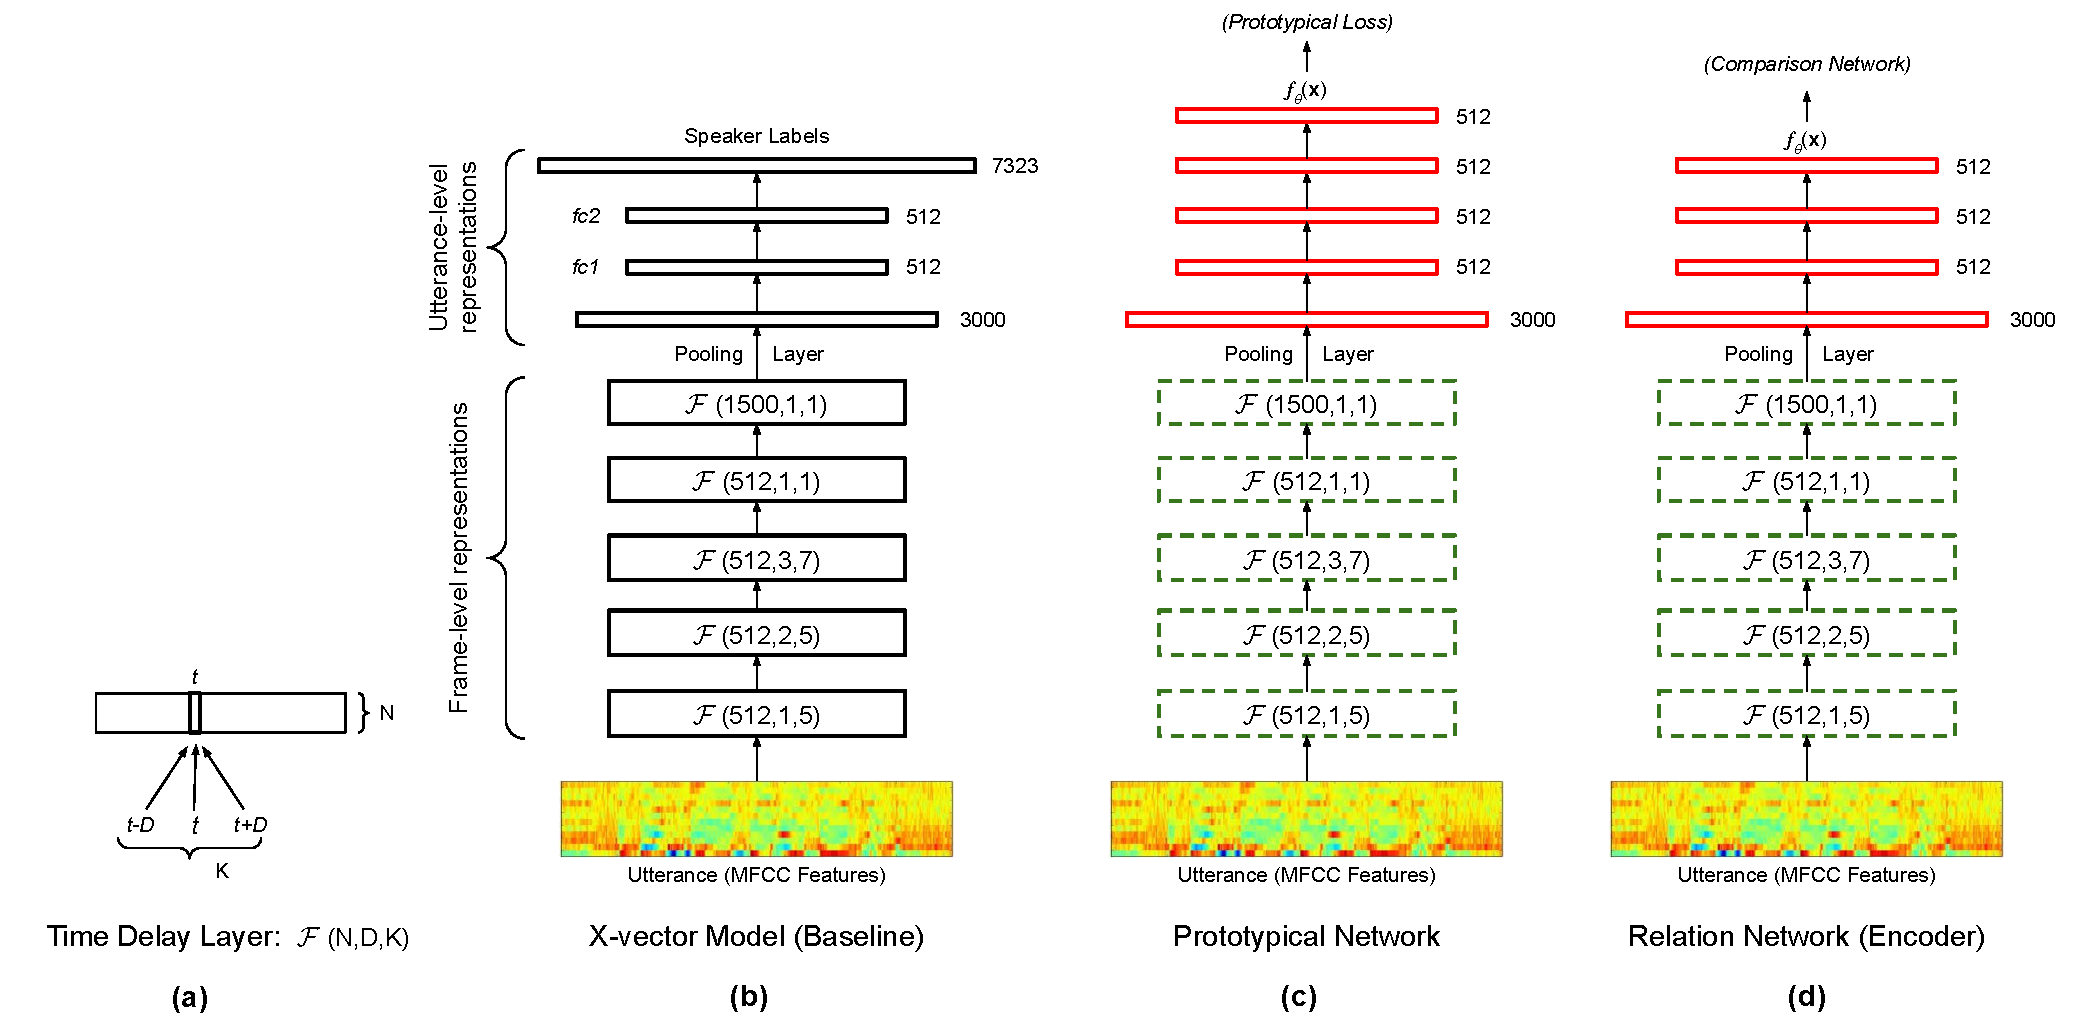
\includegraphics[width=\textwidth]{fig/meta_learning_arch.pdf}
    \caption{Overview of baseline and meta-learning architectures. \textbf{(a)} A time-delay layer $\mathcal{F}(N,D,K)$ which forms the basic component across models. At each time-step, activations from the previous layer are computed using a context width of $K$ and a dilation of $D$. $N$ represents the output embedding dimension. \textbf{(b)} Baseline x-vector model. Kaldi speaker embeddings are extracted at fc1 layer. We find that fc2 and fc1 embeddings perform better for speaker diarization and speaker verification respectively. \textbf{(c)} Prototypical network architecture. Layers marked with a dashed boundary are initialized with pre-trained x-vector models, while layers with a solid boundary are randomly initialized. The final layer output is referred to as protonet embeddings. \textbf{(d)} Relation encoder architecture. The final layer output is referred to as relation network embeddings. Relation scores are computed used these embeddings as illustrated in Fig. \ref{fig:metaLearningLoss}b) }
    \label{fig:metaLearningArch}
\end{figure*}


% Talk about the evaluation methods for each application
% % Speaker Diar
% We use DER, which is .....
% We do not use any collar, like the recent DIHARD. However, we do remove overlapping regions since neither baseline nor proposed systems take it into account
% We assume VAD is available in all our experiments 

% % SV
% We use EER, which is

\paragraph{Sampling CF data.} Sampling in CF-data has been a popular choice for three major scenarios. Most prominently, sampling is used for mining hard-negatives while training recommendation algorithms. Some popular approaches include random sampling; using the graph-structure % to find the hardest negatives 
\cite{pinsage, eclare}; and ad-hoc techniques like similarity search \cite{slice}, stratified sampling \cite{sampling_cf_nn}, \etc % On the other hand, 
Sampling is also generally employed for evaluating recommendation algorithms by estimating expensive to compute metrics like Recall, nDCG, \etc \cite{sampled_metrics, castells_sampling}. Finally, sampling is also used to create smaller sub-samples of 
% the \emph{entire} data 
a big dataset
for reasons like fast experimentation, benchmarking different algorithms, privacy concerns, \etc However, the consequences of different samplers on any of these downstream applications is under-studied, and is the main research interest of this paper. 

\paragraph{Coreset selection.} Closest to our work, a coreset is loosely defined as a subset of data-points that maintains a similar ``quality'' as the full dataset for subsequent model training. Submodular approaches try to optimize a function $f : \mathbf{V} \mapsto \mathcal{R}_+$ which measures the utility of a subset $\mathbf{V} \subseteq \mathbf{X}$, and use it as a proxy to select the best coreset \cite{coreset_1}. More recent works treat coreset selection as a bi-level optimization problem \cite{coreset_bilevel, coreset_bilevel_2} and directly optimize for the best coreset for a given downstream task. Selection-via-proxy \cite{svp} is another technique which employs a base-model as a proxy to tag the importance of each data-point. Note, however, that 
% all of the discussed 
most existing
coreset selection approaches were designed primarily for classification data, whereas adapting them for CF-data is non-trivial because of: (1) the inherent data heterogeneity; the (2) wide range of recommendation metrics; and (3) the prevalent missing-data characteristics.

\paragraph{Evaluating sample quality.} The quality of a dataset sample, if estimated correctly is of high interest for various applications. Short of being able to evaluate the ``true'' utility of a sample, one generally resorts to either retaining task-dependent characteristics \cite{evaluate_sample_quality_1} \emph{or} employing universal, handcrafted features like a social network's hop distribution, eigenvalue distribution, \etc \cite{large_graphs} as meaningful proxies. Note that evaluating the sample quality with a limited set of handcrafted features might introduce bias in the sampled data, depending on the number and quality of such features.


\section{Experiments}
We conduct experiments on two ultra-fine entity typing datasets, {\bf \textsc{UFET}} (English) and {\bf \textsc{CFET}} (Chinese). Their data statistics are shown in Table \ref{tab:stat}. We mainly focus on and report the macro-averaged recall at the recall and expand stage, and concern mainly on the macro-$F1$ of the final prediction at the filter stage. We also evaluate the {\bf \textsc{\name}} models on the fine-grained (130 types) and coarse-grained (9 types) settings of entity typing without the recall and expand stage.
\subsection{UFET and CFET}
\subsubsection{Recall Stage}
\label{sec:recall}
We compare the recall@$K$ on the test sets of {\bf \textsc{UFET}} and {\bf\textsc{CFET}} between the trained MLC model (introduced in \ref{sec:mlc}) and a traditional BM25 model \cite{bm25} in Figure \ref{fig:recall}. The MLC model uses the RoBERTa-large as backbone and is tuned based on the recall@$128$ on the development set. We use AdamW optimizer with a learning rate of $2\times10^{-5}$. Results show that MLC is a strong recall model, it consistently has better recall compared to BM25 on both {\bf\textsc{UFET}} and {\bf\textsc{CFET}} dataset, and the recall@$128$ reaches over $85\%$ on {\bf \textsc{UFET}}, and over $94\%$ on {\bf \textsc{CFET}}.

\begin{figure}[t]
     \centering
     \begin{subfigure}[h]{0.5\textwidth}
         \centering
         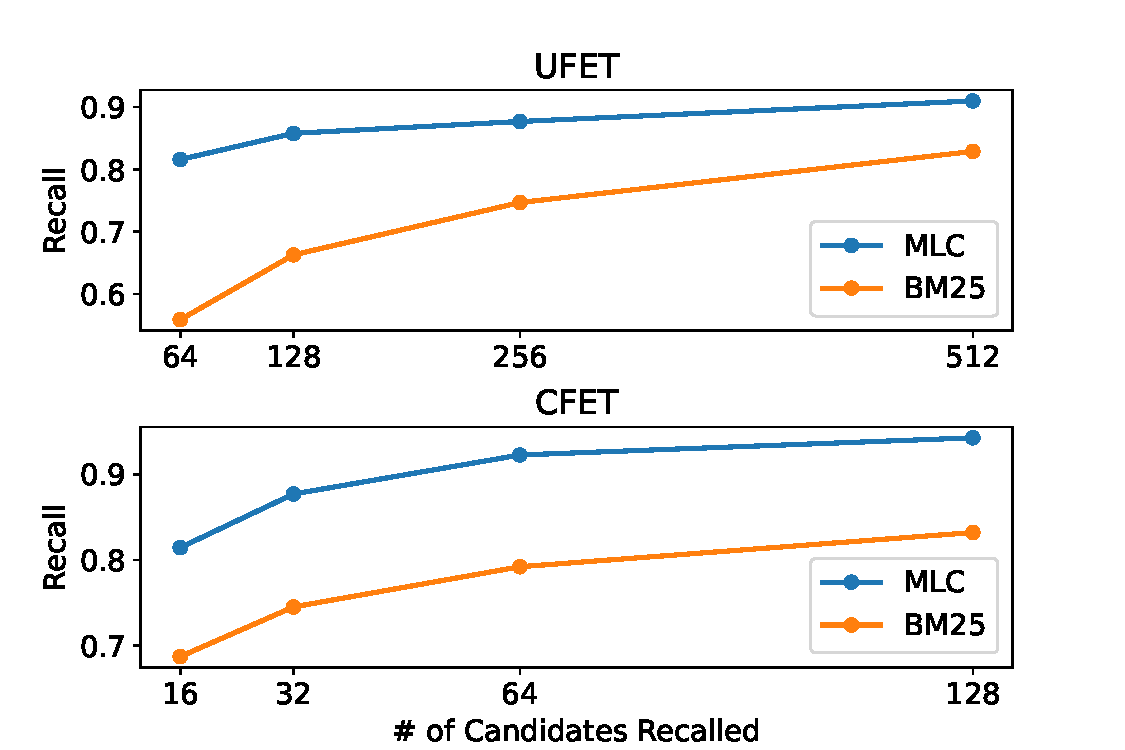
\includegraphics[width=\textwidth]{src/img/recall_compare_bm25.pdf}
         \label{fig:mb2}
     \end{subfigure}   
 \caption{Recall@$K$ of MLC and BM25.}
 \label{fig:recall}
\end{figure}

\subsection{Expand Stage}
\label{sec:expand}
In Table \ref{tab:expand}, we evaluate the F1 scores of all candidates expanded by exact match, and top-$10$ candidates expanded by the MLM using Bert-large. We also demonstrate the improvement of recall by using candidate expansion in Figure \ref{fig:expand_improvement}. On {\bf \textsc{UFET}} dataset, expanding around $32$ additional candidates based on $112$ MLC candidates results in $2\%$ higher recall compared to recalling all $128$ candidates by MLC. The recall of $128$ candidates after the expansion is comparable to the recall of $180$ candidates recalled from MLC. Similarly, expanding $10$ candidates is comparable to additionally recalling $80$ candidates using MLC.
In our experiments, we replace the last $48$ candidates recalled by MLC with the candidates recalled by MLM and Exact match for {\bf \textsc{UFET}} and $10$ for {\bf \textsc{CFET}}. We found the expand stage has a positive effect on the final performance of {\bf \textsc{\name}}s, and helps them reach SOTA performance (analyze in Sec. \ref{sec:analyze}).


\begin{table}[t]
\centering
\scalebox{0.75}{
\begin{tabular}{cccccc} 
\toprule
{\bf \textsc{Dataset}} & {\bf \textsc{Expand}} &   {\bf \textsc{P}}  & {\bf \textsc{R}}  &  {\bf \textsc{F1}} & \small{Avg \# Expanded}  \\ \midrule
\multirow{2}{*}{\bf \textsc{UFET}} & {\bf \textsc{Match}}      & 11.2   & 11.3     & 9.8    & 5.23     \\
      & {\bf \textsc{MLM}}  &  8.5     &   17.1   &  10.7  &    10    \\ \midrule
\multirow{2}{*}{\bf \textsc{CFET}} & {\bf \textsc{Match}}   &  11.4  &  14.5  & 11.2   & 4.57    \\
 & {\bf \textsc{MLM}}  & 21.3   &  19.5  & 17.7    & 10    \\ \midrule
\end{tabular}}
\caption{Evaluation of the recalled candidates.}
\label{tab:expand}
\end{table}
\begin{figure}[t]
     \centering
     \begin{subfigure}[h]{0.45\textwidth}
         \centering
         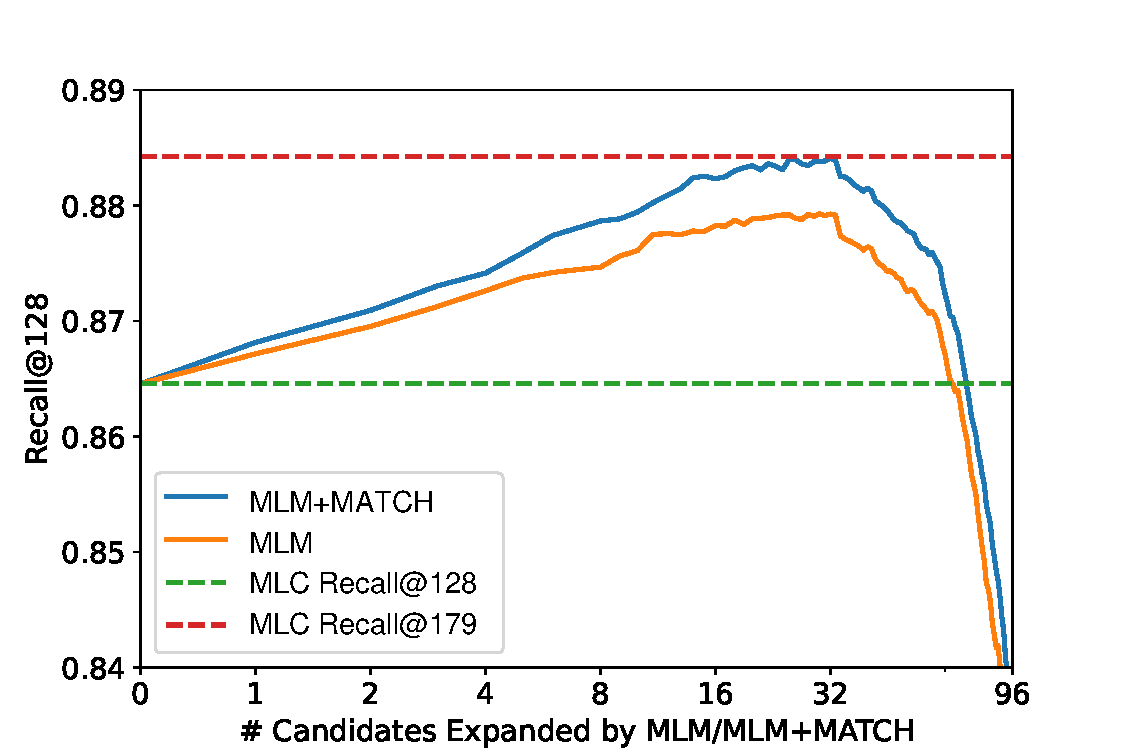
\includegraphics[width=\textwidth]{src/img/recall_ufet.pdf}
         \caption{Recall@$128$ on {\bf \textsc{UFET}} by including different number of expanded candidates. }
         \label{fig:c1}
     \end{subfigure}
     \vfill
     \begin{subfigure}[h]{0.45\textwidth}
         \centering
         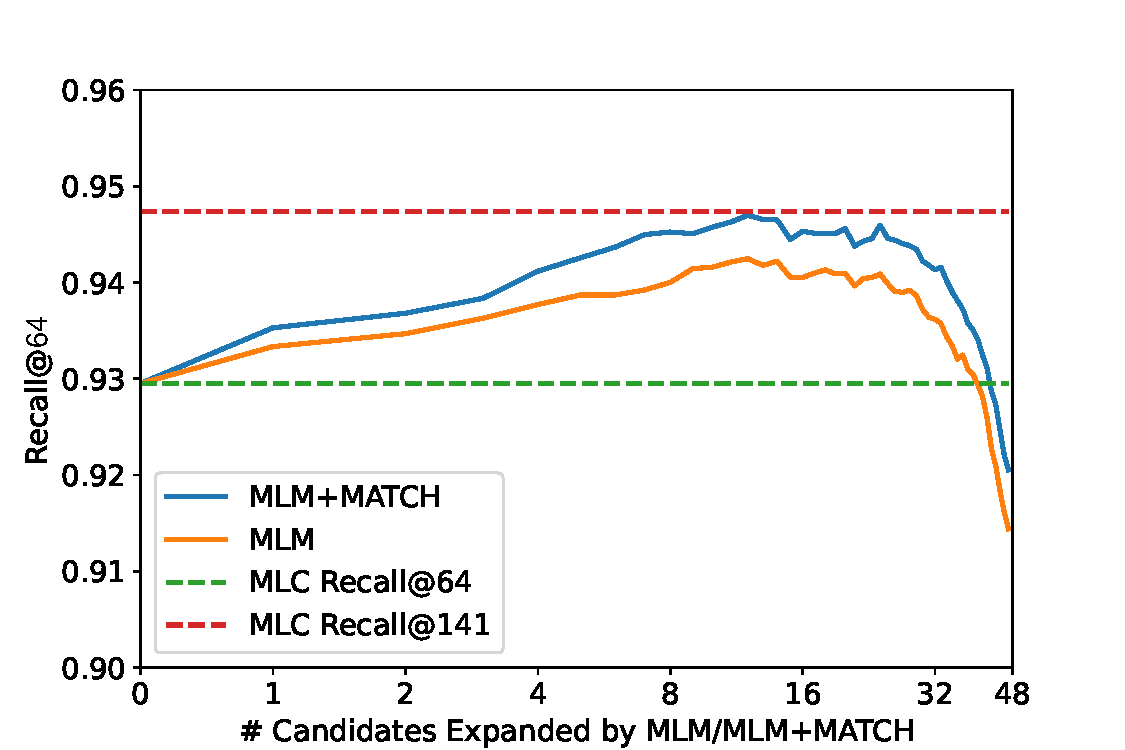
\includegraphics[width=\textwidth]{src/img/recall_cfet.pdf}
         \caption{Recall@$64$ on {\bf \textsc{CFET}} by including different number of expanded candidates.}
         \label{fig:c2}
     \end{subfigure}
\caption{Demonstration of the effect of expand stage. $x$-axis represents the number of candidates expanded by MLM/MLM+MATCH among these $128$ candidates. }
\label{fig:expand_improvement}
\end{figure}
\label{sec:exp_expand}
\subsection{Filter Stage and Final Results.}
\begin{table}[h!]
\centering
\scalebox{0.73}{
\renewcommand{\arraystretch}{1}
\begin{tabular}{cllll} \toprule
\multicolumn{2}{l}{\bf \textit{Base Models on UFET} }     & \bf \textsc{P}    & \bf \textsc{R}   & \bf \textsc{F1}  \\ \midrule
\multicolumn{5}{l}{\emph{MLC-like models}}        \\
\color{blue} \bf \texttt{B}& {\bf \textsc{Box4Types}}\cite{box4types}  & 52.8 & 38.8 & 44.8  \\
\color{blue}\bf \texttt{B}& {\bf \textsc{LDET}}$^\dagger$  \cite{onoe-durrett-2019-learning}          & 51.5 & 33.0 & 40.1 \\ 
\color{blue}\bf \texttt{B}& {\bf \textsc{MLMET}}$^\dagger$   {\cite{mlmet}}   & 53.6 & 45.3 & 49.1  \\
\color{blue}\bf \texttt{B}& {\bf \textsc{PL}}  \cite{ding2021prompt}   & 57.8 & 40.7 & 47.7 \\
\color{blue}\bf \texttt{B}& {\bf \textsc{DFET}}    \cite{dfet}      & 55.6 & 44.7 & 49.5 \\
\color{blue}\bf \texttt{B}& {\bf \textsc{MLC}} (reimplemented by us) & 46.5 & 34.9 & 39.9 \\ 
\color{red}\bf \texttt{R}& {\bf \textsc{MLC}} (reimplemented by us) & 42.2 & 44.9 & 43.5 \\ \hline 
\multicolumn{5}{l}{\emph{Seq2seq based models}}      \\
\color{blue}\bf \texttt{B} & {\bf \textsc{LRN} }  {\cite{liu-etal-2021-fine}}              & 54.5 & 38.9 & 45.4  \\\hline
\multicolumn{5}{l}{\emph{Filter models under our recall-expand-filter paradigm}}      \\
\color{blue}\bf \texttt{B} & {\bf \textsc{Vanilla CE}$_{128}$}   & 47.2 & 48.5 & 47.8 \\ 
\color{blue}\bf \texttt{B} & {\bf \textsc{\name-S$_{128}$}} (Ours)  & 53.2 & 48.3 & {\bf 50.6} \\ 
\color{blue}\bf \texttt{B} & {\bf \textsc{\name-S$_{128}$ w/o C2C}}   (Ours)   & 52.3 & 48.3 & 50.2 \\ 
\color{blue}\bf \texttt{B} & {\bf \textsc{\name-B$_{128}$}} (Ours)    & 49.9 & 50.0 & 49.9 \\ 
\color{blue}\bf \texttt{B} & {\bf \textsc{\name-B$_{128}$ w/o C2C}} (Ours)     & 49.9 & 48.2 & 49.0 \\ \hline
\color{red}\bf \texttt{R} & {\bf \textsc{Vanilla CE}$_{128}$}   & 49.6 & 49.0 & 49.3 \\ 
\color{red}\bf \texttt{R} & {\bf \textsc{\name-S$_{128}$}} (Ours)  & 53.3 & 47.3 & 50.1 \\ 
\color{red}\bf \texttt{R} & {\bf \textsc{\name-S$_{128}$ w/o C2C}}   (Ours)  & 53.2 & 46.6 & 49.7 \\ 
\color{red}\bf \texttt{R} & {\bf \textsc{\name-B$_{128}$}} (Ours)  & 52.5 & 47.9 & 50.1 \\ 
\color{red}\bf \texttt{R} & {\bf \textsc{\name-B$_{128}$ w/o C2C}} (Ours)     & 52.7 & 46.4 & 49.3 \\ \hline
\midrule
\multicolumn{2}{l}{\bf \textit{Large Models on UFET} }     & \bf \textsc{P}    & \bf \textsc{R}   & \bf \textsc{F1}  \\ \midrule
\multicolumn{5}{l}{\emph{MLC-like models}}        \\
\color{red}\bf \texttt{R} & {\bf \textsc{MLC}}  \cite{npcrf}               & 47.8 & 40.4 & 43.8  \\
\color{red}\bf \texttt{R} & {\bf \textsc{MLC-NPCRF}} \cite{npcrf}             & 48.7 & 45.5 & 47.0  \\
\color{red}\bf \texttt{R} & {\bf \textsc{MLC-GCN}} \cite{xiong-etal-2019-imposing}     & 51.2 & 41.0 & 45.5 \\
\color{blue}\bf \texttt{B} & {\bf \textsc{PL}}  \cite{ding2021prompt}       & 59.3 & 42.6 & 49.6  \\
\color{blue}\bf \texttt{B} & {\bf \textsc{PL-NPCRF}}  \cite{npcrf}  & 55.3 & 46.7 & {50.6}\\ \hline
\multicolumn{4}{l}{\emph{Cross-encoder based models and {\bf \textsc{\name}}s}}      \\
\color{red}\bf \texttt{R} & {\bf \textsc{LITE+L}}  \cite{lite}             & 48.7 & 45.8 & 47.2  \\
\color{teal}\bf \texttt{RM} & {\bf \textsc{LITE+NLI+L}} \cite{lite} & 52.4 & 48.9 & {50.6} \\ \hline
\multicolumn{4}{l}{\emph{Filter models under our recall-expand-filter paradigm}}   \\ 
\color{blue}\bf \texttt{B} & {\bf \textsc{Vanilla CE$_{128}$}}   & 50.3 & 49.6 & 49.9 \\ 
\color{blue}\bf \texttt{B} & {\bf \textsc{\name-S$_{128}$}}  (Ours)   & 52.5 & 49.1 & 50.8 \\ 
\color{blue}\bf \texttt{B} & {\bf \textsc{\name-S$_{128}$ w/o C2C}}   (Ours)   & 54.1 & 47.1 & 50.4 \\ 
\color{blue}\bf \texttt{B} & {\bf \textsc{\name-B$_{128}$}} (Ours)    & 54.0 & 48.6 & 51.2 \\ 
\color{blue}\bf \texttt{B} & {\bf \textsc{\name-B$_{128}$ w/o C2C}} (Ours)     & 52.8 & 48.3 & 50.4 \\ \hline
\color{red}\bf \texttt{R} & {\bf \textsc{Vanilla CE$_{128}$}}   & 54.5 & 49.3 & 51.8 \\ 
\color{red}\bf \texttt{R} & {\bf \textsc{\name-S$_{128}$}}  (Ours)   & 50.8 & 49.8  &  50.3 \\ 
\color{red}\bf \texttt{R} & {\bf \textsc{\name-S$_{128}$ w/o C2C}}   (Ours)   & 51.5 & 48.8 & 50.1 \\ 
\color{red}\bf \texttt{R} & {\bf \textsc{\name-B$_{128}$}} (Ours)    & 51.9 & 50.8 & 51.4 \\ 
\color{red}\bf \texttt{R} & {\bf \textsc{\name-B$_{128}$ w/o C2C}} (Ours)     & 51.6 & 51.6 & 51.6 \\ \hline
\color{teal}\bf \texttt{RM} & {\bf \textsc{\name-B$_{128}$ w/o C2C}} (Ours) & 56.3 & 48.5 & {\bf 52.1} \\ \hline
\midrule
\end{tabular}}
\caption{Macro-averaged UFET result. {\bf \textsc{LITE+L}} is LITE without NLI pretraining, {\bf \textsc{LITE+L+NLI}} is the full LITE model. Methods marked by $\dagger$ utilize either distantly supervised or augmented data for training. {\bf \textsc{\name-S$_{128}$}} denotes we use $128$ candidates recalled and expanded from the first two stages.}
\label{tab:ufet}
\end{table}
\begin{table}[t]
\centering
\scalebox{0.75}{
\renewcommand{\arraystretch}{1}
\begin{tabular}{cllll} \toprule
\multicolumn{2}{l}{\bf \textit{Models on CFET} }     & \bf \textsc{P}    & \bf \textsc{R}   & \bf \textsc{F1}  \\ \midrule
\multicolumn{5}{l}{\emph{MLC-like models}}        \\
\color{purple}\bf \texttt{N}& {\bf \textsc{MLC}} & 55.8 & 58.6 & 57.1 \\  
\color{purple}\bf \texttt{N}& {\bf \textsc{MLC-NPCRF}} \cite{npcrf}     & 57.0 & 60.5 & 58.7 \\ 
\color{purple}\bf \texttt{N}& {\bf \textsc{MLC-GCN}} \cite{xiong-etal-2019-imposing}   & 51.6 & 63.2 & 56.8 \\ 
\color{brown}\bf \texttt{C}& {\bf \textsc{MLC}} & 54.0 & 59.5 & 56.6 \\  
\color{brown}\bf \texttt{C}& {\bf \textsc{MLC-NPCRF}} \cite{npcrf}   & 54.0 & 61.6 & 57.3 \\  
\color{brown}\bf \texttt{C}& {\bf \textsc{MLC-GCN}} \cite{xiong-etal-2019-imposing} & 56.4 & 58.6 & 57.5 \\ \midrule 
\multicolumn{5}{l}{\emph{Filter models under our recall-expand-filter paradigm}}      \\
\color{purple}\bf \texttt{N} & {\bf \textsc{Vanilla CE}}   & 57.6 & 64.3 & 60.7 \\ 
\color{brown}\bf \texttt{C} & {\bf \textsc{Vanilla CE}}   & 54.0 & 63.3 & 58.3 \\  \hline
\color{purple}\bf \texttt{N} & {\bf \textsc{\name-S$_{64}$}} (Ours)  & 58.4 & 62.1 & 60.2 \\ 
\color{purple}\bf \texttt{N} & {\bf \textsc{\name-S$_{64}$ w/o C2C}}   (Ours)   & 59.1 & 61.5 & 60.3 \\ 
\color{purple}\bf \texttt{N} & {\bf \textsc{\name-B$_{64}$}} (Ours)    & 56.7 & 66.1 & 61.1 \\ 
\color{purple}\bf \texttt{N} & {\bf \textsc{\name-B$_{64}$ w/o C2C}} (Ours)     & 58.8 & 64.1 & 61.4 \\ \hline
\color{brown}\bf \texttt{C} & {\bf \textsc{\name-S$_{64}$}} (Ours)  & 55.5 & 62.6 & 58.8 \\ 
\color{brown}\bf \texttt{C} & {\bf \textsc{\name-S$_{64}$ w/o C2C}}   (Ours)   & 54.0 & 63.4 & 58.3 \\ 
\color{brown}\bf \texttt{C} & {\bf \textsc{\name-B$_{64}$}} (Ours)    & 55.0 & 63.5 & 59.0 \\ 
\color{brown}\bf \texttt{C} & {\bf \textsc{\name-B$_{64}$ w/o C2C}} (Ours)     & 57.3 & 61.3 & 59.3 \\ \hline
\midrule
\end{tabular}}
\caption{Macro-averaged CFET result.}
\label{tab:cfet}
\end{table}

In this section, we report the performance of {\bf \textsc{MCCE}} variants as the filter models and compare them with various strong baselines that we will introduce later. We also compare the inference speed of different models in this section. For filter models, we treat the number of candidates $K$ recalled and expanded by the first two stages as hyper-parameters, and tune it on the development set. We found the choice of PLM backbones has a non-negligible effect on the performance, and the PLM backbone of previous methods varies. Therefore for fairer comparisons to baselines, we conduct experiments of {\bf \textsc{\name}} using different backbone PLMs for our {\bf \textsc{\name}} models and report the results. For all {\bf \textsc{\name}} models, we use AdamW optimizer with a learning rate tuned between $5\times 10^{-6}$ and $2\times 10^{-5}$. The batch size we use is $4$ and we train the models for at most $50$ epochs with early stopping. {\bf \textsc{UFET}} also provides a large dataset obtained from distant supervision such as entity linking, we do not use it and only train and evaluate our models on human-labeled data.
\paragraph{Baselines}
The {\bf \textsc{MLC}} model we used for the recall stage and the cross-encoder ({\bf \textsc{CE}}) we introduced in Sec. \ref{sec:vanilla_ce} are natural baselines. We also compare our methods with recent PLM-based methods. {\bf \textsc{LDET} }\cite{onoe-durrett-2019-learning} is an MLC with Bert-base-uncased and ELMo \cite{elmo} trained on 727k examples automatically denoised from the distantly labeled UFET. {\bf \textsc{GCN} }\cite{xiong-etal-2019-imposing} uses GCN to model type correlations and obtain type embeddings. Types are scored by dot-product of mention and type embeddings. The original paper uses BiLSTM as the mention encoder and we use the results re-implemented by \citet{npcrf} using RoBERTa-large. {\bf \textsc{Box4Type} }\cite{box4types} uses Bert-large as the backbone and uses box embedding to encode mentions and types for training and inference. {\bf \textsc{LRN} }\cite{liu-etal-2021-fine} use Bert-base as the encoder and an LSTM decoder to generate types in a seq2seq manner. {\bf \textsc{MLMET} }\cite{mlmet} is a {\bf \textsc{MLC}} with Bert-base, but first pretrained by the distantly-labeled data augmented by masked word prediction, then finetuned and self-trained on the 2k human-annotated data. {\bf \textsc{PL}} \cite{ding2021prompt} uses prompt learning for entity typing. {\bf \textsc{DFET} }\cite{dfet} uses {\bf \textsc{PL}} as backbone and is a multi-round automatic denoising method for 2k labeled data. {\bf \textsc{LITE} }\cite{lite} is the previous SOTA system that formulates entity typing as textual inference. {\bf \textsc{LITE}} uses RoBERTa-large-MNLI as the backbone, and is a cross-encoder (introduced in Sec. \ref{sec:vanilla_ce}) with designed templates and a hierarchical loss. \citet{npcrf} proposes {\bf \textsc{NPCRF}} to enhance backbones such as {\bf \textsc{PL}} and {\bf \textsc{MLC}} by modeling type correlations, and reach performance comparable to {\bf \textsc{LITE}}.

\paragraph{Naming Conventions}
Let {\bf \textsc{\name-S}} be the {\bf \textsc{\name}} model that treats candidates as sub-tokens, and {\bf \textsc{\name-B}} be the model representing candidates as fixed-size blocks. The {\bf \textsc{\name}} model without {\bf \textsc{C2C}} attention (mentioned in Sec. \ref{sec:attn}) is denoted as {\bf \textsc{\name-B} w/o C2C}. For PLM backbones used in {\bf \textsc{UFET}}, we use {\color{blue} \bf \texttt{B}}, {\color{red} \bf \texttt{R}}, {\color{teal} \bf \texttt{RM}} to denote BERT-base-cased \cite{bert}, RoBERTa \cite{liu2019roberta}, and RoBERTa-MNLI \cite{liu2019roberta} respectively. For {\bf \textsc{CFET}}, we adopt two widely-used Chinese PLM, BERT-base-Chinese and NeZha-base-Chinese, and denote them as {\color{brown} \bf \texttt{C}} and {\color{purple} \bf \texttt{N}} respectively. 

\paragraph{UFET Results} We show the results of {\bf \textsc{UFET}} dataset in Table \ref{tab:ufet}. The results show that: (1) The recall-expand-filter paradigm is effective. Filter models outperform all baselines without the paradigm by a large margin. The vanilla CE under our paradigm reaches $51.8$ F1 compared to more complexed CE {\bf \textsc{LITE}} with $50.6$ F1 (2) {\bf \textsc{\name}} models reach SOTA performances. {\bf \textsc{\name-S$_{128}$}} with BERT-base performs best and reaches {\bf 50.6} F1 score, which is comparable to previous SOTA performance of large models such as {\bf \textsc{LITE+NLI+L}} and {\bf \textsc{PL+NPCRF}}. Among large models, {\bf \textsc{\name-B$_{128}$ w/o C2C}} also reaches SOTA performance with {\bf 52.1} F1 score. (3) {\bf \textsc{C2C}} attention is not necessary on large models, but is useful in base models. (4) Large models can utilize type semantics better. We found {\bf \textsc{\name-B}} outperforms {\bf \textsc{\name-S}} on large models, but underperforms {\bf \textsc{\name-S}} on base models. (5) Backbone PLM matters. We found the performance of {\bf \textsc{Vannila CE}} under our paradigm is largely affected by the PLM it used. It reaches $47.8$ F1 with BERT-base and $51.8$ F1 with RoBERTa-large. For {\bf \textsc{\name}} models, we found {\bf \textsc{\name}} performs better than {\bf \textsc{\name-B}} with BERT, and worse than {\bf \textsc{\name-B}} with RoBERTa. 

\begin{table*}[t]
\centering
\scalebox{0.9}{
\begin{tabular}{lllcc} \toprule
\bf \textsc{Model}  & \bf \textsc{\# FP} & \bf \textsc{Attn} & \bf \textsc{sents/sec} & \bf \textsc{F1} \\ \midrule
{\bf \textsc{MLC}} & \small{$1$}  & \small{$L_S^2D$} & 58.8 & 43.8\\
{\bf \textsc{LITE+NLI+L (CE)}}  & \small{$N$}  & \small{$L_S^2D$} & 0.02 & 50.6\\ \midrule \hline
\multicolumn{5}{l}{\emph{filter stage inference speed.}}  \\
{\bf \textsc{Vanilla CE$_{128}$}}  & \small{$128$}  & \small{$L_S^2D$} & 1.64 & 51.8 \\ 
{\bf \textsc{\name-S$_{128}$}}  & \small{$1$}  & \small{$(L_S+128)^2D$} & 60.8 & 50.1 \\ 
{\bf \textsc{\name-B$_{128}$}}  & \small{$1$}  & \small{$(L_S+128B)^2D$} & 22.3 & 51.4\\ 
{\bf \textsc{\name-B$_{128}$ w/o C2C}}  & \small{$1$}  & \small{$(L_S^2+256L_S B + 128 B^2)D$} & 25.2 & {\bf 52.1}\\ \bottomrule
\end{tabular}}
\caption{Inference speed comparison of models. {\bf \textsc{\# FP}} means the number of PLM forward passes required by a single inference. {\bf \textsc{ATTN}} column lists the theoretical attention complexity.  We also report the practical inference speed {\bf \textsc{sents/sec}} and the {\bf \textsc{F1}} scores on {\bf \textsc{UFET}} with RoBERTa-large architecture.}
\label{tab:speed}
\end{table*}

\begin{table}[t]
\centering
\scalebox{0.85}{
\renewcommand{\arraystretch}{1}
\begin{tabular}{cllll} \toprule
\multicolumn{2}{l}{\bf \textit{Models} }     & \bf \textsc{P}    & \bf \textsc{R}   & \bf \textsc{F1}  \\ \midrule
\multicolumn{5}{l}{\emph{coarse (9 types) Open Entity}}        \\ \hline
\color{red}\bf \texttt{R} & {\bf \textsc{MLC}}   & 76.8 & 78.5 & 77.6 \\ 
\color{red}\bf \texttt{R} & {\bf \textsc{Vanilla CE$_{9}$}}   & 82.3 & 81.0 & 81.6 \\ 
\color{red}\bf \texttt{R} & {\bf \textsc{\name-S$_{9}$}}   & 77.0 & 87.7 & 82.0 \\ 
\color{red}\bf \texttt{R} & {\bf \textsc{\name-B$_{9}$ w/o C2C}}   & 77.2 & 85.4 & 81.1 \\ \hline
\multicolumn{5}{l}{\emph{fine (130 types)}}        \\ \hline
\color{red}\bf \texttt{R} & {\bf \textsc{MLC}}   & 70.4 & 63.7 & 66.9  \\ 
\color{red}\bf \texttt{R} & {\bf \textsc{Vanilla CE}$_{130}$}   & 67.9 & 66.4 & 67.1 \\ 
\color{red}\bf \texttt{R} & {\bf \textsc{\name-S$_{130}$}}   & 65.8 & 71.8 & 68.7 \\ 
\color{red}\bf \texttt{R} & {\bf \textsc{\name-B$_{130}$ w/o C2C}}   & 64.1 & 70.5 & 67.1 \\ \hline
\midrule
\end{tabular}}
\caption{Micro-averaged results on UFET fine and coarse.}
\label{tab:ufet-coarse-fine}
\end{table}

\paragraph{CFET Results} We conduct experiments on {\bf \textsc{CFET}} and compare {\bf \textsc{\name}} models with several strong baselines:  {\bf \textsc{NPCRF}} and {\bf \textsc{GCN}} with MLC-like architecture, and {\bf \textsc{Vanilla CE}} under out paradigm which is proved to be better than {\bf \textsc{LITE}} on {\bf \textsc{UFET}}. The results are shown in Table \ref{tab:cfet}. Similar to results in {\bf \textsc{UFET}}, filter models under our paradigm significantly outperform MLC-like baselines, $+2.0$ F1 for Nezha-base and $+1.8$ F1 for BERT-base-Chinese. In {\bf \textsc{CFET}}, {\bf \textsc{\name}-B} is significantly better than {\bf \textsc{\name}-S}, on both Nezha-base and BERT-base-Chinese, indicating the importance of type semantics in Chinese language. We also find that {\bf \textsc{\name} w/o C2C} is generally better than  {\bf \textsc{\name} w/ C2C}, it is possibly because the C2C attention distracts the candidates from attending to mention and contexts.
\paragraph{Speed Comparison} Table \ref{tab:speed} shows the theoretical inference complexity (number of PLM forward passes, and attention complexity), and practical inference speed (number of sentences inferred per second) of different models. We conduct the speed test using NVIDIA TITAN RTX for all models, and the inference batch size is 4.
At the filter stage, the inference speed of {\bf \textsc{\name-S}} is on par with {\bf \textsc{MLC}} (even slightly faster because we don't need to score all types), and is about 40 times faster than {\bf \textsc{Vannila CE}} and thousands of times faster than {\bf \textsc{LITE}}. {\bf \textsc{\name-B w/o C2C}} is not significantly faster than {\bf \textsc{\name-B}} as expected. It's possibly because the computation related to the block attention is not fully optimized by existing deep learning frameworks. The speed advantage of {\bf \textsc{\name-B w/o C2C}} over {\bf \textsc{\name-B}} will be greater with more candidates.


\subsection{Fine-grained and Coarse-grained Entity Typing}
We also conduct experiments on Fine-grained (130-class) and Coarse-grained (9-class, also known as ``Open Entity'') entity typing, and the results are shown in Table \ref{tab:ufet-coarse-fine}. As the type candidate set is much smaller in these settings, we skip the recall and expand stages and directly run the filter models and compare them to baselines. Results show that both {\bf \textsc{\name}-S} and {\bf \textsc{\name}-B} are still better than {\bf \textsc{MLC}} and {\bf \textsc{Vanilla CE}}, and {\bf \textsc{\name}-S} is better than {\bf \textsc{\name}-B} on coarser-grained cases possibly because the coarser-grained types are simpler in surface-forms and {\bf \textsc{\name}-S} will not lose many type semantics.






\section{Discussion}
\label{ss: discussion}

In this section, we discuss how security scanners can defend against evasions (Section~\ref{ss:anti-evasion})
and what limitations our work currently has (Section~\ref{ss:extension}).

\subsection{Mitigating Evasions}
\label{ss:anti-evasion}

One way to mitigate dynamic evasions is to adapt general anti-evasion techniques from other domains to the problem of analyzing PDF documents.
Several recent papers propose to load a potentially malicious file in environments targeted at revealing the malicious behavior of the file.
For example, FuzzDroid~\cite{rasthofer2017making}, IntelliDroid~\cite{wong2016intellidroid}, and SmartDroid~\cite{zheng2012smartdroid} try to cause a potentially malicious Android app to reach ``sensitive'' API calls that would reveal malicious behavior, such as sending an SMS to a premium number.
Adapting this technique to PDF scanners requires identifying sensitive APIs in PDFs.
For known exploits, such APIs may be known, e.g., it is known that the ``Toolbutton'' exploit relies on calling the \code{app.addToolButton} API.
Finding sensitive APIs for previously unknown exploits remains an open research problem.
A related technique to cope with dynamic evasions is to explore multiple execution paths for branch decisions that depend on the environment in which a file is executed.
Rozzle~\cite{rozzle-de-cloaking-internet-malware-2} proposes this idea for client-side JavaScript code.
Adapting their approach is a promising direction for mitigating the environment-related dynamic evasions.

To deal with UI-related evasions, dynamic scanners could adapt ideas used in PuppetDroid~\cite{gianazza2014puppetdroid} and PyTrigger~\cite{fleck2013pytrigger}.
These approaches record an interaction trace from a human and play it back when loading the file under analysis to get through possible checks that guard the attack.
One of the dynamic scanners studied in this work, Cuckoo, mitigates evasions using a simpler form of this idea: The scanner arbitrarily moves the mouse to simulate a human user~\cite{cuckoo_mouse_movement}.
However, this mitigation technique is unlikely to work for evasions that require a more complicated user interaction, such as a ``captcha''.

To identify files that behave differently in an analysis environment, some techniques compare the execution behavior of the file in several different environments, e.g. virtual and physical~\cite{balzarotti2010efficient}.
Another kind of anti-evasion technique is to hide any difference between a virtual and a physical execution environment to fool the evasive malware~\cite{shi2018handling}.
%
Finally, to deal with the large number of possible evasions and combinations of evasions, training machine learning models to distinguish benign from malicious files seems to be a worthwhile direction~\cite{smutz2012malicious,vsrndic2013detection,laskov2011static,corona2014lux0r}.
The main challenge for effectively training machine learning models is to obtain a sufficiently large set of labeled data.
Our framework could serve as a generator of malicious training files that use different evasions and combinations of evasions.

The high recall of SAFE-PDF~\cite{2018arXiv181012490J}, which is based on abstract interpretation of JavaScript code embedded in PDFs, shows that conservative program analysis may provide an effective way of detecting malicious behavior despite evasions. The downside of any conservative program analysis are spurious warnings, which the relatively high false positive ratio of SAFE-PDF confirms.



\subsection{Choice of Scanners}
\label{ss:extension}

We focus on in-production, commercial security scanners because they represent the current state-of-the-practice, and recent academic scanners because they represent the state-of-the-art.
The studied scanners contain more static than dynamic scanners because static scanners currently dominate the market.
For example, the VirusTotal service aggregates more than 60 static scanners at the time of writing this paper~\cite{vt_engines_count}, whereas we could find only ten commercial dynamic scanners, out of which three consented to participate in this research.

Our work should not be understood as a comparison of different scanners, but rather as a comparison of each scanner's effectiveness before and after adding evasions.
The version of the scanners used in online aggregation services, which we use for the studied static scanners, may differ from the full-fledged scanners, because vendors may optimize the response time for an online service~\cite{pitfall}.



%\newpage
\bibliography{library,library_mh}

\beginsupplement

\newpage

\appendix

\section*{Appendix}

\section{Self-organizing maps}\label{sec:SOMs}

The general idea of a self-organizing map (SOM) is to approximate a data manifold in a high-dimensional continuous space with a lower dimensional discrete one \citep{Kohonen1998}.
It can therefore be seen as a nonlinear discrete dimensionality reduction.
The mapping is achieved by a procedure in which this discrete representation (the \emph{map}) is randomly embedded into the data space and then iteratively optimized to approach the data manifold more closely.

The map consists of $k$ nodes $V=\{v_1, \dots , v_k\}$, where every node corresponds to an embedding in the data space $e_v \in \mathbb{R}^d$ and a representation in the lower-dimensional discrete space $m_v \in M$, where usually $M \subset \mathbb{N}^2$.
There are two different geometrical measures that have to be considered during training: the neighborhood function $N(m_u, m_{\tilde{v}})$ that is defined on the low-dimensional map space and the Euclidean distance $D (e_u, e_{\tilde{v}}) = \| e_u - e_{\tilde{v}} \|_2$ in the high-dimensional data space.
The SOM optimization tries to induce a coupling between these two properties, such that the topological structure of the representation reflects the geometrical structure of the data.


\begin{algorithm}
\caption{Self-organizing map training}
\label{alg:som_train}

\begin{algorithmic}
	\Require data set $\mathcal{D} = \{x_1, \dots ,x_n \; \vert \; x_i \in \mathbb{R}^d\}$, number of nodes $k$, neighborhood function $N(\cdot)$, step size $\eta$
	\State initialize set of $k$ nodes $V=\{v_1, \dots , v_k\}$
	\State initialize embeddings $e_v \in \mathbb{R}^d \; \forall \; v \in V$
	\While{not converged}
	\ForAll {$x_i \in \mathcal{D}$}
		\State find the closest SOM node $\tilde{v} := \argmin_{v \in V} \| x_i - e_v \|_2$
		\State update node embedding $e_{\tilde{v}} \gets e_{\tilde{v}} + \eta \, (x_i - e_{\tilde{v}})$
		\ForAll {$u \in V \backslash \tilde{v}$}
			\State update neighbor embedding $e_u \gets e_u + \eta \, N(m_{\tilde{v}}, m_u) (x_i - e_u)$
		\EndFor
	\EndFor
	\EndWhile
\end{algorithmic}
	
\end{algorithm}

The SOM training procedure is described in Algorithm~\ref{alg:som_train}.
During training on a data set $\mathcal{D}$, a winner node $\tilde{v}$ is chosen for every point $x_i$ according to the Euclidean distance of the point and the node's embedding in the data space.
The embedding vector for the winner node is then updated by pulling it into the direction of the data point with some step size $\eta$.
The embedding vectors of the other nodes are also updated -- potentially with a smaller step size -- depending on whether they are neighbors of the winner node in the map space $M$.

The neighborhood is defined by the neighborhood function $N(m_u, m_{\tilde{v}})$.
There can be different design choices for the neighborhood function, e.g.\ rectangular grids, hexagonal grids or Gaussian neighborhoods.
For simplicity and ease of visualization, we usually choose a two-dimensional rectangular grid neighborhood in this paper.

In this original formulation of the SOM training, the nodes are updated one by one with a fixed step size.
In our model, however, we use a gradient-based optimization of their distances to the data points and update them in minibatches.
This leads to larger step sizes when they are farther away from the data and smaller step sizes when they are close.
Overall, our gradient-based SOM training seems to perform better than the original formulation (see Tab.~\ref{tab:performance}).

It also becomes evident from this procedure that it will be very hard for the map to fit disjoint manifolds in the data space.
Since the nodes of the SOM form a fully connected graph, they do not possess the ability to model spatial gaps in the data.
We overcome this problem in our work by mapping the data manifold with a variational autoencoder into a lower-dimensional latent space.
The VAE can then learn to close the aforementioned gaps and map the data onto a compact latent manifold, which can be more easily modeled with the SOM.



\section{Implementation details}\label{sec:implementation}

The hyperparameters of our model were optimized using Robust Bayesian Optimization with the packages \texttt{sacred} and \texttt{labwatch} \citep{Greff2017a} for the parameter handling and \texttt{RoBo} \citep{Klein2017} for the optimization, using the mean squared reconstruction error as the optimization criterion.
Especially the weighting hyperparameters $\alpha, \beta, \gamma$ and $\tau$ (see Eq.~\eqref{eq:L_somvae} and Eq.~\eqref{eq:L_prob}) have to be tuned carefully, such that the different parts of the model converge at roughly the same rate.
We found that 2000 steps of Bayesian optimization sufficed to yield a performant hyperparameter assignment.

Since our model defines a general framework, some competitor models can be seen as special cases of our model, where certain parts of the loss function are set to zero or parts of the architecture are omitted.
We used the same hyperparameters for those models.
For external competitor methods, we used the hyperparameters from the respective publications where applicable and otherwise the default parameters from their packages.
The models were implemented in TensorFlow \citep{GoogleResearch2015} and optimized using Adam \citep{Kingma2015}.


\section{Clustering performance measures}\label{sec:clustering_performance}

Given that one of our most interesting tasks at hand is the clustering of data, we need some performance measures to objectively compare the quality of this clustering with other methods.
The measures that we decided to use and that have been used extensively in the literature are \emph{purity} and \emph{normalized mutual information} (NMI) \citep{Manning2008}.
We briefly review them in the following.

Let the set of ground truth classes in the data be $C = \{ c_1, c_2, \dots, c_J \}$ and the set of clusters that result from the algorithm $\Omega = \{ \omega_1, \omega_2, \dots, \omega_K \}$.
The \emph{purity} $\pi$ is then defined as $\pi(C, \Omega) = \frac{1}{N} \sum_{k = 1}^K \max_j \vert \omega_k \cap c_j \vert$ where $N$ is the total number of data points.
Intuitively, the purity is the accuracy of the classifier that assigns the most prominent class label in each cluster to all of its respective data points.

While the purity has a very simple interpretation, it also has some shortcomings.
One can for instance easily observe that a clustering with $K = N$, i.e.\ one cluster for every single data point, will yield a purity of $1.0$ but still probably not be very informative for most tasks.
It would therefore be more sensible to have another measure that penalizes the number of clusters.
The normalized mutual information is one such measure.

The NMI is defined as $\textit{NMI}(C, \Omega) = \frac{2 \; I(C, \Omega)}{H(C) + H(\Omega)}$ where $I(C, \Omega)$ is the mutual information between $C$ and $\Omega$ and $H(\cdot)$ is the Shannon information entropy.
While the entropy of the classes is a data-dependent constant, the entropy of the clustering increases with the number of clusters.
It can therefore be seen as a penalty term to regularize the trade-off between low intra-cluster variance and a small number of clusters.
Both NMI and purity are normalized, i.e.\ take values in $[0,1]$.



\section{Experimental details}


\subsection{Clustering on MNIST and Fashion-MNIST} \label{sec:mnist_appendix}

Additionally to the results in Table~\ref{tab:performance}, we performed experiments to assess the influence of the number of clusters $k$ on the clustering performance of our method.
We chose different values for $k$ between 4 and 64 and tested the clustering performance on MNIST and Fashion-MNIST (Tab.~\ref{tab:k_performance}).

\begin{table}
    \centering
    \caption{Performance comparison of our method with different numbers of clusters in terms of purity and normalized mutual information on different benchmark data sets. The values are the means of 10 runs and the respective standard errors.}
    \begin{tabular}{lrrrr}
        \toprule
         & \multicolumn{2}{c}{MNIST} & \multicolumn{2}{c}{Fashion-MNIST} \\
        \cmidrule(rl){2-3}
        \cmidrule(rl){4-5}
        Number of clusters & \multicolumn{1}{c}{Purity} & \multicolumn{1}{c}{NMI} & \multicolumn{1}{c}{Purity} & \multicolumn{1}{c}{NMI} \\
         \midrule
         $k = 4$ & 0.364 $\pm$ 0.009 & 0.378 $\pm$ 0.018 & 0.359 $\pm$ 0.005 & 0.431 $\pm$ 0.008\\
         $k = 9$ & 0.626 $\pm$ 0.006 & 0.554 $\pm$ 0.004 & 0.558 $\pm$ 0.007 & 0.560 $\pm$ 0.006\\
         $k = 16$ & 0.721 $\pm$ 0.006 & 0.587 $\pm$ 0.003 & 0.684 $\pm$ 0.003 & \textbf{0.589 $\pm$ 0.003}\\
         $k = 25$ & 0.803 $\pm$ 0.003 & \textbf{0.613 $\pm$ 0.002} & 0.710 $\pm$ 0.003 & 0.572 $\pm$ 0.002\\
         $k = 36$ & 0.850 $\pm$ 0.002 & \textbf{0.612 $\pm$ 0.001} & 0.732 $\pm$ 0.002 & 0.556 $\pm$ 0.002\\
         $k = 49$ & 0.875 $\pm$ 0.002 & 0.608 $\pm$ 0.001 & 0.750 $\pm$ 0.002 & 0.545 $\pm$ 0.001\\
         $k = 64$ & \textbf{0.894 $\pm$ 0.002} & 0.599 $\pm$ 0.001 & \textbf{0.758 $\pm$ 0.002} & 0.532 $\pm$ 0.001\\
         \bottomrule
    \end{tabular}
    \label{tab:k_performance}
\end{table}

It can be seen that the purity increases monotonically with $k$, since it does not penalize larger numbers of clusters (see Sec.~\ref{sec:clustering_performance}).
The NMI, however, includes an automatic penalty for misspecifying the model with too many clusters.
It therefore increases first, but then decreases again for too large values of $k$.
The optimal $k$ according to the NMI seems to lie between 16 and 36.


\subsection{Interpretable representations of chaotic time series}\label{sec:lorenz_appendix}

The Lorenz system is the system of coupled ordinary differential equations defined by
%
\begin{equation*}
	\frac{dX}{dt} = a (Y - X) \hskip 4em
	\frac{dY}{dt} = X (b - Z) - Y \hskip 4em
	\frac{dZ}{dt} = XY - cZ
\end{equation*}
%
with tuning parameters $a$, $b$ and $c$. For parameter choices $a = 10$, $b = 28$ and $c = \frac{8}{3}$, the system shows chaotic behavior by forming a strange attractor \citep{Tucker1999} with the two attractor points being given by $p_{1,2} = \lbrack \pm \sqrt{c (b-1)}, \pm \sqrt{c (b-1)}, b-1 \rbrack^T$.

We simulated 100 trajectories of 10,000 time steps each from the chaotic system and trained the SOM-VAE as well as k-means on it with 64 clusters/embeddings respectively.
The system chaotically switches back and forth between the two attractor basins.
By computing the Euclidian distance between the current system state and each of the attractor points $p_{1,2}$, we can identify the current attractor basin at each time point.

In order to assess the interpretability of the learned representations, we have to define an objective measure of interpretability.
We define interpretability as the similarity between the representation and the system's ground truth macro-state.
Since representations at single time points are meaningless with respect to this measure, we compare the evolution of representations and system state over time in terms of their entropy.

We divided the simulated trajectories from our test set into spans of 100 time steps each.
For every subtrajectory, we computed the entropies of those subtrajectories in the real system space (macro-state and noise), the assigned attractor basin space (noise-free ground-truth macro-state), the SOM-VAE representation and the k-means representation.
We also observed for every subtrajectory whether or not a change between attractor basins has taken place.
Note that the attractor assignments and representations are discrete, while the real system space is continuous.
In order to make the entropies comparable, we discretize the system space into unit hypercubes for the entropy computation.
For a representation $\mathcal{R}$ with assignments $\mathcal{R}_t$ at time $t$ and starting time $t_{start}$ of the subtrajectory, the entropies are defined as
%
\begin{equation}
	H \left( \mathcal{R}, t_{start} \right) = H \left( \lbrace R_t \; \vert \; t_{start} \leq t < t_{start} + 100 \rbrace \right)
\end{equation}
%
with $H(\cdot)$ being the Shannon information entropy of a discrete set.


\subsection{Learning representations of acute physiological states in the ICU}\label{sec:ICU_appendix}

All experiments were performed on dynamic data extracted from the \texttt{eICU} Collaborative Research Database \citep{Goldberger2000}.
Irregularly sampled time series data were extracted from the raw tables and then resampled to a regular time grid using a combination of forward filling and missing value imputation using global population statistics.
We chose a grid interval of one hour to capture the rapid dynamics of patients in the ICU.

Each sample in the time-grid was then labeled using a dynamic variant of the \texttt{APACHE} score \citep{Knaus1985}, which is a proxy for the instantaneous physiological state of a patient in the ICU.
Specifically, the variables \texttt{MAP}, \texttt{Temperature}, \texttt{Respiratory rate}, \texttt{HCO3}, \texttt{Sodium}, \texttt{Potassium}, and \texttt{Creatinine} were selected from the score definition, because they could be easily defined for each sample in the \texttt{eICU} time series.
The value range of each variable was binned into ranges of normal and abnormal values, in line with the definition of the \texttt{APACHE} score, where a higher score for a variable is obtained for abnormally high or low values.
The scores were then summed up, and we define the predictive score as the \emph{worst (highest) score} in the next $t$ hours, for $t \in \{ 6, 12, 24 \}$.
Patients are thus stratified by their expected pathology in the near future, which corresponds closely to how a physician would perceive the state of a patient.
The training set consisted of 7000 unique patient stays, while the test set contained 3600 unique stays.


\subsection{Detailed analysis of \texttt{SOMVAEprob} patient states}
\label{subsec:detailed_icu}

As mentioned in the main text (see Fig \ref{fig:ICU_representations}) the \texttt{SOMVAEProb}
is able to uncover compact and interpretable structures in the latent space with respect
to future physiology scores. In this section we show results for acute physiology scores
in greater detail, analyze enrichment for future mortality risk, arguably the most
important severity indicator in the ICU, and explore phenotypes for particular 
physiological abnormalities.

% Acute physiology scores

\subsubsection*{Full results for future acute physiology scores}

\begin{figure}[h!]

\centering
\begin{subfigure}[t]{0.30\textwidth}
\centering
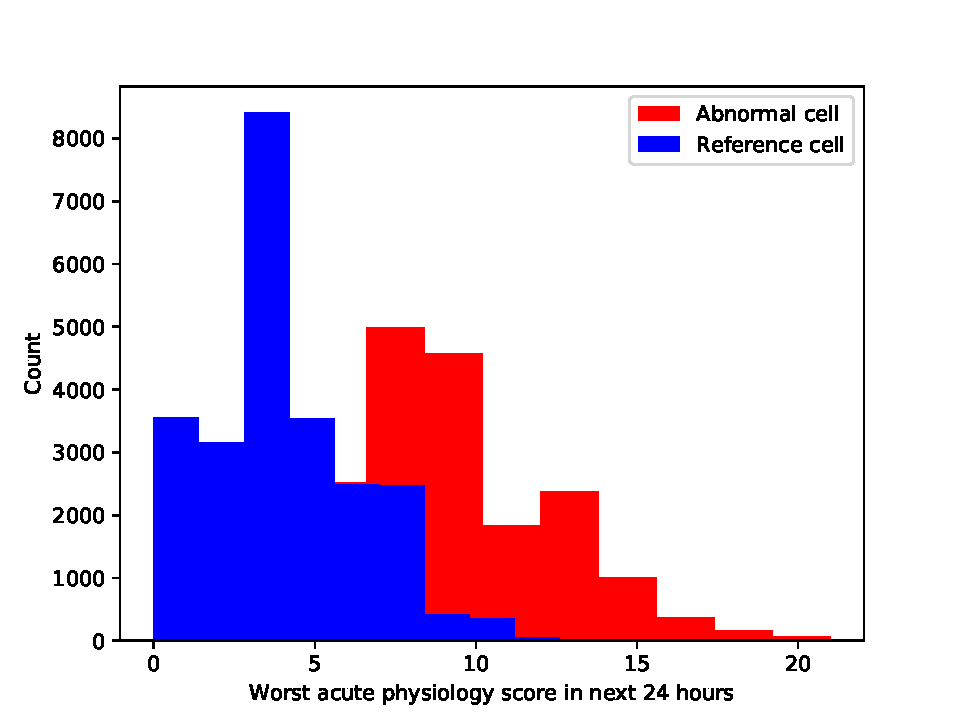
\includegraphics[scale=0.30]{./figures/icu_somvaeprob/distribution_cells}
\caption{Abnormal vs. reference cell}
\end{subfigure}
\begin{subfigure}[t]{0.30\textwidth}
\centering
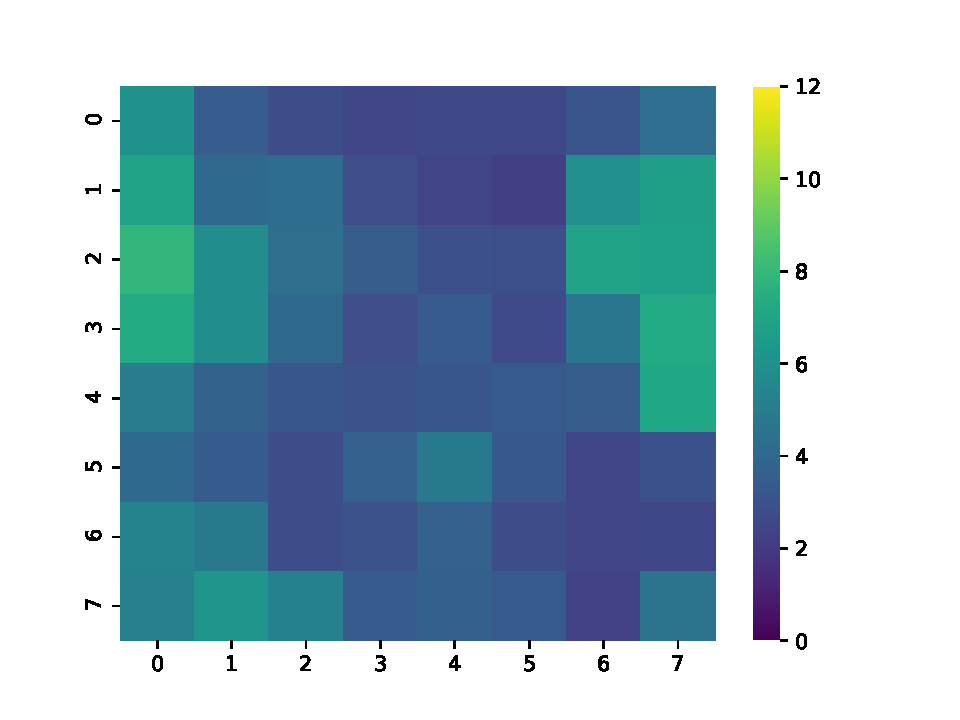
\includegraphics[scale=0.30]{./figures/icu_somvaeprob/detail_heatmaps_full_score_6}
\caption{Acute physiology score (6)}
\end{subfigure}
\begin{subfigure}[t]{0.30\textwidth}
\centering
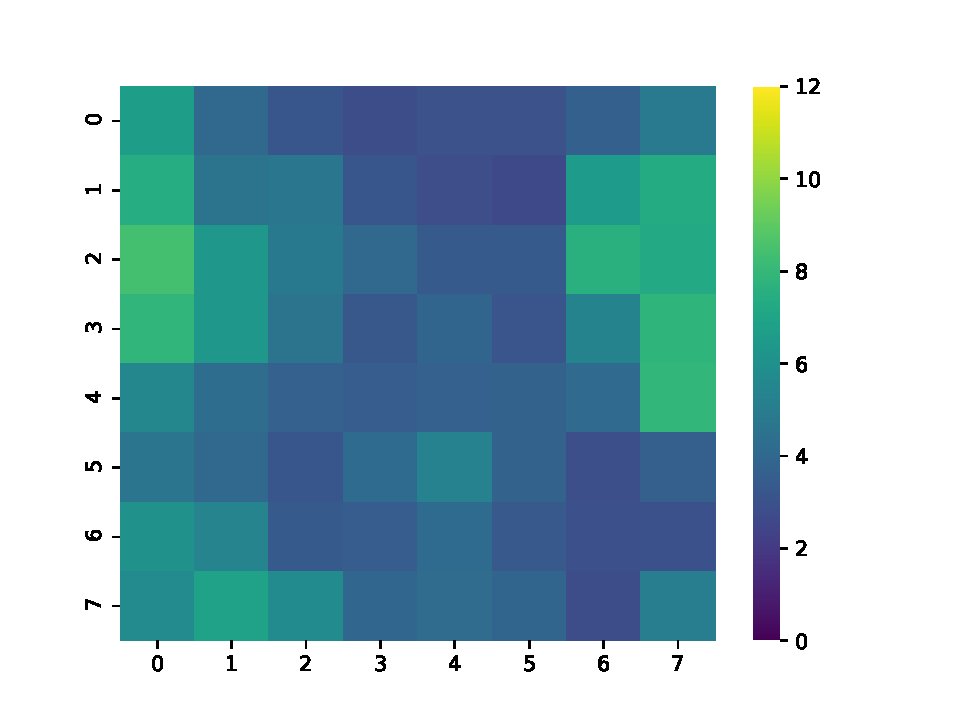
\includegraphics[scale=0.30]{./figures/icu_somvaeprob/detail_heatmaps_full_score_12}
\caption{ Acute physiology score (12)}
\end{subfigure}

\caption{(a) shows the difference in distribution of the acute
         physiology score in the next 24 hours, between time-points assigned to the most 
         abnormal cell in the \texttt{SOMVAEprob} map with coordinates [2,0] vs. 
         a normal cell chosen from the middle of the map with coordinates [4,3]. It is apparent that
         the distributions are largely disjoint, which means that the representation induced by 
         \texttt{SOMVAEprob} clearly distinguishes these risk profiles. Statistical tests for difference
         in distribution and location parameter are highly significant at p-values of $p \leq 10^{-3}$, as we
         have validated using a 2-sample $t$-test and Kolmogorov-Smirnov test. In (b-c) the enrichment 
         of the map for the mean acute physiology score in the next 6 and 12 hours is shown, for completeness.
         The enrichment patterns on the 3 maps, for the future horizons $\{6,12,24\}$, are almost identical, 
         which provides empirical evidence for the temporal stability of the \texttt{SOMVAEProb} embedding.}

\end{figure}

% Dynamic mortality in the next {12,24} hours

\subsubsection*{Dynamic mortality risk of patients on the \texttt{SOMVAEprob} map}

\begin{figure}[h!]
\centering
\begin{subfigure}[t]{0.47\textwidth}
\centering
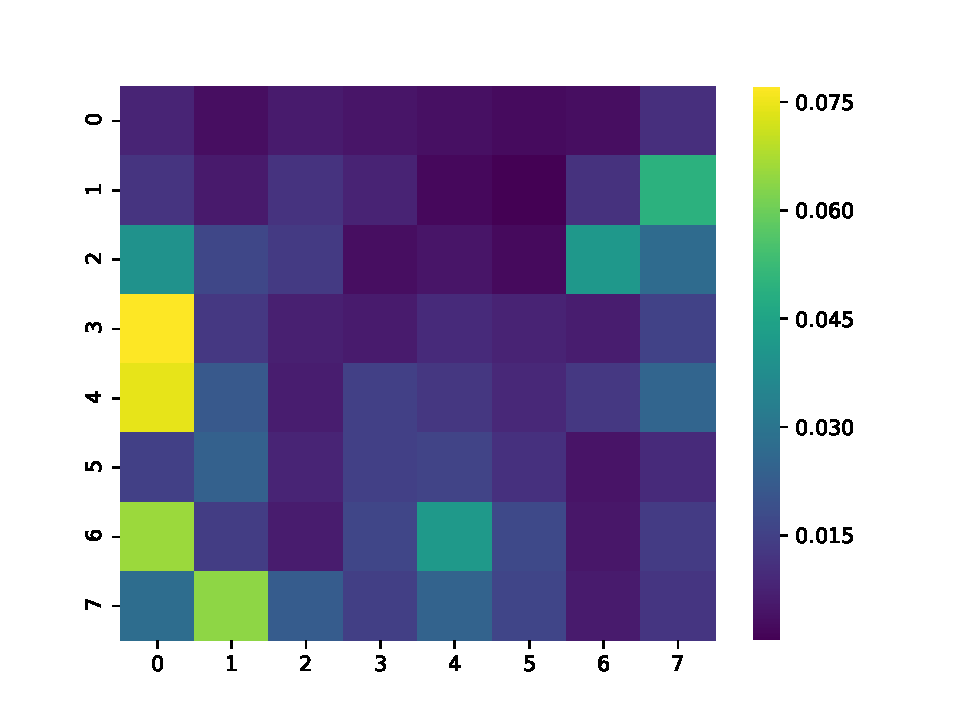
\includegraphics[scale=0.4]{./figures/icu_somvaeprob/detail_heatmaps_unit_discharge_expired_24}
\caption{24-hour mortality risk}
\end{subfigure}
\begin{subfigure}[t]{0.47\textwidth}
\centering
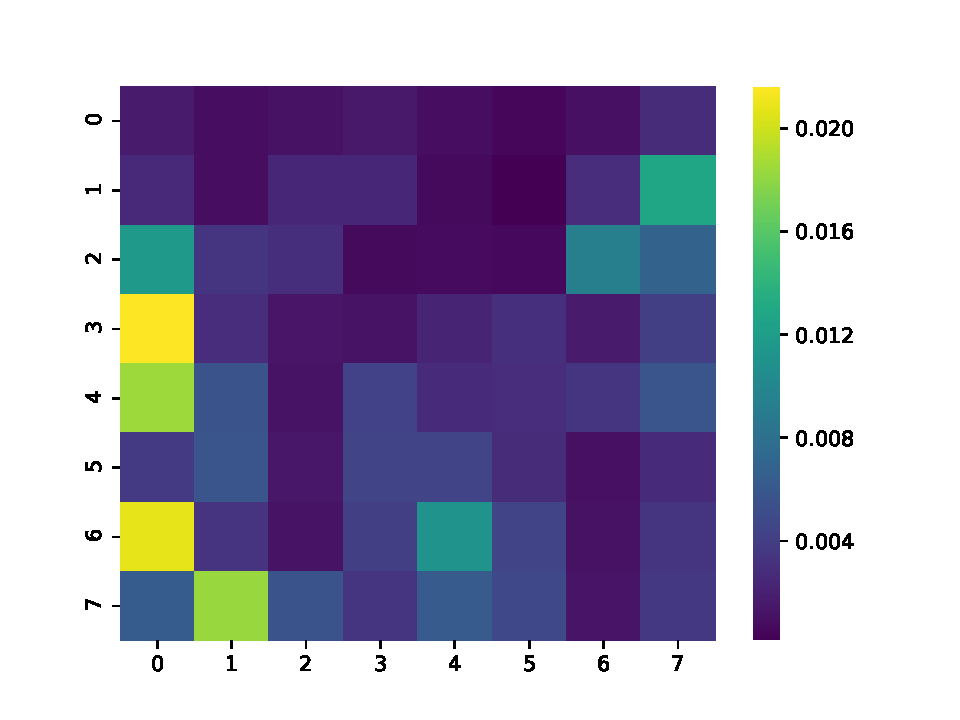
\includegraphics[scale=0.4]{./figures/icu_somvaeprob/detail_heatmaps_unit_discharge_expired_6}
\caption{6-hour mortality risk}
\end{subfigure}
\caption{(a) Dynamic mortality risk in the next 24 hours. (b) Short-term dynamic mortality risk in the next
             6 hours. We observe that the left-edge and right-edge regions of the \texttt{SOMVAEprob} map which
             are enriched for higher acute physiology scores (see Fig \ref{fig:ICU_representations}) also exhibit elevated 
             mortality rates over the baseline. Interestingly, according to future mortality risk, which is an important severity indicator,
             patients on the left-edge are significantly more sick on average than those on the right edge, which is
             less visible from the enrichment for acute physiology scores.}
\end{figure}

\newpage

% Detailed analysis of vital sign abnormalities

\subsubsection*{Patient state phenotypes on the \texttt{SOMVAEprob} map}

\begin{figure}[h!]
\centering
\begin{subfigure}[t]{0.22\textwidth}
\centering
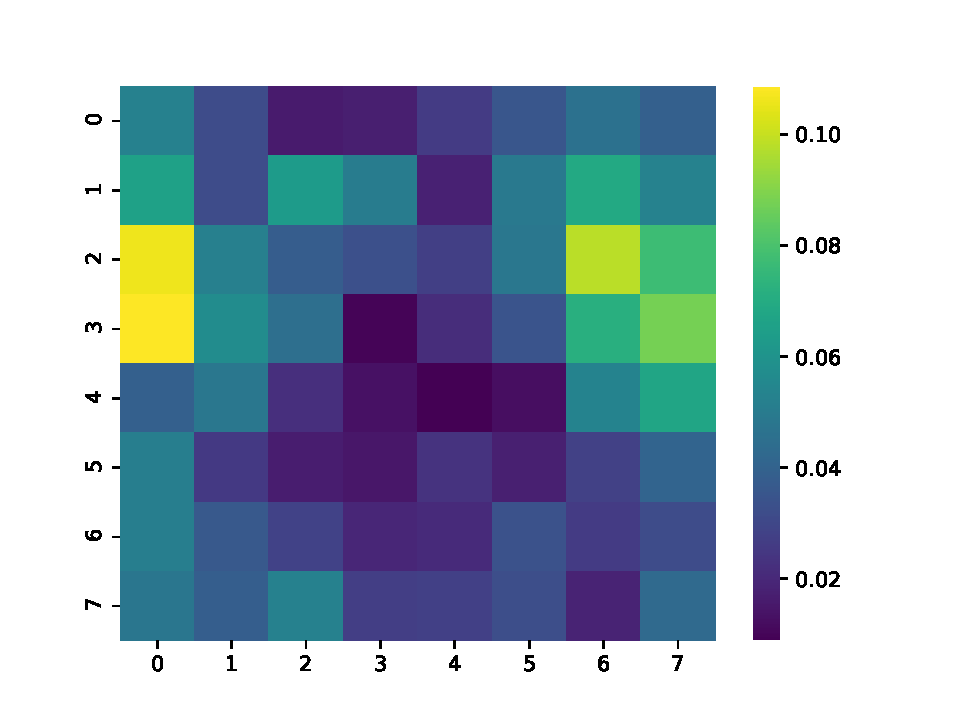
\includegraphics[scale=0.22]{./figures/icu_somvaeprob/detail_heatmaps_low_sodium}
\caption{Low Sodium}
\end{subfigure}
\begin{subfigure}[t]{0.22\textwidth}
\centering
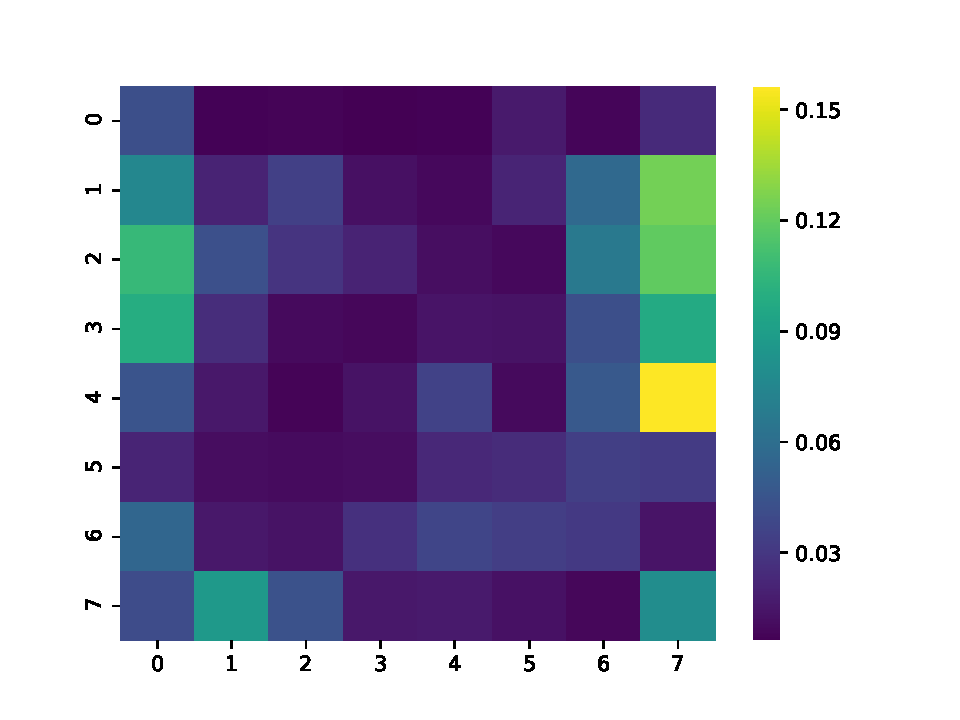
\includegraphics[scale=0.22]{./figures/icu_somvaeprob/detail_heatmaps_high_potassium}
\caption{High Potassium}
\end{subfigure}
\begin{subfigure}[t]{0.22\textwidth}
\centering
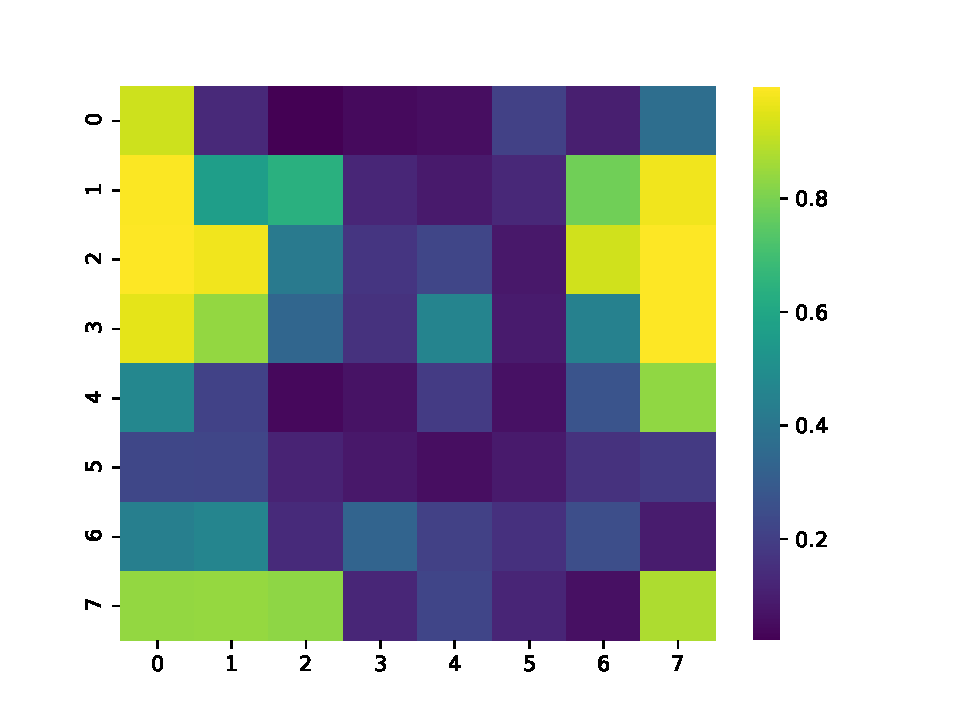
\includegraphics[scale=0.22]{./figures/icu_somvaeprob/detail_heatmaps_high_creatinine}
\caption{High Creatinine}
\end{subfigure}
\begin{subfigure}[t]{0.22\textwidth}
\centering
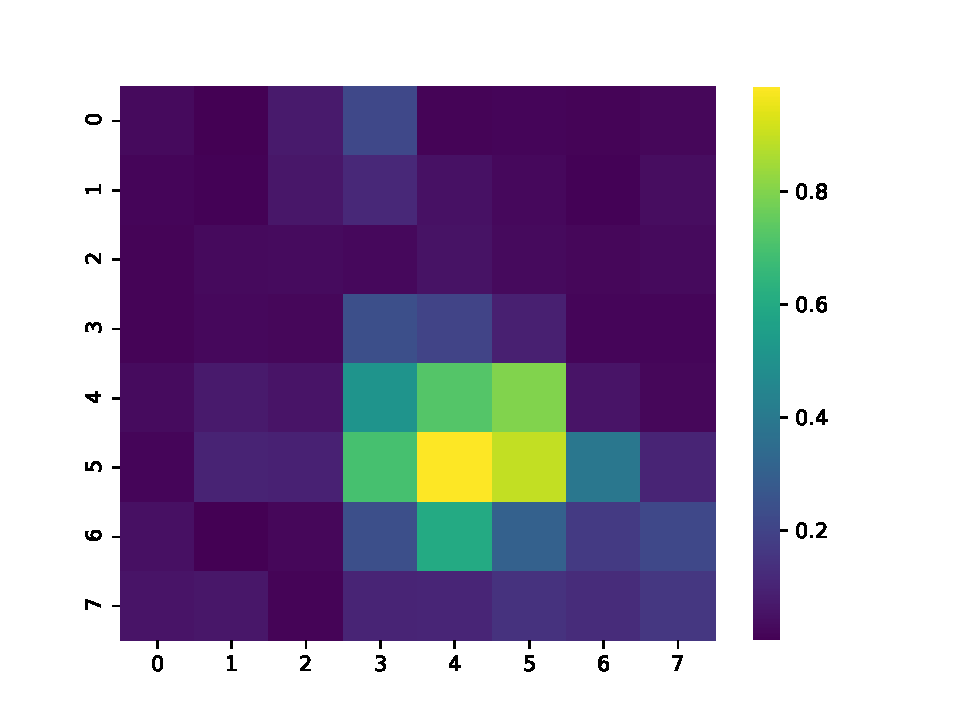
\includegraphics[scale=0.22]{./figures/icu_somvaeprob/detail_heatmaps_high_hco3}
\caption{High HCO3}
\end{subfigure}



\caption{(a) Prevalence of abnormally low sodium lab value in the next 24 
         hours, (b-d) Prevalence of abnormally high potassium/creatinine/HCO3 lab values in the next 24 hours. Each
         sub-figure illustrates the enrichment of a distinct phenotype on the \texttt{SOMVAEprob} map. Low sodium
         and high potassium states are enriched near the left edge, and near the right edge, respectively, which could
         represent sub-types of the high-risk phenotype found in these regions (compare Fig \ref{fig:ICU_representations}
         for the distribution of the acute physiology score). Elevated creatinine is a trait that occurs in both these regions.
         A compact structure associated with elevated HCO3 can be found in the center of the map, which could represent 
         a distinct phenotype with lower mortality risk in our cohort. In all phenotypes, the tendency of \texttt{SOMVAEprob}
         to recover compact structures is exemplified.}
\end{figure}



\begin{figure}[h]
    \centering
    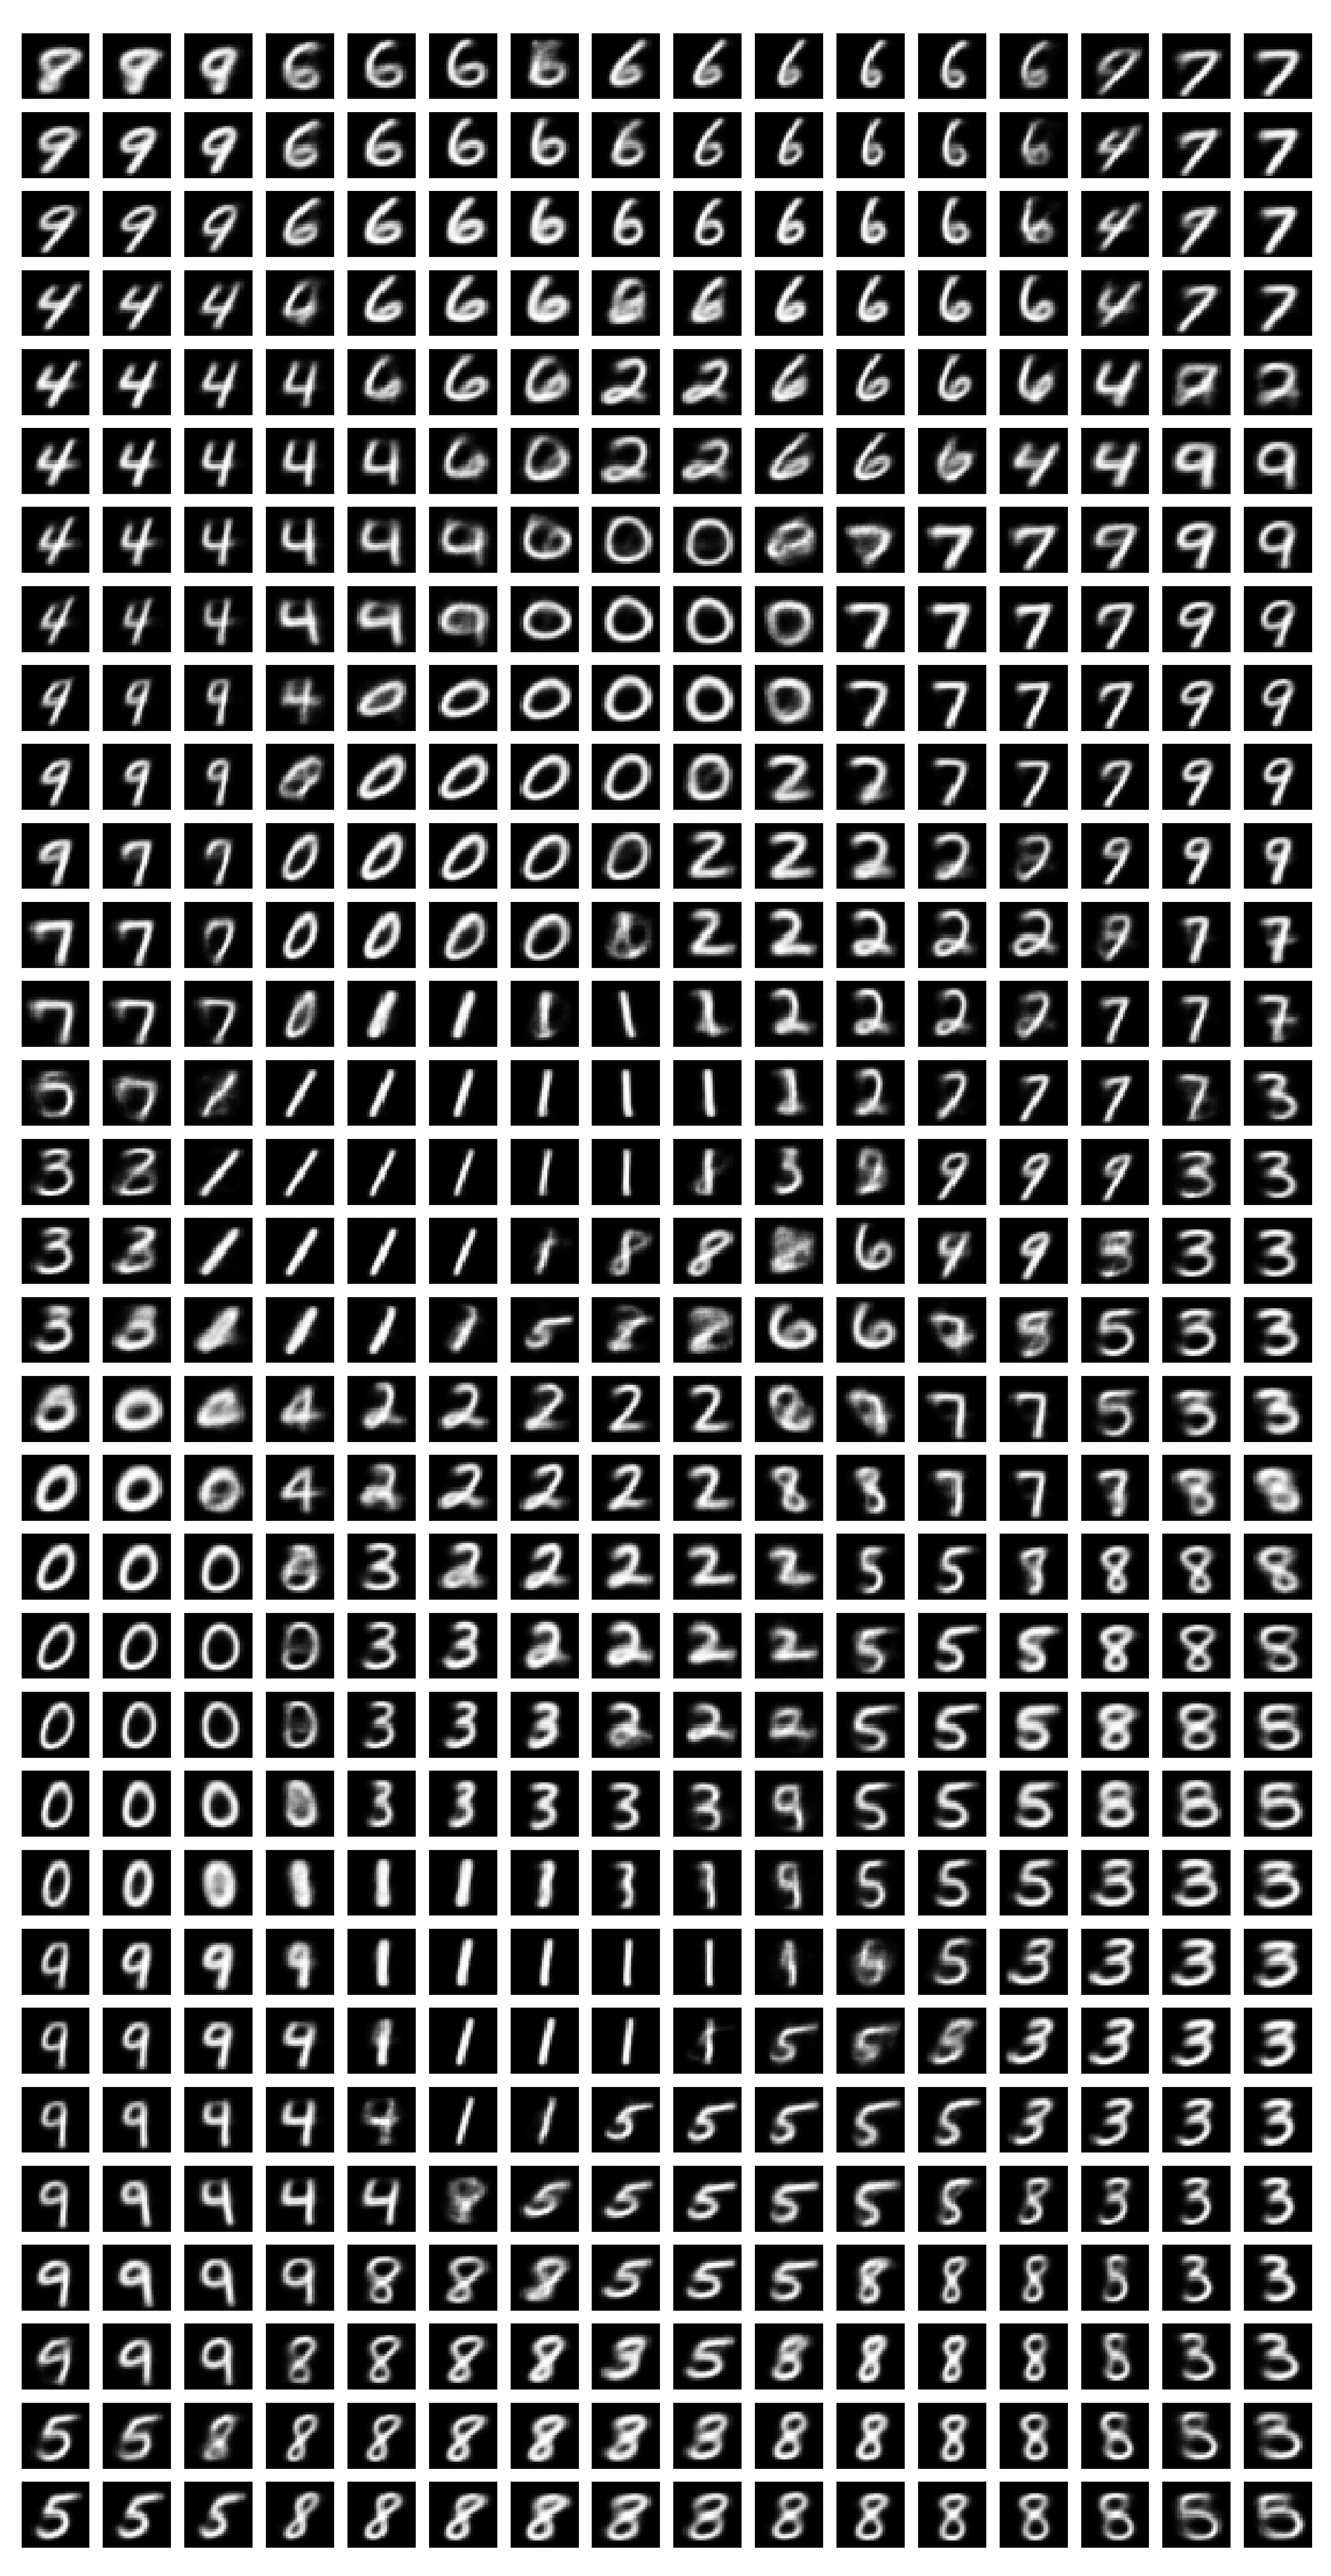
\includegraphics[height=0.8\textheight]{MNIST_SOM.pdf}
    \caption{Images generated from the SOM-VAE's latent space with 512 embeddings trained on MNIST. It yields an interpretable discrete two-dimensional representation of the data manifold in the higher-dimensional latent space.}
    \label{fig:MNIST_SOM}
\end{figure}

\begin{figure}[h]
    \centering
    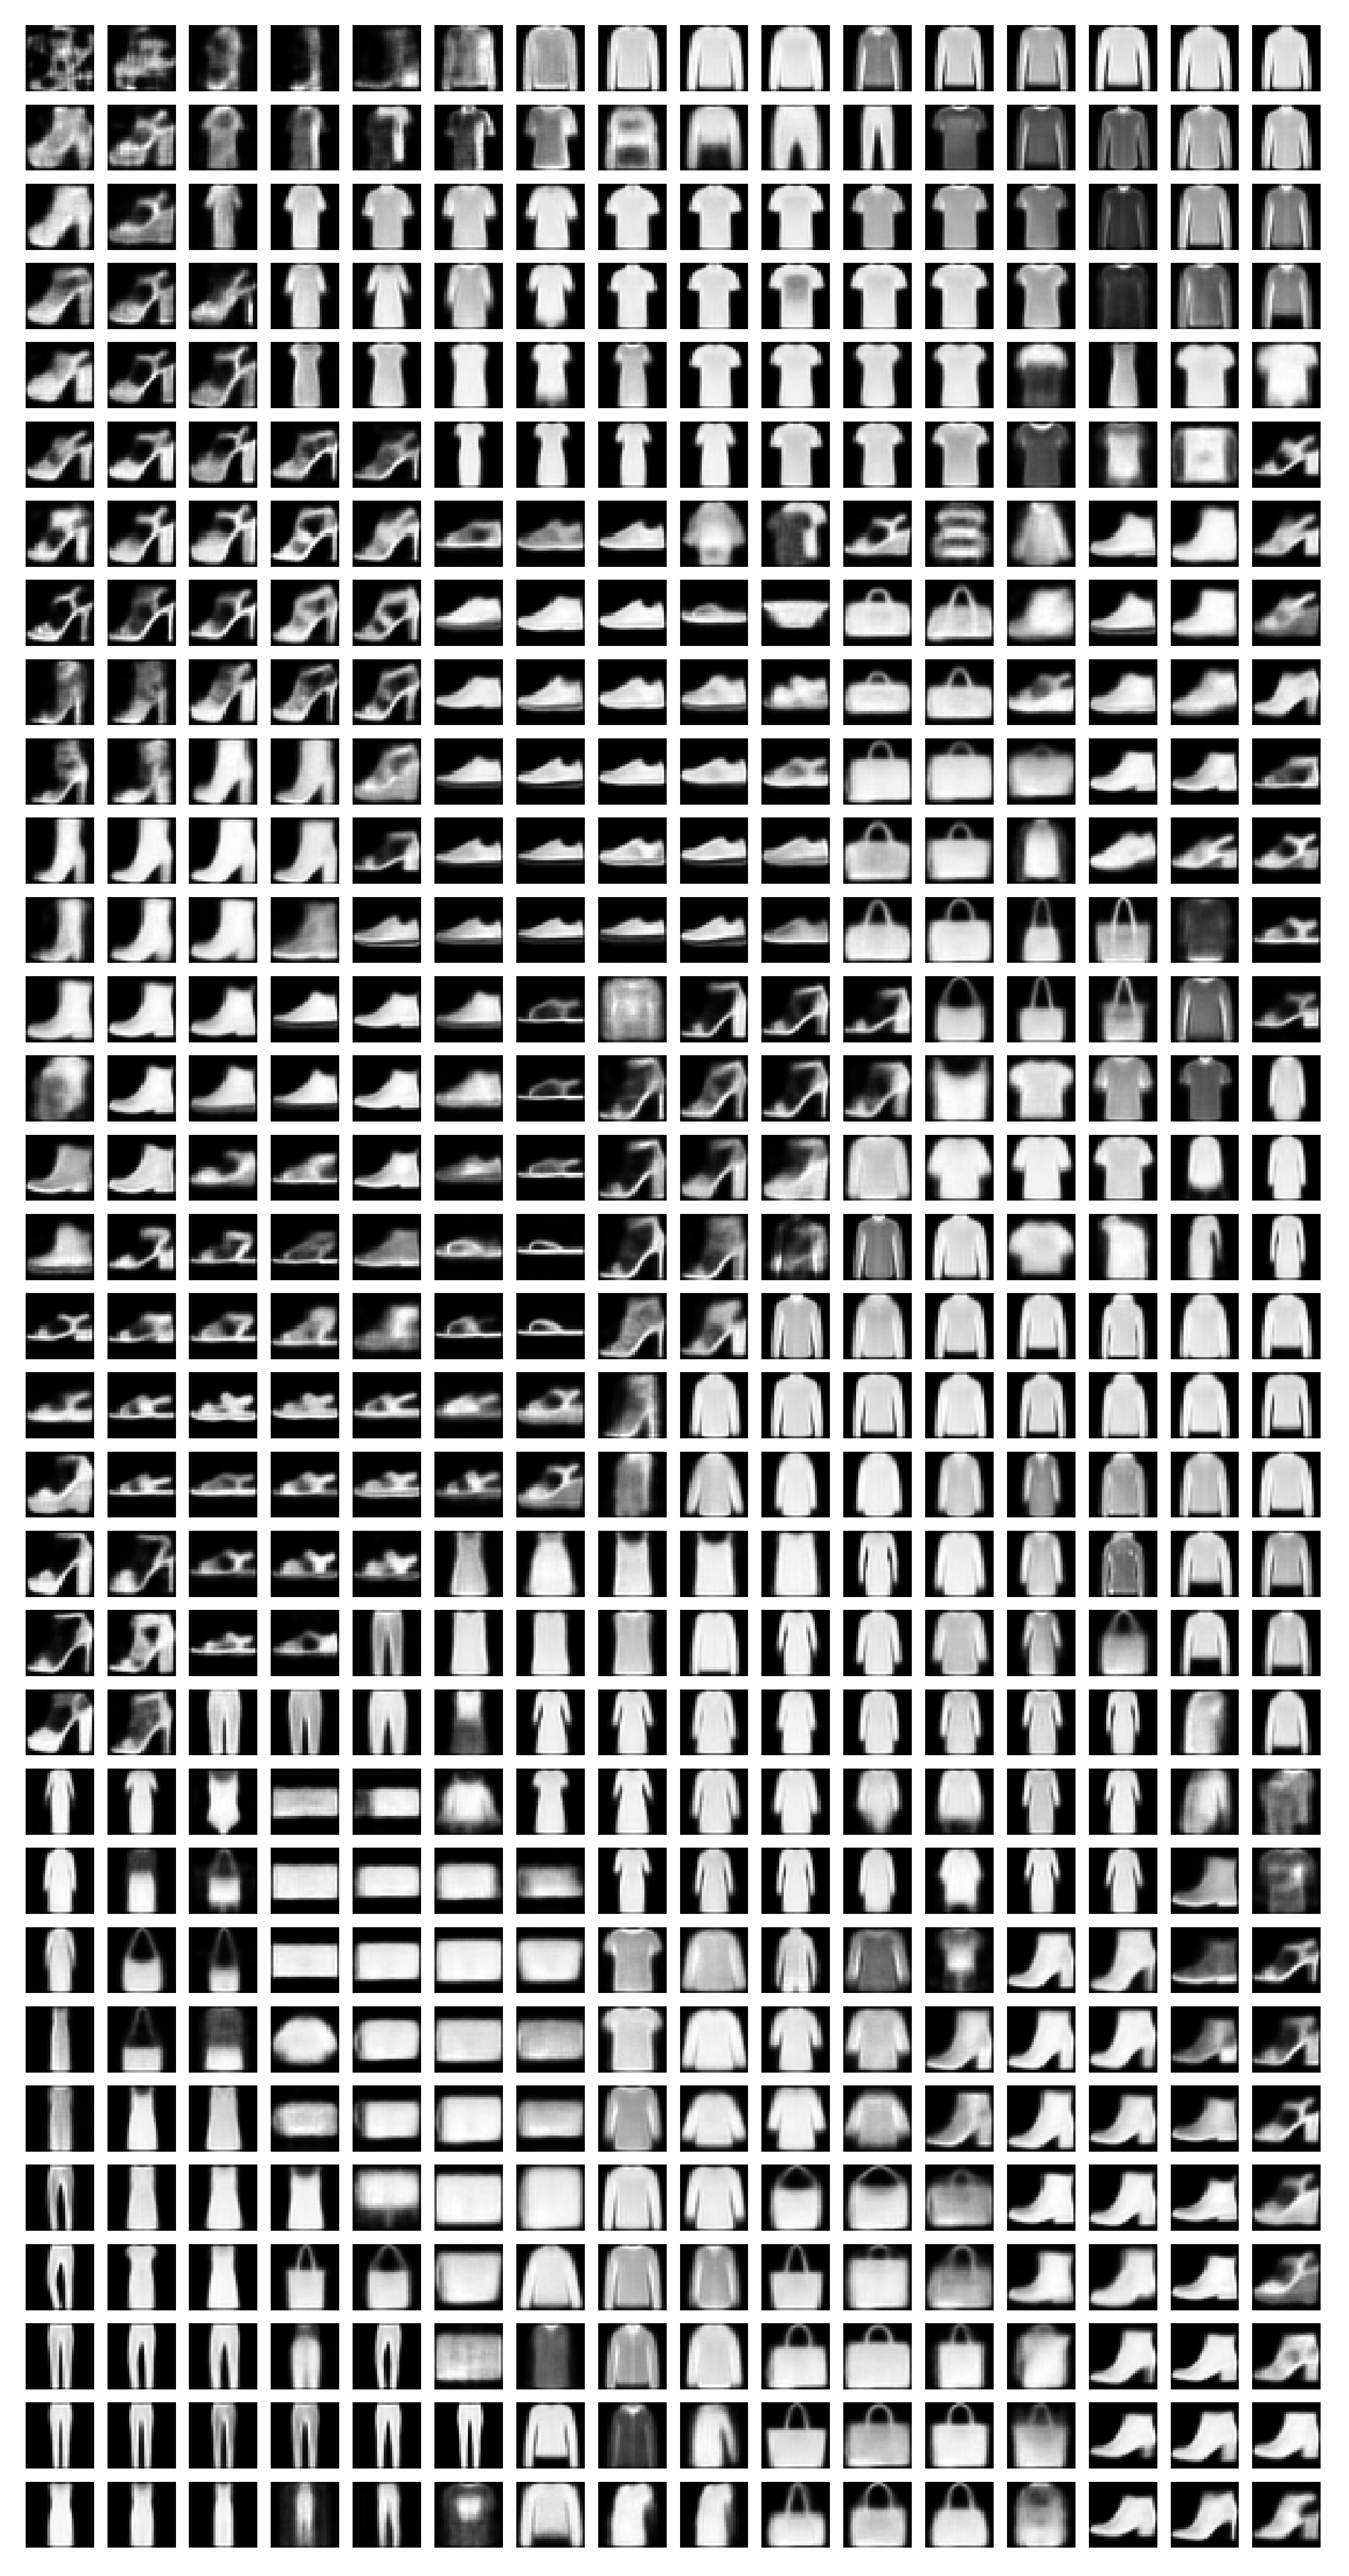
\includegraphics[height=0.8\textheight]{FMNIST_SOM.pdf}
    \caption{Images generated from the SOM-VAE's latent space with 512 embeddings trained on Fashion-MNIST. It yields an interpretable discrete two-dimensional representation of the data manifold in the higher-dimensional latent space.}
    \label{fig:FMNIST_SOM}
\end{figure}






	
\end{document}
\section{Related Work}

From the early inception of the \emph{k-means} algorithm for clustering \citep{Lloyd1982}, there has been much methodological improvement on this unsupervised task.
This includes methods that perform clustering in the latent space of (variational) autoencoders \citep{Aljalbout2018} or use a mixture of autoencoders for the clustering \citep{Zhang2017a, Locatello2018}.
The method most related to our work is the VQ-VAE \citep{Oord2017}, which can be seen as a special case of our framework (see above).
Its authors have put a stronger focus on the discrete representation as a form of compression instead of clustering.
Hence, our model and theirs differ in certain implementation considerations (see Sec.\ \ref{sec:non-differentiability}).
All these methods have in common that they only yield a single number as a cluster assignment and provide no interpretable structure of relationships between clusters.

The self-organizing map (SOM) \citep{Kohonen1998}, however, is an algorithm that provides such an interpretable structure.
It maps the data manifold to a lower-dimensional discrete space, which can be easily visualized in the 2D case.
It has been extended to model dynamical systems \citep{Barreto2004} and combined with probabilistic models for time series \citep{Sang2008}, although without using learned representations.
There are approaches to turn the SOM into a ``deeper'' model \citep{Dittenbach2000}, combine it with multi-layer perceptrons \citep{Furukawa2005} or with metric learning \citep{Ponski2014}.
However, it has (to the best of our knowledge) not been proposed to use SOMs in the latent space of (variational) autoencoders or any other form of unsupervised deep learning model.

Interpretable models for clustering and temporal predictions are especially crucial in fields where humans have to take responsibility for the model's predictions, such as in health care.
The prediction of a patient's future state is an important problem, particularly on the \emph{intensive care unit} (ICU) \citep{Harutyunyan2017, Badawi2018}.
Probabilistic models, such as Gaussian processes, have been successfully applied in this domain \citep{Colopy2016, Schulam2016}.
Recently, deep generative models have been proposed \citep{Hyland2017}, sometimes even in combination with probabilistic modeling \citep{Lim2018}.
To the best of our knowledge, SOMs have only been used to learn interpretable static representations of patients \citep{Tirunagari2015}, but not dynamic ones.
\section{Introduction}


Interpretable representation learning on time series is a seminal problem for uncovering the latent structure in complex systems, such as chaotic dynamical systems or medical time series.
In areas where humans have to make decisions based on large amounts of data, interpretability is fundamental to ease the human task.
Especially when decisions have to be made in a timely manner and rely on observing some chaotic external process over time, such as in finance or medicine, the need for intuitive interpretations is even stronger.
%Clinicians, for instance, might need to visualize and manually process the trajectory of a patient in order to decide on their treatment \citep{johnson16_machine_learning_decision}.
%They would benefit heavily from a representation learning model, in which those patient trajectories become intuitively understandable and relevant health features are salient.
%Since clinicians are already used to classifying patients into a finite set of discrete categories (e.g. using diagnosis codes), learned discrete health state representations would fit their intuition of a patient’s development.
%Clustering is a classical method for unsupervised discrete representation learning and is a natural solution for this problem at first sight.
However, many unsupervised methods, such as clustering, make misleading \emph{i.i.d.} assumptions about the data, neglecting their rich temporal structure and smooth behaviour over time.
This poses the need for a method of clustering, where the clusters assume a topological structure in a lower dimensional space, such that the representations of the time series retain their smoothness in that space.
In this work, we present a method with these properties.

We choose to employ deep neural networks, because they have a very successful tradition in representation learning \citep{Bengio2012}.
In recent years, they have increasingly been combined with generative modeling through the advent of generative adversarial networks (GANs) \citep{Goodfellow2014} and variational autoencoders (VAEs) \citep{Kingma2013}.
However, the representations learned by these models are often considered cryptic and do not offer the necessary interpretability \citep{Chen2016a}.
A lot of work has been done to improve them in this regard, in GANs \citep{Chen2016a} as well as VAEs \citep{Higgins2017, Esmaeili2018}.
Alas, these works have focused entirely on continuous representations, while discrete ones are still underexplored.

In order to define temporal smoothness in a discrete representation space, the space has to be equipped with a topological neighborhood relationship.
One type of representation space with such a structure is induced by the self-organizing map (SOM) \citep{Kohonen1998}.
The SOM allows to map states from an uninterpretable continuous space to a lower-dimensional space with a predefined topologically interpretable structure, such as an easily visualizable two-dimensional grid.
However, while yielding promising results in visualizing static state spaces, such as static patient states \citep{Tirunagari2015}, the classical SOM formulation does not offer a notion of time.
The time component can be incorporated using a probabilistic transition model, e.g.\ a Markov model, such that the representations of a single time point are enriched with information from the adjacent time points in the series.
It is therefore potentially fruitful to apply the approaches of probabilistic modeling alongside representation learning and discrete dimensionality reduction in an end-to-end model.

In this work, we propose a novel deep architecture that learns topologically interpretable discrete representations in a probabilistic fashion.
Moreover, we introduce a new method to overcome the non-differentiability in discrete representation learning architectures and develop a gradient-based version of the classical self-organizing map algorithm with improved performance.
We present extensive empirical evidence for the model's performance on synthetic and real world time series from benchmark data sets, a synthetic dynamical system with chaotic behavior and real world medical data.

Our main contributions are to

\begin{itemize}
	\item Devise a novel framework for interpretable discrete representation learning on time series.
	\item Show that the latent probabilistic model in the representation learning architecture improves clustering and interpretability of the representations on time series.
	\item Show superior clustering performance of the model on benchmark data and a real world medical data set, on which it also facilitates downstream tasks.
\end{itemize}
\FloatBarrier

\section{Probabilistic SOM-VAE}

Our proposed model combines ideas from self-organizing maps \citep{Kohonen1998}, variational autoencoders \citep{Kingma2013} and probabilistic models.
In the following, we will lay out the different components of the model and their interactions.


\subsection{Introducing Topological Structure in the Latent Space} \label{sec:SOM-VAE}

\begin{figure}
    \centering
    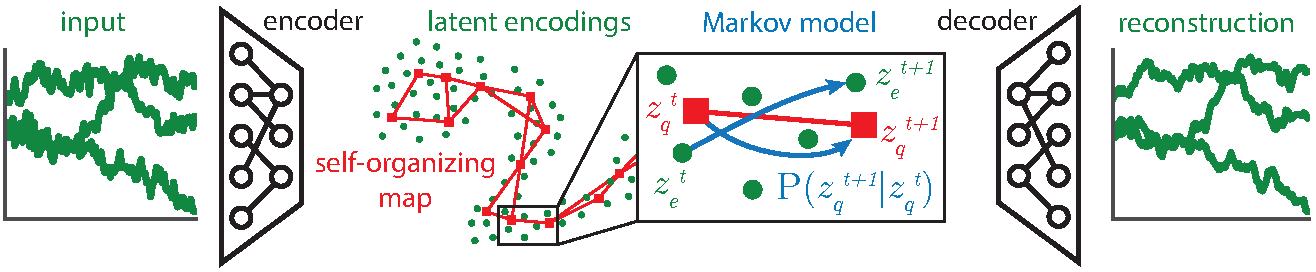
\includegraphics[width=\textwidth]{Overview_SOM-VAE.pdf}
    \caption{Schematic overview of our model architecture. Time series from the data space [green] are encoded by a neural network [black] time-point-wise into the latent space. The latent data manifold is approximated with a self-organizing map (SOM) [red]. In order to achieve a discrete representation, every latent data point ($z_e$) is mapped to its closest node in the SOM ($z_q$). A Markov transition model [blue] is learned to predict the next discrete representation ($z_q^{t+1}$) given the current one ($z_q^t$). The discrete representations can then be decoded by another neural network back into the original data space.}
    \label{fig:overview}
\end{figure}


A schematic overview of our proposed model is depicted in Figure \ref{fig:overview}.
An input $x \in \mathbb{R}^d$ is mapped to a latent encoding $z_e \in \mathbb{R}^m$ (usually $m < d$) by computing $z_e = f_{\theta}(x)$, where $f_{\theta}(\cdot)$ is parameterized by the encoder neural network.
The encoding is then assigned to an embedding $z_q \in \mathbb{R}^m$ in the dictionary of embeddings $E = \lbrace e_1, \dots, e_k \; \vert \; e_i \in \mathbb{R}^m \rbrace$ by sampling $z_q \sim p(z_q | z_e)$.
The form of this distribution is flexible and can be a design choice.
In order for the model to behave similarly to the original SOM algorithm (see below), in our experiments we choose the distribution to be categorical with probability mass 1 on the closest embedding to $z_e$, i.e.\ $p(z_q | z_e) = \mathds{1} \lbrack z_q = \argmin_{e \in E} \| z_e - e\|^2 \rbrack$, where $\mathds{1} \lbrack \cdot \rbrack$ is the indicator function.
A reconstruction $\hat{x}$ of the input can then be computed as $\hat{x} = g_{\phi}(z)$, where $g_{\phi}(\cdot)$ is parameterized by the decoder neural network.
Since the encodings and embeddings live in the same space, one can compute two different reconstructions, namely $\hat{x}_e = g_{\phi}(z_e)$ and $\hat{x}_q = g_{\phi}(z_q)$.

To achieve a topologically interpretable neighborhood structure, the embeddings are connected to form a self-organizing map.
A self-organizing map consists of $k$ nodes $V=\{v_1, \dots , v_k\}$, where every node corresponds to an embedding in the data space $e_v \in \mathbb{R}^d$ and a representation in a lower-dimensional discrete space $m_v \in M$, where usually $M \subset \mathbb{N}^2$.
During training on a data set $\mathcal{D} = \{x_1, \dots ,x_n\}$, a winner node $\tilde{v}$ is chosen for every point $x_i$ according to $\tilde{v} = \argmin_{v \in V} \| e_v - x_i \|^2$.
The embedding vector for every node $u \in V$ is then updated according to $e_u \leftarrow e_u + N(m_u,m_{\tilde{v}}) \eta (x_i - e_u)$, where $\eta$ is the learning rate and $N(m_u, m_{\tilde{v}})$ is a neighborhood function between the nodes defined on the representation space $M$.
There can be different design choices for $N(m_u, m_{\tilde{v}})$.
A more thorough review of the self-organizing map algorithm is deferred to the appendix (Sec.~\ref{sec:SOMs}).

We choose to use a two-dimensional SOM because it facilitates visualization similar to \citet{Tirunagari2015}.
Since we want the architecture to be trainable end-to-end, we cannot use the standard SOM training algorithm described above.
Instead, we devise a loss function term whose gradient corresponds to a weighted version of the original SOM update rule (see below).
We implement it in such a way that any time an embedding $e_{i,j}$ at position $(i,j)$ in the map gets updated, it also updates all the embeddings in its immediate neighborhood $N(e_{i,j})$.
The neighborhood is defined as $N(e_{i,j}) = \{ e_{i-1,j}, e_{i+1,j}, e_{i,j-1}, e_{i,j+1} \}$ for a two-dimensional map.

The loss function for a single input $x$ looks like
%
\begin{equation} \label{eq:L_somvae}
	\mathcal{L}_{\text{SOM-VAE}}(x, \hat{x}_q, \hat{x}_e) = \mathcal{L}_{\text{reconstruction}}(x, \hat{x}_q, \hat{x}_e) + \alpha \, \mathcal{L}_{\text{commitment}}(x) + \beta \, \mathcal{L}_{\text{SOM}}(x)
\end{equation}
%
where $x$, $z_e$, $z_q$, $\hat{x}_e$ and $\hat{x}_q$ are defined as above and $\alpha$ and $\beta$ are weighting hyperparameters.

Every term in this function is specifically designed to optimize a different model component.
The first term is the reconstruction loss $\mathcal{L}_{\text{reconstruction}}(x, \hat{x}_q, \hat{x}_e) = \| x - \hat{x}_q \|^2 + \| x - \hat{x}_e \|^2$.
The first subterm of this is the discrete reconstruction loss, which encourages the assigned SOM node $z_q(x)$ to be an informative representation of the input.
The second subterm encourages the encoding $z_e(x)$ to also be an informative representation.
This ensures that all parts of the model have a fully differentiable credit assignment path to the loss function, which facilitates training.
Note that the reconstruction loss corresponds to the evidence lower bound (ELBO) of the VAE part of our model \citep{Kingma2013}.
Since we assume a uniform prior over $z_q$, the KL-term in the ELBO is constant w.r.t.\ the parameters and can be ignored during optimization.

The term $\mathcal{L}_{\text{commitment}}$ encourages the encodings and assigned SOM nodes to be close to each other and is defined as $\mathcal{L}_{\text{commitment}}(x) = \| z_e(x) - z_q(x) \|^2$.
Closeness of encodings and embeddings should be expected to already follow from the $\mathcal{L}_{\text{reconstruction}}$ term in a fully differentiable architecture.
However, due to the non-differentiability of the embedding assignment in our model, the $\mathcal{L}_{\text{commitment}}$ term has to be explicitly added to the objective in order for the encoder to get gradient information about $z_q$.

The SOM loss $\mathcal{L}_{\text{SOM}}$ is defined as $\mathcal{L}_{\text{SOM}}(x) = \sum_{\tilde{e} \in N(z_q(x))} \| \tilde{e} - \text{sg}[z_e(x)] \|^2$, where $N(\cdot)$ is the set of neighbors in the discrete space as defined above and $\text{sg}[\cdot]$ is the gradient stopping operator that does not change the outputs during the forward pass, but sets the gradients to 0 during the backward pass.
It encourages the neighbors of the assigned SOM node $z_q$ to also be close to $z_e$, thus enabling the embeddings to exhibit a self-organizing map property, while stopping the gradients on $z_e$ such that the encoding is not pulled in the direction of the neighbors.
This term enforces a neighborhood relation between the discrete codes and encourages all SOM nodes to ultimately receive gradient information from the data.
The gradient stopping in this term is motivated by the observation that the data points themselves do not get moved in the direction of their assigned SOM node's neighbors in the original SOM algorithm either (see above).
We want to optimize the embeddings based on their neighbors, but not the respective encodings, since any single encoding should be as close as possible to its assigned embedding and not receive gradient information from any other embeddings that it is not assigned to.
Note that the gradient update of a specific SOM node in this formulation depends on its distance to the encoding, while the step size in the original SOM algorithm is constant.
It will be seen that this offers some benefits in terms of optimization and convergence (see Sec. \ref{sec:clustering_benchmark}).


\subsection{Overcoming the Non-Differentiability}\label{sec:non-differentiability}

The main challenge in optimizing our architecture is the non-differentiability of the discrete cluster assignment step.
Due to this, the gradients from the reconstruction loss cannot flow back into the encoder.
A model with a similar problem is the recently proposed vector-quantized VAE (VQ-VAE) \citep{Oord2017}.
It can be seen as being similar to a special case of our SOM-VAE model, where one sets $\beta = 0$, i.e. disables the SOM structure.

In order to mitigate the non-differentiability, the authors of the VQ-VAE propose to copy the gradients from $z_q$ to $z_e$.
They acknowledge that this is an \emph{ad hoc} approximation, but observed that it works well in their experiments.
Due to our smaller number of embeddings compared to the VQ-VAE setup, the average distance between an encoding and its closest embedding is much larger in our case.
The gradient copying (see above) thus ceases to be a feasible approximation, because the true gradients at points in the latent space which are farther apart will likely be very different.

In order to still overcome the non-differentiability issue, we propose to add the second reconstruction subterm to $\mathcal{L}_{\text{reconstruction}}$, where the reconstruction $\hat{x}_e$ is decoded directly from the encoding $z_e$.
This adds a fully differentiable credit assignment path from the loss to the encoder and encourages $z_e$ to also be an informative representation of the input, which is a desirable model feature.
Most importantly, it works well in practice (see Sec.\ \ref{sec:clustering_benchmark}).

Note that since $z_e$ is continuous and therefore much less constrained than $z_q$, this term is optimized easily and becomes small early in training.
After that, mostly the $z_q$-term contributes to $\mathcal{L}_{\text{reconstruction}}$.
One could therefore view the $z_e$-term as an initial encouragement to place the data encodings at sensible positions in the latent space, after which the actual clustering task dominates the training objective.



\subsection{Encouraging Smoothness over Time}\label{sec:probabilistic_model}

Our ultimate goal is to predict the development of time series in an interpretable way.
This means that not only the state representations should be interpretable, but so should be the prediction as well.
To this end, we use a temporal probabilistic model.

Learning a probabilistic model in a high-dimensional continuous space can be challenging.
Thus, we exploit the low-dimensional discrete space induced by our SOM to learn a temporal model.
For that, we define a system state as the assigned node in the SOM and then learn a Markov model for the transitions between those states.
The model is learned jointly with the SOM-VAE, where the loss function becomes
%
\begin{equation}\label{eq:L_prob}
    \mathcal{L}(x^{t-1}, x^t, \hat{x}_q^t, \hat{x}_e^t) = \mathcal{L}_{\text{SOM-VAE}}(x^t, \hat{x}_q^t, \hat{x}_e^t) + \gamma \, \mathcal{L}_{\text{transitions}}(x^{t-1}, x^t) + \tau \, \mathcal{L}_{\text{smoothness}}(x^{t-1}, x^t)
\end{equation}
%
with weighting hyperparameters $\gamma$ and $\tau$.

The term $\mathcal{L}_{\text{transitions}}$ encourages the probabilities of actually observed transitions to be high.
It is defined as $\mathcal{L}_{\text{transitions}}(x^{t-1}, x^t) = - \log P_{M} (z_q(x^{t-1}) \rightarrow z_q(x^t))$, with $P_{M} (z_q(x^{t-1}) \rightarrow z_q(x^t))$ being the probability of a transition from state $z_q(x^{t-1})$ to state $z_q(x^t)$ in the Markov model.

The term $\mathcal{L}_{\text{smoothness}}$ encourages the probabilities for transitions to nodes that are far away from the current data point to be low or respectively the nodes with high transition probabilities to be proximal.
It achieves this by taking large values only for transitions to far away nodes that have a high probability under the model.
It is defined as $\mathcal{L}_{\text{smoothness}}(x^{t-1}, x^t) = \mathbb{E}_{P_{M} \left( z_q(x^{t-1}) \rightarrow \tilde{e} \right) } \left[ \| \tilde{e} - z_e(x^t) \|^2 \right]$.
The probabilistic model can inform the evolution of the SOM through this term which encodes our prior belief that transitions in natural data happen smoothly and that future time points will therefore mostly be found in the neighborhood of previous ones.
In a setting where the data measurements are noisy, this improves the clustering by acting as a temporal smoother.


\section{Experiments}\label{sec:experiments}

We performed experiments on MNIST handwritten digits \citep{LeCun1998}, Fashion-MNIST images of clothing \citep{Xiao2017}, synthetic time series of linear interpolations of those images, time series from a chaotic dynamical system and real world medical data from the \emph{eICU Collaborative Research Database} \citep{Goldberger2000}.
If not otherwise noted, we use the same architecture for all experiments, sometimes including the latent probabilistic model (\emph{SOM-VAE\_prob}) and sometimes excluding it (\emph{SOM-VAE}).
For model implementation details, we refer to the appendix (Sec.~\ref{sec:implementation})\footnote{Our code is available at \url{https://github.com/ratschlab/SOM-VAE}.}.

We found that our method achieves a superior clustering performance compared to other methods.
We also show that we can learn a temporal probabilistic model concurrently with the clustering, which is on par with the maximum likelihood solution, while improving the clustering performance.
Moreover, we can learn interpretable state representations of a chaotic dynamical system and discover patterns in real medical data.


\subsection{Clustering on MNIST and Fashion-MNIST}\label{sec:clustering_benchmark}

In order to test the clustering component of the SOM-VAE, we performed experiments on MNIST and Fashion-MNIST.
We compare our model (including different adjustments to the loss function) against k-means \citep{Lloyd1982} (\texttt{sklearn}-package \citep{Pedregosa2011}), the VQ-VAE \citep{Oord2017}, a standard implementation of a SOM (\texttt{minisom}-package \citep{Vettigli2017}) and our version of a GB-SOM (gradient-based SOM), which is a SOM-VAE where the encoder and decoder are set to be identity functions.
The k-means algorithm was initialized using k-means++ \citep{Arthur2007-rk}.
To ensure comparability of the performance measures, we used the same number of clusters (i.e.\ the same $k$) for all the methods.

The results of the experiment in terms of purity and normalized mutual information (NMI) are shown in Table~\ref{tab:performance}.
The SOM-VAE outperforms the other methods w.r.t.\ the clustering performance measures.
It should be noted here that while k-means is a strong baseline, it is not density matching, i.e.\ the density of cluster centers is not proportional to the density of data points.
Hence, the representation of data in a space induced by the k-means clusters can be misleading.

As argued in the appendix (Sec.~\ref{sec:clustering_performance}), NMI is a more balanced measure for clustering performance than purity.
If one uses 512 embeddings in the SOM, one gets a lower NMI due to the penalty term for the number of clusters, but it yields an interpretable two-dimensional representation of the manifolds of MNIST (Fig.~\ref{fig:MNIST_SOM_selection}, Supp.~Fig.~\ref{fig:MNIST_SOM}) and Fashion-MNIST (Supp.\ Fig.~\ref{fig:FMNIST_SOM}).

\begin{figure}
    \centering
    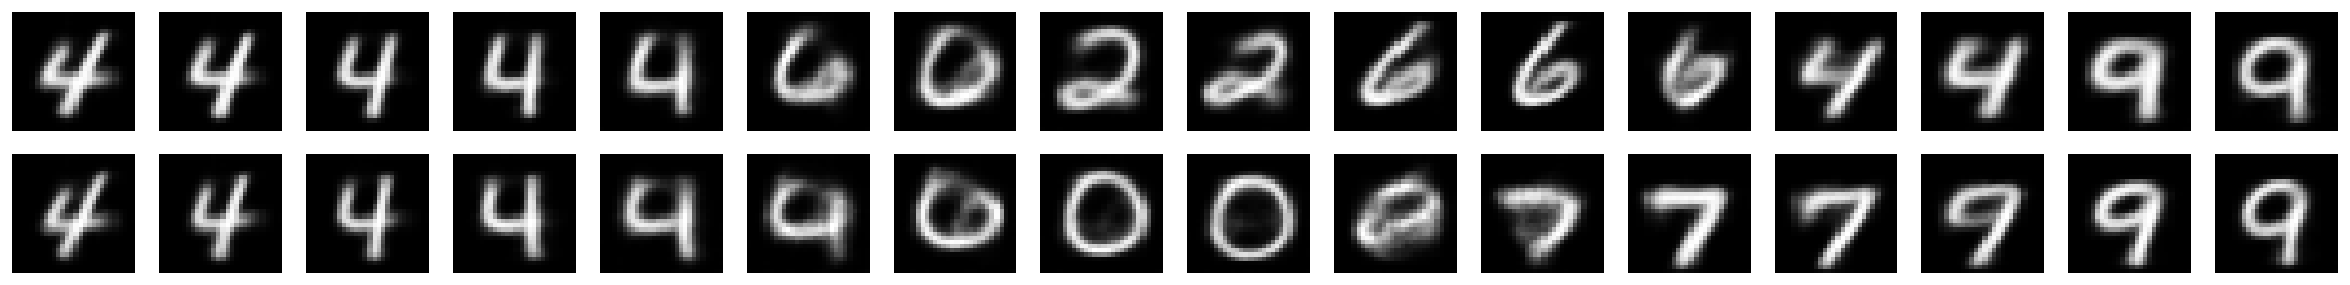
\includegraphics[width=0.9\textwidth]{MNIST_somvae_selection.pdf}
    \caption{Images generated from a section of the SOM-VAE's latent space with 512 embeddings trained on MNIST. It yields a discrete two-dimensional representation of the data manifold in the higher-dimensional latent space.}
    \label{fig:MNIST_SOM_selection}
\end{figure}

The experiment shows that the SOM in our architecture improves the clustering (SOM-VAE vs.\ VQ-VAE) and that the VAE does so as well (SOM-VAE vs.\ GB-SOM).
Both parts of the model therefore seem to be beneficial for our task.
It also becomes apparent that our reconstruction loss term on $z_e$ works better in practice than the gradient copying trick from the VQ-VAE (SOM-VAE vs.\ gradcopy), due to the reasons described in Section~\ref{sec:non-differentiability}.
If one removes the $z_e$ reconstruction loss and does not copy the gradients, the encoder network does not receive any gradient information any more and the learning fails completely (no\_grads).
Another interesting observation is that stochastically optimizing our SOM loss using Adam \citep{Kingma2015} seems to discover a more performant solution than the classical SOM algorithm (GB-SOM vs.\ minisom).
This could be due to the dependency of the step size on the distance between embeddings and encodings, as described in Section~\ref{sec:SOM-VAE}.
Since k-means seems to be the strongest competitor, we are including it as a reference baseline in the following experiments as well.


\begin{table}
    \centering
    \caption{Performance comparison of our method and some baselines in terms of purity and normalized mutual information on different benchmark data sets. The methods marked with an asterisk are variants of our proposed method. The values are the means of 10 runs and the respective standard errors. Each method was used to fit 16 embeddings/clusters.}
    \begin{tabular}{lrrrr}
        \toprule
         & \multicolumn{2}{c}{MNIST} & \multicolumn{2}{c}{Fashion-MNIST} \\
        \cmidrule(rl){2-3}
        \cmidrule(rl){4-5}
        Method & \multicolumn{1}{c}{Purity} & \multicolumn{1}{c}{NMI} & \multicolumn{1}{c}{Purity} & \multicolumn{1}{c}{NMI} \\
         \midrule
         k-means & 0.690 $\pm$ 0.000 & 0.541 $\pm$ 0.001 & 0.654 $\pm$ 0.001 & 0.545 $\pm$ 0.000 \\
         minisom & 0.406 $\pm$ 0.006 & 0.342 $\pm$ 0.012 & 0.413 $\pm$ 0.006 & 0.475 $\pm$ 0.002 \\
         GB-SOM & 0.653 $\pm$ 0.007 & 0.519 $\pm$ 0.005 & 0.606 $\pm$ 0.006 & 0.514 $\pm$ 0.004 \\
         VQ-VAE & 0.538 $\pm$ 0.067 & 0.409 $\pm$ 0.065 & 0.611 $\pm$ 0.006 & 0.517 $\pm$ 0.002 \\
         no\_grads* & 0.114 $\pm$ 0.000 & 0.001 $\pm$ 0.000 & 0.110 $\pm$ 0.009 & 0.018 $\pm$ 0.016 \\
         gradcopy* & 0.583 $\pm$ 0.004 & 0.436 $\pm$ 0.004 & 0.556 $\pm$ 0.008 & 0.444 $\pm$ 0.005 \\
         SOM-VAE* & \textbf{0.731 $\pm$ 0.004} & \textbf{0.594 $\pm$ 0.004} & \textbf{0.678 $\pm$ 0.005} & \textbf{0.590 $\pm$ 0.003} \\
         \bottomrule
    \end{tabular}
    \label{tab:performance}
\end{table}

\FloatBarrier

\subsection{Markov transition model on the discrete representations}

In order to test the probabilistic model in our architecture and its effect on the clustering, we generated synthetic time series data sets of (Fashion-)MNIST images being linearly interpolated into each other.
Each time series consists of 64 frames, starting with one image from \mbox{(Fashion-)MNIST} and smoothly changing sequentially into four other images over the length of the time course.

After training the model on these data, we constructed the maximum likelihood estimate (MLE) for the Markov model's transition matrix by fixing all the weights in the SOM-VAE and making another pass over the training set, counting all the observed transitions.
This MLE transition matrix reaches a negative log likelihood of $0.24$, while our transition matrix, which is learned concurrently with the architecture, yields $0.25$.
Our model is therefore on par with the MLE solution.

Comparing these results with the clustering performance on the standard MNIST and Fashion-MNIST test sets, we observe that the performance in terms of NMI is not impaired by the inclusion of the probabilistic model into the architecture (Tab.~\ref{tab:performance_prob}).
On the contrary, the probabilistic model even slightly increases the performance on Fashion-MNIST.
Note that we are using 64 embeddings in this experiment instead of 16, leading to a higher clustering performance in terms of purity, but a slightly lower performance in terms of NMI compared to Table~\ref{tab:performance}.
This shows again that the measure of purity has to be interpreted with care when comparing different experimental setups and that therefore the normalized mutual information should be preferred to make quantitative arguments.

This experiment shows that we can indeed fit a valid probabilistic transition model concurrently with the SOM-VAE training, while at the same time not hurting the clustering performance.
It also shows that for certain types of data the clustering performance can even be improved by the probabilistic model (see Sec.~\ref{sec:probabilistic_model}).

\begin{table}
    \centering
    \caption{Performance comparison of the SOM-VAE with and without latent Markov model (SOM-VAE-prob) against k-means in terms of purity and normalized mutual information on different benchmark data sets. The values are the means of 10 runs and the respective standard errors. Each method is used to fit 64 embeddings/clusters.}
    \begin{tabular}{lrrrr}
        \toprule
         & \multicolumn{2}{c}{MNIST} & \multicolumn{2}{c}{Fashion-MNIST} \\
        \cmidrule(rl){2-3}
        \cmidrule(rl){4-5}
        Method & \multicolumn{1}{c}{Purity} & \multicolumn{1}{c}{NMI} & \multicolumn{1}{c}{Purity} & \multicolumn{1}{c}{NMI} \\
         \midrule
         k-means & 0.791 $\pm$ 0.005 & 0.537 $\pm$ 0.001 & 0.703 $\pm$ 0.002 & 0.492 $\pm$ 0.001 \\
         SOM-VAE & \textbf{0.868 $\pm$ 0.003} & \textbf{0.595 $\pm$ 0.002} & \textbf{0.739 $\pm$ 0.002} & 0.520 $\pm$ 0.002 \\
         SOM-VAE-prob & 0.858 $\pm$ 0.004 & \textbf{0.596 $\pm$ 0.001} & 0.724 $\pm$ 0.003 & \textbf{0.525 $\pm$ 0.002} \\
         \bottomrule
    \end{tabular}
    \label{tab:performance_prob}
\end{table}


\subsection{Interpretable representations of chaotic time series} \label{sec:lorenz}

In order to assess whether our model can learn an interpretable representation of more realistic chaotic time series, we train it on synthetic trajectories simulated from the famous \emph{Lorenz system} \citep{Lorenz1963}.
The Lorenz system is a good example for this assessment, since it offers two well defined macro-states (given by the attractor basins) which are occluded by some chaotic noise in the form of periodic fluctuations around the attractors.
A good interpretable representation should therefore learn to largely ignore the noise and model the changes between attractor basins.
For a review of the Lorenz system and details about the simulations and the performance measure, we refer to the appendix (Sec.~\ref{sec:lorenz_appendix}).

In order to compare the interpretability of the learned representations, we computed entropy distributions over simulated subtrajectories in the real system space, the attractor assignment space and the representation spaces for k-means and our model.
The computed entropy distributions over all subtrajectories in the test set are depicted in Figure~\ref{fig:lorenz}. 

\begin{figure}[h!]
    \centering
    \begin{subfigure}[t]{0.15\textwidth}
\centering
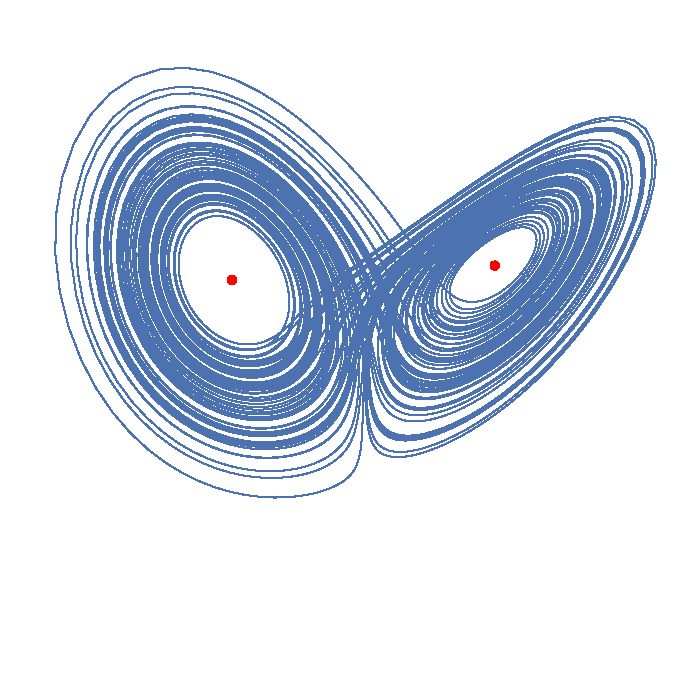
\includegraphics[scale=0.19]{lorenz/lorenz_attractor.pdf}
\subcaption{Lorenz attractor}
\end{subfigure}
    \begin{subfigure}[t]{0.15\textwidth}
\centering
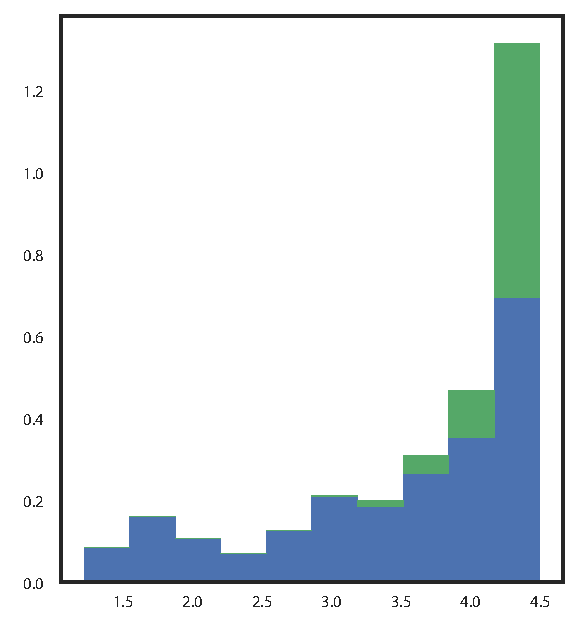
\includegraphics[scale=0.22]{lorenz/real_space.pdf}
\subcaption{Real space}
\label{fig:lorenz_real}
\end{subfigure}
    \begin{subfigure}[t]{0.15\textwidth}
\centering
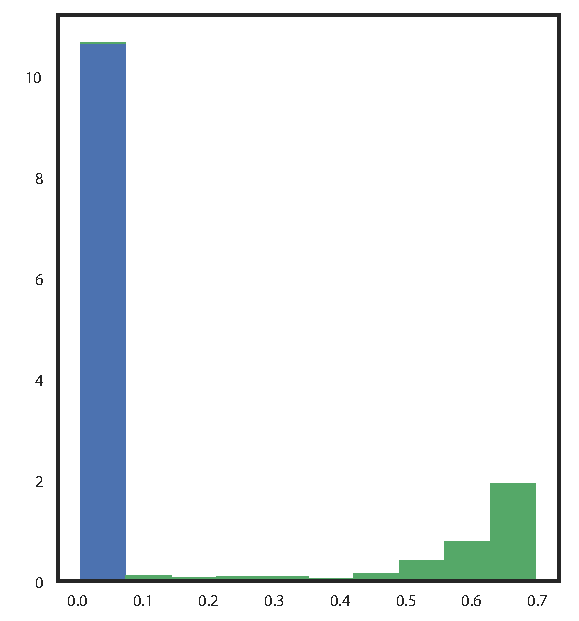
\includegraphics[scale=0.22]{lorenz/attractor_assignment.pdf}
\subcaption{Attractor assigment}
\label{fig:lorenz_assignment}
\end{subfigure}
    \begin{subfigure}[t]{0.15\textwidth}
\centering
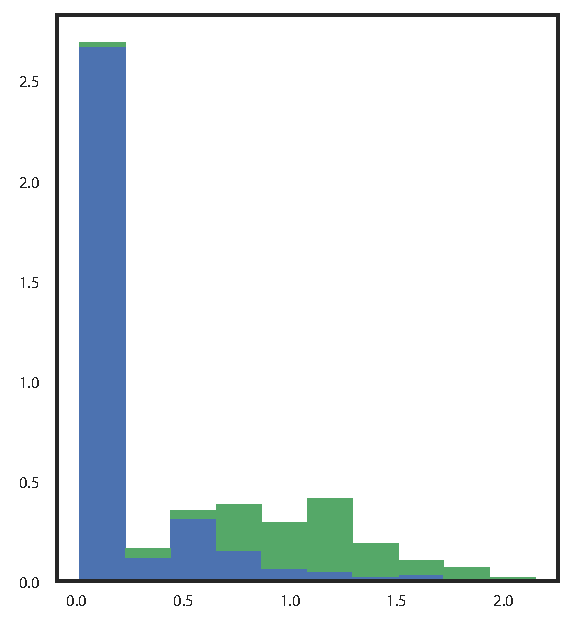
\includegraphics[scale=0.22]{lorenz/SOM_VAE.pdf}
\subcaption{SOM-VAE}
\label{fig:lorenz_somvae}
\end{subfigure}
    \begin{subfigure}[t]{0.15\textwidth}
\centering
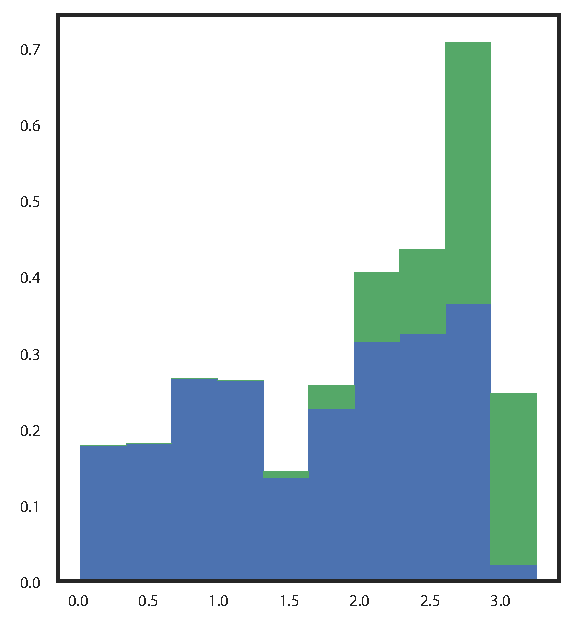
\includegraphics[scale=0.22]{lorenz/k_means.pdf}
\subcaption{k-means}
\label{fig:lorenz_kmeans}
\end{subfigure}
    \begin{subfigure}[t]{0.15\textwidth}
\centering
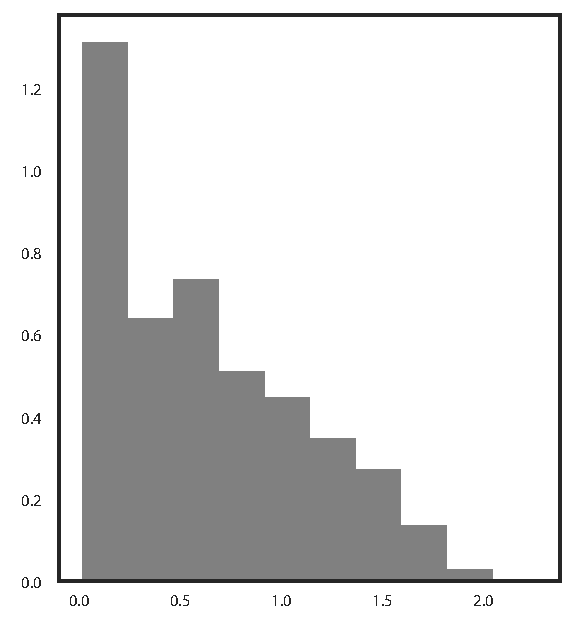
\includegraphics[scale=0.22]{lorenz/simulated.pdf}
\subcaption{Simulated trajectories}
\label{fig:lorenz_simulated}
\end{subfigure}

    \caption{Histograms of entropy distributions (entropy on the x-axes) over all Lorenz attractor subtrajectories [a] of 100 time steps length in our test set. Subtrajectories without a change in attractor basin are colored in blue, the ones where a change has taken place in green.}
    \label{fig:lorenz}
\end{figure}

The experiment shows that the SOM-VAE representations (Fig.~\ref{fig:lorenz_somvae}) are much closer in entropy to the ground-truth attractor basin assignments (Fig. \ref{fig:lorenz_assignment}) than the k-means representations (Fig. \ref{fig:lorenz_kmeans}).
For most of the subtrajectories without attractor basin change they assign a very low entropy, effectively ignoring the noise, while the k-means representations partially assign very high entropies to those trajectories.
In total, the k-means representations' entropy distribution is similar to the entropy distribution in the noisy system space (Fig.~\ref{fig:lorenz_real}).
The representations learned by the SOM-VAE are therefore more interpretable than the k-means representations with regard to this interpretability measure.
As could be expected from these figures, the SOM-VAE representation is also superior to the k-means one in terms of purity with respect to the attractor assignment ($0.979$ vs.\ $0.956$) as well as NMI ($0.577$ vs.\ $0.249$).

Finally, we use the learned probabilistic model on our SOM-VAE representations to sample new latent system trajectories and compute their entropies.
The distribution looks qualitatively similar to the one over real trajectories (Fig.\ \ref{fig:lorenz}), but our model slightly overestimates the attractor basin change probabilities, leading to a heavier tail of the distribution.

\FloatBarrier

\subsection{Learning representations of real medical time series}


In order to demonstrate interpretable representation learning on a complex real world task, we trained our model on vital sign time series measurements of intensive care unit (ICU) patients.
We analyze the performance of the resulting clustering w.r.t.\ the patients' future physiology states in Table \ref{tab:dynamic_performance_ICU}.
This can be seen as a way to assess the representations' informativeness for a downstream prediction task.
For details regarding the data selection and processing, we refer to the appendix (Sec.\ \ref{sec:ICU_appendix}).

\begin{table}
    \centering
    \caption{Performance comparison of our method with and without probabilistic model (SOM-VAE-prob and SOM-VAE) against k-means in terms of normalized mutual information on a challenging unsupervised prediction task on real eICU data. The dynamic endpoints are the maximum of the physiology score within the next 6, 12 or 24 hours (\emph{physiology\_6\_hours}, \emph{physiology\_12\_hours}, \emph{physiology\_24\_hours}). The values are the means of 10 runs and the respective standard errors. Each method is used to fit 64 embeddings/clusters.}
    \begin{tabular}{lrrr}
        \toprule
        Method & \multicolumn{1}{c}{physiology\_6\_hours} & \multicolumn{1}{c}{physiology\_12\_hours} & \multicolumn{1}{c}{physiology\_24\_hours} \\
         \midrule
         k-means & 0.0411 $\pm$ 0.0007 & 0.0384 $\pm$ 0.0006 & 0.0366 $\pm$ 0.0005 \\
         SOM-VAE & 0.0407 $\pm$ 0.0005 & 0.0376 $\pm$ 0.0004 & 0.0354 $\pm$ 0.0004 \\
         SOM-VAE-prob & \textbf{0.0474 $\pm$ 0.0006} & \textbf{0.0444 $\pm$ 0.0006} & \textbf{0.0421 $\pm$ 0.0005} \\
         \bottomrule
    \end{tabular}
    \label{tab:dynamic_performance_ICU}
\end{table}

Our full model (including the latent Markov model) performs best on the given tasks, i.e.\ better than k-means and also better than the SOM-VAE without probabilistic model.
This could be due to the noisiness of the medical data and the probabilistic model's smoothing tendency (see Sec.~\ref{sec:probabilistic_model}).

In order to qualitatively assess the interpretability of the probabilistic SOM-VAE, we analyzed the average future physiology score per cluster (Fig.~\ref{fig:heatmaps}).
Our model exhibits clusters where higher scores are enriched compared to the background level.
Moreover, these clusters form compact structures, facilitating interpretability.
We do not observe such interpretable structures in the other methods. For full results on acute physiology scores, an analogue experiment showing the 
future mortality risk associated with different regions of the map, and an analysis of enrichment for
particular physiological abnormalities, we refer to the appendix (Sec.\ \ref{subsec:detailed_icu}). 

As an illustrative example for data visualization using our method, we show the trajectories of two patients that start in the same state (Fig.~\ref{fig:patient_trajectories}).
The trajectories are plotted in the representation space of the probabilistic SOM-VAE and should thus be compared to the visualization in Figure~\ref{fig:ICU_representations}.
One patient (\emph{green}) stays in the regions of the map with low average physiology score and eventually gets discharged from the hospital healthily.
The other one (\emph{red}) moves into map regions with high average physiology score and ultimately dies.
Such knowledge could be helpful for doctors, who could determine the risk of a patient for certain deterioration scenarios from a glance at their trajectory in the SOM-VAE representation.

\begin{figure}
\centering
\begin{subfigure}[t]{0.22\textwidth}
\centering
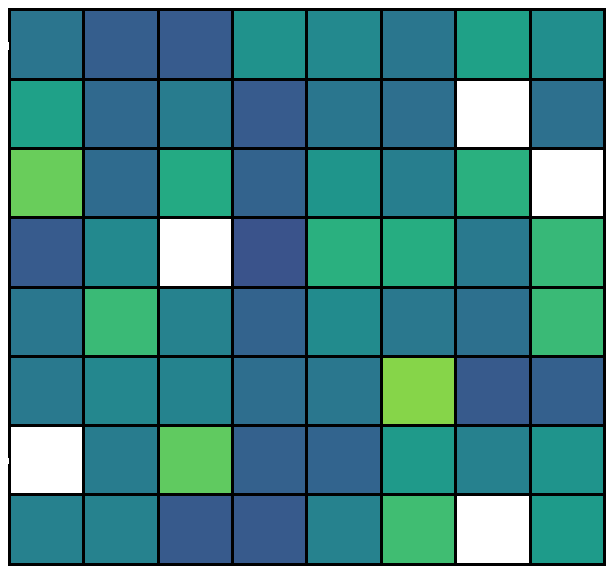
\includegraphics[scale=0.25]{k_means_full_score_24_enrichment_heatmap.pdf}
\subcaption{k-means}
\end{subfigure}
\begin{subfigure}[t]{0.22\textwidth}
\centering
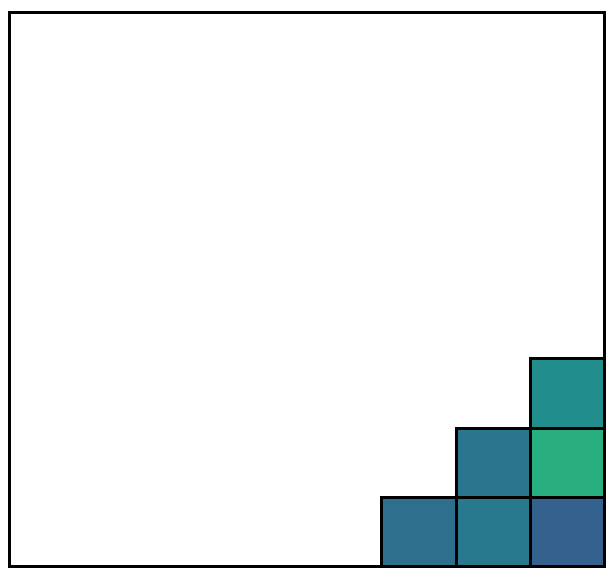
\includegraphics[scale=0.25]{vqvae_full_score_24_enrichment_heatmap.pdf}
\subcaption{VQ-VAE}
\end{subfigure}
\begin{subfigure}[t]{0.22\textwidth}
\centering
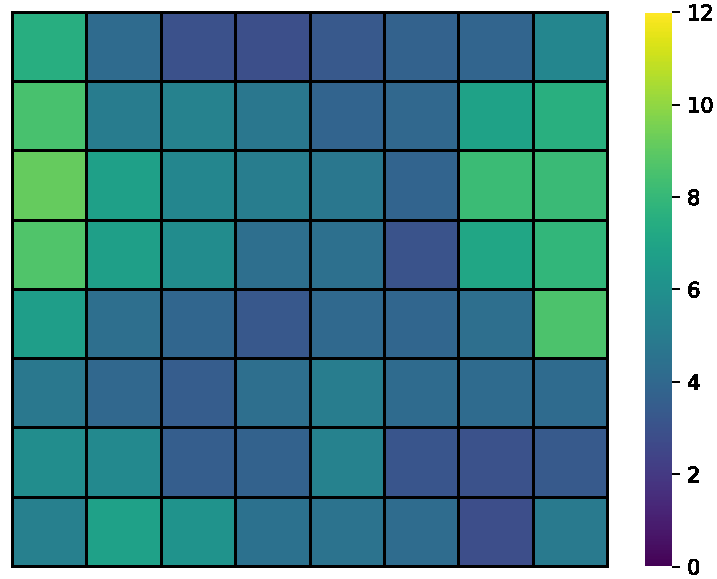
\includegraphics[scale=0.25]{somvae_prob_full_score_24_enrichment_heatmap.pdf}
\subcaption{SOM-VAE-prob}
\label{fig:ICU_representations}
\end{subfigure}
\begin{subfigure}[t]{0.22\textwidth}
\centering
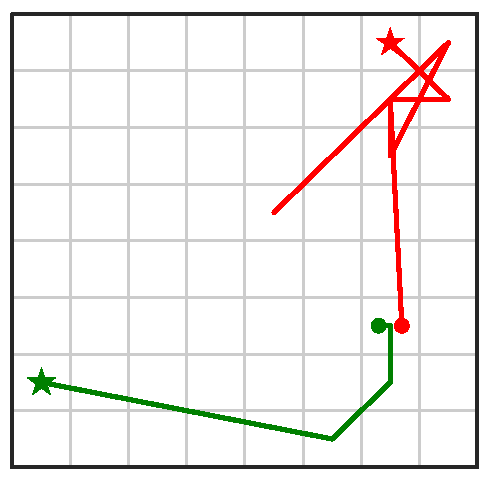
\includegraphics[scale=0.31]{patient_trajectory_example.pdf}
\subcaption{Patient trajectories}
\label{fig:patient_trajectories}
\end{subfigure}
\caption{Comparison of the patient state representations learned by different models. The clusters are colored by degree of patient abnormality as measured by a variant of the APACHE physiology score (more yellow means ``less healthy'').
White squares correspond to unused clusters, i.e.\ clusters that contain less than 0.1 percent of the data points.
Subfigure (d) shows two patient trajectories in the SOM-VAE-prob representation over their respective whole stays in the ICU.
The dots mark the ICU admission, the stars the discharge from the ICU (cured [green] or dead [red]).
It can be seen that our model is the only one that learns a topologically interpretable structure.
}
\label{fig:heatmaps}
\end{figure}



\usepackage[utf8]{inputenc} % allow utf-8 input
\usepackage[T1]{fontenc}    % use 8-bit T1 fonts
%\usepackage{hyperref}       % hyperlinks
%\usepackage{url}            % simple URL typesetting
\usepackage{booktabs}       % professional-quality tables
\usepackage{amsfonts}       % blackboard math symbols
\usepackage{amsmath}
\usepackage{dsfont}
\usepackage{nicefrac}       % compact symbols for 1/2, etc.
\usepackage{microtype}      % microtypography
\usepackage{siunitx}
\usepackage{color}
\usepackage{graphicx}
\usepackage{tabularx}
\usepackage{caption}
\usepackage{subcaption}
\usepackage[english]{babel}
\usepackage{placeins}
\usepackage{algorithm}
\usepackage{algorithmicx}
\usepackage{algpseudocode}
\usepackage{url}

% For commenting the draft:
\usepackage{lineno}
%\linenumbers


\usepackage[letterpaper, total={6in, 9in}]{geometry}

%\usepackage[square,sort,comma,numbers]{natbib}
%\usepackage{natbib}


%\renewcommand\Affilfont{\footnotesize}

\bibliographystyle{plainnat}

\DeclareMathOperator*{\argmin}{arg\,min}

\graphicspath{{./figures/}}

\newcommand{\fix}{\marginpar{FIX}}
\newcommand{\new}{\marginpar{NEW}}

\newcommand{\beginsupplement}{%
        \setcounter{table}{0}
        \renewcommand{\thetable}{S\arabic{table}}%
        \setcounter{figure}{0}
        \renewcommand{\thefigure}{S\arabic{figure}}%
     }
